% For printing in a4
%\documentclass[a4,10pt,twoside,openright,italian,english]{book}% twoside!

% For printing with the A5 format
\documentclass[10pt,twoside,openright,english,italian]{book}% twoside!

% Set paper size
\usepackage[twoside=true]{geometry}

%For printing with the weird format
\geometry{
	paperwidth=17cm,
	paperheight=24cm,
	margin=2cm,
	top=2.3cm,
	bindingoffset=0.4cm
}
% For printing in a4
%\geometry{a4paper,
%  margin=3cm,
%  top=3.8cm,
%  bindingoffset=0.4cm
%}

%Uncomment this for final prints: this just enables printing on a4 paper
\usepackage[cam,center,a4,pdflatex,axes]{crop}

\usepackage{phdthesis}

\usepackage{fancyhdr}
\usepackage{color}
\usepackage{array}
\usepackage{mdwmath}
\usepackage{mdwtab}
\usepackage{amsmath,amssymb}
\usepackage{cite}
\usepackage{graphicx}
\usepackage{glossaries}
\usepackage{listings}
\usepackage{subfig}
\usepackage{booktabs}
\usepackage{latexsym}
\usepackage{color}
\usepackage{url}
\usepackage{bnf}
\usepackage{rotating}
\usepackage{multirow}
\usepackage{phdtitle}
\usepackage{paralist}
\usepackage{bibentry}
%\usepackage[algochapter]{algorithm2e}
\usepackage[bookmarks=true,pdftex=false,bookmarksopen=true,pdfborder={0,0,0}]{hyperref}
\usepackage{lscape}
\usepackage{algorithmic}
\usepackage{algorithm}
\usepackage{longtable}
\usepackage[T1]{fontenc}
\usepackage[latin1]{inputenc}

%% \hyphenation{} is used to force the
\hyphenation{}

\newtheorem{Definition}{Definition}[section]

\lstset{tabsize=2,basicstyle=\footnotesize,breaklines=true}

\usepackage[english,italian]{babel}

\usepackage{ulem}
\normalem

\hypersetup{pdftitle={Deep Learning for Structured Prediction}, pdfauthor={Visin Francesco}}

\nobibliography*

\department {Department of Electronics, Information and Bioengineering}
\phdprogram{Doctoral Programme In Computer Science}

\author{Francesco Visin}
\title{Deep Learning for Structured Prediction}
\supervisor{Matteo Matteucci}
\cosupervisor{Aaron Courville}
\tutor{Andrea Bonarini}
\chair{Coordinator Name}
\titleimage{img/logopoli.png}
\phdcycle{2016 -- XXVIII}

%%%%%%%%%%%%%%%%%%%%%%%%%%%%%%%%%%%%%%
% Let's Start The Real Document
%%%%%%%%%%%%%%%%%%%%%%%%%%%%%%%%%%%%%%
\begin{document}
\selectlanguage{english}

\maketitle

\pagestyle{empty}

\cleardoublepage
\newpage

%%%%%%%%%%%%%%%%%%%%%%%%%%%%%%%%%%%%%%
% Acknowledgement
%%%%%%%%%%%%%%%%%%%%%%%%%%%%%%%%%%%%%%
%Acknowledgements.


\cleardoublepage
\newpage

\pagestyle{fancy}
% change numbering into Roman numbers for the introductory part
\setcounter{page}{1}
\pagenumbering{Roman}

%%%%%%%%%%%%%%%%%%%%%%%%%%%%%%%%%%%%%%
% Abstract
%%%%%%%%%%%%%%%%%%%%%%%%%%%%%%%%%%%%%%
\chapter*{Abstract}
%\lettrine{A}{bstract}
Machine Learning is a fascinating field of research. In the era of knowledge,
being able to find the right information in enormous amounts of data (e.g., the
internet), summarize it in a form that is compact and yet retains all the
content one is interested in, is a key factor of success or failure in many
fields. I am particularly interested in applying ML to vision problems because
we as humans rely heavily on vision for our daily operations. Improvements in
the technology at our disposal to interpret visual data can have a direct and
remarkably rapid impact on many practical applications such as assist or
automate driving; analyze medical images; aid surgeons during surgeries;
improve the quality of life for visually impaired people.

This manuscript presents my work on Recurrent Neural Networks and RNN-based
models applied to visual data, describing three models I proposed, namely
ReNet, ReSeg and DEConvLSTM. The first is a RNN-based alternative to CNNs for
object classification. The carefully designed interaction between the RNNs
allows the model to capture the full context of the image in just one layer as
opposed to the many layers typically required by CNN-based models. The
evolution of this model for semantic segmentation, called ReSeg, takes
advantage from a similar inner structure as ReNet, further improved by the
adoption of pretrained CNNs as well as the addition of transposed convolutional
layers. This model was selected as the best paper by the organizers of the
DeepVision Workshop at CVPR 2016, and an extended version of this work will
become a chapter of the upcoming book on the CVPR 2016 DeepVision Workshop.
Finally, the DEConvLSTM architecture addresses the much harder task of semantic
segmentation in videos. To address this task I proposed a model that merges
direct convolutions, transposed convolutions and RNNs in a unique coherent
structure. The DEConvLSTM model exploits the speed of CNNs to process spacial
information and the ability of RNNs to retain information through several steps
of computation, and proved to be a valid architecture for video semantic
segmentation. For each model the architecture is first presented in detail,
followed by a description of the experimental settings and of the datasets used
to evaluate the model. Finally, the results on each dataset are compared to the
state-of-the-art and discussed thoroughly.


%%%%%%%%%%%%%%%%%%%%%%%%%%%%%%%%%%%%%%
% Summary
%%%%%%%%%%%%%%%%%%%%%%%%%%%%%%%%%%%%%%
\selectlanguage{english}
\chapter*{Summary}
\lettrine{S}{ummary} goes here.

\selectlanguage{english}

%%%%%%%%%%%%%%%%%%%%%%%%%%%%%%%%%%%%%%
% TOC
%%%%%%%%%%%%%%%%%%%%%%%%%%%%%%%%%%%%%%
\tableofcontents
\cleardoublepage
\newpage

% Now lets go back to normal numbering
\setcounter{page}{1}
\pagenumbering{arabic}

\cleardoublepage
\chapter{Introduction}
% \begin{Definition}
%     PoliMi: Politecnico di Milano
% \end{Definition}

%% \smallskip introduces a small vertical skip
%% \bigskip introduces a big vertical skip

%============================= INTRODUCTION =================================
{
    \setlength\epigraphwidth{10cm}
    \setlength\epigraphrule{0pt}
    \renewcommand{\epigraphflush}{center}
    \epigraph{
        I am convinced that machines can and will think. I don't mean that
        machines will behave like men. I don't think for a very long time we
        are going to have a difficult problem distinguishing a man from a
        robot. And I don't think my daughter will ever marry a computer. But I
        think that computer will be doing the things that men do when we say
        they are thinking. I am convinced that machines can and will think in
        our lifetime.}{-- \textup{The Thinking Machine (Artificial Intelligence
            in the 1960s)}, \\ O. Selfridge (Lincoln labs, MIT)}
}

The dream of machines that can think and substitute humans in doing their jobs
dates back to the '60s, if not before. We are still not at that point, although
in the last decade the field experienced outstanding advancements and has been
object of increasing interest. Machine Learning (ML) settled the state of art
in many fields, such as e.g., image classification~\cite{Krizhevsky-2012,
szegedy2016inception, visin2015renet}, semantic
segmentation~\cite{chen2015semantic, Visin_2016_CVPR_Workshops}, video
understanding~\citep{srivastava2015unsupervised, Xu-et-al-arxiv2015}, natural
language processing and machine translation~\citep{Bahdanau-et-al-arxiv2014}.
Much of this research is already in commercial products we use every day, such
as e.g., speech recognition and speech synthesis in phones, face detection in
cameras and socials, or traffic signs enhancement in cars. Even more
impressively, a ML algorithm recently won several games of
go~\citep{silver2016alphago} -- a game known for being extremely challenging --
against one of the best human players.

Despite its many successes, machine learning is no lamp genie that can tackle
any problem by simply providing it with enough data. To get results in
machine learning requires a meticulous analysis of the characteristics of the
problem, clever architecture modelling, smart engineering, as well as careful
inspection of complex and extremely nonlinear compositions of transformations.
Most of all, it requires good organization, intuition and patience, since many
of the experiments can last days if not weeks -- even on big clusters of GPUs.

My research is focused on visual scene understanding. My claim is that
understanding a visual scene -- be it an image or a video -- requires to capture
its semantic, and that this has to be done by building an incremental
representation of the context while processing the elements of the observed environment scene. For
this reason I decided to focus on Recurrent Neural Networks (RNNs), a family
of neural networks with memory -- or state -- that can decide autonomously when
to store, retrieve or delete information from their memory.

As a first step to address the problem of image understanding, I focused on
object classification, i.e., the problem of selecting the class an object in a
scene belongs to. Historically, this problem was addressed by hand-engineering
global and local descriptors as characteristic as possible, so that their
presence or absence could be used as a proxy for the presence or absence of a
specific class of objects. From 2012 onwards, handcrafted methods were
abandoned in favour of convolutional neural networks (CNNs), after the
CNN-based model presented in~\cite{Krizhevsky-2012} improved the state of the
art by $10\%$. Since then CNNs-based models dominated the object classification
panorama.

In~\cite{visin2015renet} my co-authors and I presented ReNet, an alternative to
the ubiquitous CNNs for object classification. Our model is based on 4 RNNs
that scan the image in 4 directions. RNNs have the potential to store in their
memory any information that is relevant to retain the context of the part of
the image they have seen up to that moment. The first two RNNs scan each line
of the image reading one pixel (or patch, depending on the configuration) at
the time from left to right and from right to left, respectively. The two
resulting feature maps (i.e., output of each of these RNNs) are concatenated in
each position over the channel axis, yielding a composite feature map where
each position has information on the context of the full row, as in each
position it is a concatenation of an RNN reaching the position from the right
and of an RNN reaching the same position from the left. The second two RNNs
sweep over the composite feature map vertically, top-down and bottom-up
respectively. By reading the composite feature map, each RNN has access in each
position to a "summary" of the corresponding row. Once again, the two feature
maps are concatenated, resulting in a final feature map where each position is
specific to a pixel (or patch) of the image but has information on the full
image. The ReNet architecture allow us to capture the full context of the image
with just one layer (to be fair, two sublayers), as opposed to CNN based
architectures that would need many layers to span the entire image. As usual,
it is still possible to stack multiple ReNet layers to increase the capacity of
the network. ReNet obtained comparable results to the CNN state of the art on
three widely used datasets.

Encouraged by the results of ReNet and the positive feedback from the
scientific community, I worked on a second model based on ReNet, to perform
fine-grained Object Segmentation (i.e., to classify each pixel of the image as
belonging to a specific class). Being able to classify objects without losing
information on their position in the image can be exploited to allow very
precise pixel-level Object Localization, which is essential to many
applications and to a proper understanding of the image.

ReSeg~\citep{Visin_2016_CVPR_Workshops} takes advantage of the inner structure
of the ReNet layers that, in contrast to classical convolutional models, allow
to propagate the information through several layers of computation retaining
the topological structure of the input. To speed up training the image is first
preprocessed with a CNN pretrained on big datasets for object classification,
to extract meaningful features and exploit the extra training data. Those rich
features are then processed by several ReNet layers. This results though in an
intermediate feature map that has a smaller resolution than the image. To be
able to classify each pixel, the original resolution has to be recovered. To
this aim, one or more transposed convolutional layers~\citep{dumoulin2016guide}
upsample the feature map to the desired size. This model obtained state of the
art results on three datasets and won the best paper award at the DeepVision
Workshop at CVPR 2016.

The natural next step in the direction of visual scene understanding is the
processing of videos, to exploit the temporal correlation between frames and
improve the performance of the algorithm. It is not trivial to work with videos
in the domain of semantic segmentation: big enough dataset are still lacking
due to the very high cost of labelling each pixel of each frame of a video; in
many cases labels are imprecise and noisy, or missing a well defined semantic
(e.g. "porous" or "vertical mix"), which makes learning harder. Still, it is
a challenging but important problem to tackle and there seems to be room for
improvement w.r.t. the current state of the art. The proposed model combines
the benefits of CNNs -- namely the exploitation of the topological structure in
the images and the processing speed -- and the ability to retain temporal and
context information of RNNs. The paper builds
on~\cite{xingjian2015convolutional} that introduced an RNN whose internal state
is convolutional. This idea is improved by stacking several convolutions inside
the RNN state (as opposed to only one) and by introducing a
\emph{deconvolutional RNN}, whose state is a stack of multiple transposed
convolutions. This model achieved so far state of the art results on two
datasets and encouraging results on a last one.

% As future steps for this research, I plan to conclude the video segmentation
% paper in time to submit it to the CVPR conference 2017. I am also working on
% a follow-up of the ReSeg paper with more experiments and a detailed description
% of the model, to be published as a book chapter in an upcoming book on the
% DeepVision workshop. When this part of the research will be over, we plan
% to focus on two main topics of research: applications of ReSeg-like
% architectures to 3D data to predict depth from images coming from a single
% camera, as well as semantic segmentation in the medical domain. We are already
% in touch with a company working in the healthcare field (Imagia) that should
% provide us with suitable datasets to perform bowel polyps detection and
% classification and potentially commercialize our model.

The rest of this manuscript is organized as follows: \autoref{sec:background}
introduces the most important models and concepts needed to understand the work
done; \autoref{sec:renet} introduces the problem of object classification and
describes in detail the ReNet model and its results; \autoref{sec:reseg}
defines what is referred to as semantic segmentation and how ReSeg tackles that
problem. Finally, \autoref{sec:video_segmentation} moves to video understanding
and specifically video semantic segmentation and highlights the advantages of
convolutional-deconvolutional RNNs in this context. In
\autoref{sec:conclusion} summarizes the main contribution of this research and
proposes some of the many possible future directions of research that can build
on top of this work.
 % uncomment if you want part I
\chapter{Background}

%============================= INTRODUCTION =================================
\section{Introduction}\label{sec:MLintro}
Artificial intelligence (AI) is a broad field that aims to develop intelligent
software that can e.g., acquire knowledge from its interaction with the world,
find optimized strategies for problem solving, automate tasks, detect patterns
in audio, video and textual data, play games, drive cars and much more.

Machine learning is a complex subfield of AI that witnessed a very quick
expansion in the recent years. It aims to enable computers to \emph{learn} how
to tackle problems by detecting patterns and regularities in the training data
and trying to generalize this extracted knowledge to new, unseen data.

Among its many powerful tools, artificial neural networks are models that take
inspiration from what we know about the human brain, by mimicking its
connectivity patterns, learning rules and signals propagation, under the
constraints imposed by out limited knowledge of the brain and a less powerful
hardware.

While it is beyond the scope of this document to give a formal and in-depth
introduction to every concept needed to fully comprehend Machine Learning,
the following sections will introduce Artificial neural networks, with a
specific focus on two of the most used kinds of neural networks. For a detailed
overview of Machine Learning, we suggest the interested reader to refer
to~\cite{bishop-book2006,Goodfellow-et-al-2016-Book}

%================================== SECTION ==================================
\section{Artificial neural networks}\label{sec:NN}
Brains are composed by a large amount of simple elements, called neurons,
that are highly interconnected. The number of neurons in the human brain is
estimated to be around $10^{11}$, each one connected to a little less than
$10^{4}$ other neurons, for a total between $10^{14}$ and $10^{15}$
synapses~\cite{drachman2005we}. The activity of each of these either excites or
inhibits the surrounding neurons it is connected to, generating a complex
network of interactions.

Artificial Neural Networks (ANNs) take inspiration from this understanding of
the human brain, building networks composed of many artificial neurons, small
elements that perform very simple operations on their inputs.

\subsection{Brief history of neural networks}
In 1943 McCulloch and Pitts defined a mathematical model of how a biological
neuron works~\citep{McCulloch43}. The artificial neuron they proposed was
able to solve simple binary problems, but did not learn. In 1949~\cite{Hebb49}
suggested that human learn by enhancing the neural pathways between neurons
that collaborate, and weakening the others. Only decades later this learning
rule inspired the Perceptron~(see~\autoref{fig:perceptron}), the first ANN that
was able to vary its own weights, i.e. to find the setting that allowed it to
exhibit the desired behavior~\citep{Rosenblatt57}.

% PERCEPTRON
\begin{figure}[h]
    \centering
    \begin{neuralnetwork} [nodespacing=6mm, layerspacing=25mm,
            maintitleheight=2.5em, layertitleheight=4em,
            height=3, toprow=false, nodesize=17pt,
            style={}, title={}, titlestyle={}]

        %%%%% Layers
        \inputlayer[count=5, bias=false, title=Input\\layer, text=\nodetextxi]   % bias=true, nodeclass={input neuron}
        \outputlayer[count=1, text=\nodetextsigma]   % bias=false, nodeclass={output neuron}
        {\setdefaultlinklabel{\wilink}\linklayers}
        %\define@key{network}{layerspacing} {\pgfmathsetlengthmacro\nn@layerspacing{#1}}
        %\define@key{}{layerspacing} {2mm}
        %\def\neuralnetwork\nn@layerspacing{2em}
        \outputlayer[count=1, text=\nodetextstep]   % bias=false, nodeclass={output neuron}
        \linklayers
        \outputlayer[count=1, text=\nodetexty]   % bias=false, nodeclass={output neuron}
        \linklayers
    \end{neuralnetwork}
    \centering
    \caption{\label{fig:perceptron}A representation of the Perceptron.}
\end{figure}

The activation rule of the perceptron is very simple and is at the base of
many modern neural networks. The weighted sum of each input $x_i$ and its
corresponding weight $w_i$ is computed as

\begin{equation*}
    s = \sum_{i=0}^{n}(w_i \cdot x_i)
\end{equation*}

\noindent and is then passed through a step function of form

\begin{equation*}
    y =
        \begin{cases}
            1,          & \text{if } s \geq 0 \\
            -1,         & \text{else}
        \end{cases}
\end{equation*}

% Although most modern ANNs apply a different non-linear function
% (see~\autoref{sec:activation_fn}),

These two equations fully determine the output of the Perceptron, but the
biggest innovation of~\cite{Rosenblatt57}, is probably the update
algorithm that allowed to modify the weights of the model in a Hebbian rule
fashion:

\begin{equation}\label{eq:perceptron_lr}
    w_i^{(t+1)} = w_i^{t} + \eta \cdot (\hat y - y) \cdot x_i^{t}
\end{equation}

\noindent where $\hat y$ is the target (i.e. desired) value, $y$ is the output
of the Perceptron, $x_i^t$ and $w_i^t$ are respectively the $i$-th input and
weight at time $t$ and $\eta$ is a scaling factor that allows to
adjust the magnitude by which the weights are modified.

The introduction of a model that could learn from the data
%This discovery
was welcomed with excitement as the beginning of a new era and
research in ANNs became very active for approximately a decade, until in
1969 Minsky and Papert published a detailed mathematical analysis of the
Perceptron, demonstrating that a single layered Perceptron could not model
basic operations like the XOR logic operation~\citep{Minsky69}.

The excessive enthusiasm for the early successes of ANNs turned into strong
disappointment: even if~\cite{Minsky69} showed that a multiple layered
Perceptron could model the XOR bitwise operation, it also pointed out that
Rosenblatt's learning algorithm was limited to single layered Perceptrons and
could not autonomously learn how to solve the problem. The expectation of an
artificial intelligence that could learn by itself to solve problems and
interact with humans appeared suddenly unrealistic and most of the research
community lost interest in ANNs. The field experienced a severe slow down and
most of the fundings were cut.

After a decade known as the AI Winter, in 1982 John Hopfield presented a model
of the human memory that did not only give insights on how the brain works, but
was also useful in practical applications and had a sound and detail
mathematical grounding. At the same time at the US-Japan Joint Conference on
Cooperative/Competitive Neural Networks Japan announced a renewed effort in
building Neural Networks and the fear that the US might be left behind renewed
their effort on this topic.

The breakthrough that completely restored the interest in the field came in
1986, when \cite{Rumelhart86b} rediscovered the backpropagation
algorithm~\citep{Werbos74} that allowed to train ANNs composed by multiple
layers~\autoref{sec:backprop}. Since then ANNs have been constantly focus of
study and innovation and established the state of the art in several domains.

\subsection{Backpropagation}\label{sec:backprop}
The learning rule introduced with Perceptrons did not allow to train models
with multiple layers (i.e. with \emph{hidden} layers), such as the one depicted
in~\autoref{fig:MLP}.

% MLP
\begin{figure}[h]
    \centering
    \begin{neuralnetwork} [nodespacing=6mm, layerspacing=25mm,
            maintitleheight=2.5em, layertitleheight=5em,
            height=3, toprow=true, nodesize=17pt,
            style={}, title={}, titlestyle={}]
        %%%%% Layers
        \inputlayer[count=3, bias=false, title=Input\\layer, text=\nodetextxi]   % bias=true, nodeclass={input neuron}
        %{\setdefaultlinklabel{\linkstext}\linklayers}
        \hiddenlayer[count=4, bias=true, title=Hidden\\layer, text=\nodetexthi]   % bias=true, nodeclass={input neuron}
        {\setdefaultlinklabel{\wijlink}\linklayers}
        \outputlayer[count=1, text=\nodetextsigma]   % bias=false, nodeclass={output neuron}
        \linklayers
        \outputlayer[count=1, text=\nodetextsigmoid]   % bias=false, nodeclass={output neuron}
        \linklayers
        \outputlayer[count=1, text=\nodetexty]   % bias=false, nodeclass={output neuron}
        \linklayers
    \end{neuralnetwork}
    \centering
    \caption{\label{fig:MLP}A multi-layered Perceptron}
\end{figure}

This was not possible because to compute the variation of a weight
with~\autoref{eq:perceptron_lr}
form of the gradient descent algorithm used with artificial neural networks for minimization and curve-fitting.

In the new millennium, deep NNs have finally attracted wide-spread attention,
mainly by outperforming alternative machine learning methods such as kernel
machines in numerous important applications. In fact, since 2009, supervised
deep NNs have won many official international pattern recognition competitions
achieving the first superhuman visual pattern recognition results in limited
domains.

Typically, an
artificial neuron applies an affine transformation of its input $x$, usually
followed by a non-linearity:

\begin{equation*}
    y = \sigma(Wx + b)
\end{equation*}

\noindent where $\sigma$ is any non-linearity, such as e.g. a sigmoid or a tanh function,
$W$ is a weight matrix and $b$ is a bias vector.

A biological neuron takes around $10^{-3}$ seconds to perform one operation,
whereas a modern GPU can process up to NN DATA per second~\citep{NVIDIA}.
Nonetheless, many tasks that are trivial for humans prove to be extremely
complicated for computers. Why is that? The power of the brain lies in its
large number of connections.\cite{SOMETHING}

It is well known that the brain is organized in functional areas, each of them
usually structured in \emph{layers} that process the incoming signal in an
incremental fashion. These areas are usually connected both in a
\emph{feedforward}, i.e. to neurons belonging to deeper (i.e., further away
from the input) layers, and in a \emph{feedback} fashion (i.e. to previous
layers in the hierarchy). Similarly, ANNs usually employ either feedforward or
feedback connections.

The rest of this chapter will focus on two very common kinds of ANNs
respectively characterized by a feedforward and feedback connectivity pattern,
namely Convolutional Neural Networks and Recurrent Neural Networks.


%================================== SECTION ==================================
\section{Convolutional networks}\label{sec:convnets}

Deep convolutional neural networks (CNNs) have been at the heart of spectacular
advances in deep learning. Although CNNs have been used as early as the nineties
to solve character recognition tasks \citep{le1997reading}, their current
widespread application is due to much more recent work, when a deep CNN was used
to beat state-of-the-art in the ImageNet image classification challenge
\citep{krizhevsky2012imagenet}.

Convolutional neural networks therefore constitute a very useful tool for
machine learning practitioners.
However, learning to use CNNs for the first time
is generally an intimidating experience. A convolutional layer's output shape is
affected by the shape of its input as well as the choice of kernel shape, zero
padding and strides, and the relationship between these properties is not
trivial to infer. This contrasts with fully-connected layers, whose output size
is independent of the input size. Additionally, CNNs also usually feature a {\em
pooling\/} stage, adding yet another level of complexity with respect to
fully-connected networks.  Finally, so-called transposed convolutional layers
(also known as fractionally strided convolutional layers) have been employed in
more and more work as of late \citep{zeiler2011adaptive,zeiler2014visualizing,
long2015fully,radford2015unsupervised,visin15,im2016generating}, and their
relationship with convolutional layers has been explained with various degrees
of clarity.

For an in-depth treatment of the subject, see Chapter 9 of the Deep Learning
textbook \citep{Goodfellow-et-al-2016-Book}.

\section{Discrete convolutions}

The bread and butter of neural networks is \emph{affine transformations}: a
vector is received as input and is multiplied with a matrix to produce an
output (to which a bias vector is usually added before passing the result
through a nonlinearity). This is applicable to any type of input, be it an
image, a sound clip or an unordered collection of features: whatever their
dimensionality, their representation can always be flattened into a vector
before the transformation.

Images, sound clips and many other similar kinds of data have an intrinsic
structure. More formally, they share these important properties:

\begin{itemize}
    \item They are stored as multi-dimensional arrays.
    \item They feature one or more axes for which ordering matters (e.g., width
        and height axes for an image, time axis for a sound clip).
    \item One axis, called the channel axis, is used to access different views
        of the data (e.g., the red, green and blue channels of a color image, or
        the left and right channels of a stereo audio track).
\end{itemize}

These properties are not exploited when an affine transformation is applied; in
fact, all the axes are treated in the same way and the topological information
is not taken into account. Still, taking advantage of the implicit structure of
the data may prove very handy in solving some tasks, like computer vision and
speech recognition, and in these cases it would be best to preserve it. This is
where discrete convolutions come into play.

A discrete convolution is a linear transformation that preserves this notion of
ordering. It is sparse (only a few input units contribute to a given output
unit) and reuses parameters (the same weights are applied to multiple locations
in the input).

\autoref{fig:numerical_no_padding_no_strides} provides an example of a discrete
convolution. The light blue grid is called the {\em input feature map}. To keep
the drawing simple, a single input feature map is represented, but it is not
uncommon to have multiple feature maps stacked one onto another.\footnote{%
    An example of this is what was referred to earlier as {\em channels\/} for
    images and sound clips.}
A {\em kernel\/} (shaded area) of value

\begin{figure}[H]
    \centering
    \begin{tikzpicture}[scale=.4,every node/.style={minimum size=1cm}, on grid]
            \draw[fill=base02,opacity=0.4] (0,0) rectangle (3,3);
            \draw[draw=base03,thick] (0,0) grid (3,3);
            \node (00) at (0.5,2.5) {\tiny 0};
            \node (01) at (1.5,2.5) {\tiny 1};
            \node (02) at (2.5,2.5) {\tiny 2};
            \node (10) at (0.5,1.5) {\tiny 2};
            \node (11) at (1.5,1.5) {\tiny 2};
            \node (12) at (2.5,1.5) {\tiny 0};
            \node (20) at (0.5,0.5) {\tiny 0};
            \node (21) at (1.5,0.5) {\tiny 1};
            \node (22) at (2.5,0.5) {\tiny 2};
    \end{tikzpicture}
\end{figure}

\begin{figure}[p]
    \centering
    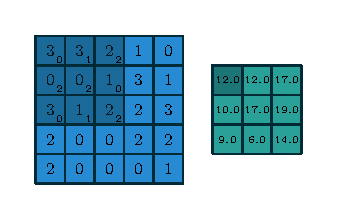
\includegraphics[width=0.32\textwidth]{pdf/numerical_no_padding_no_strides_00.pdf}
    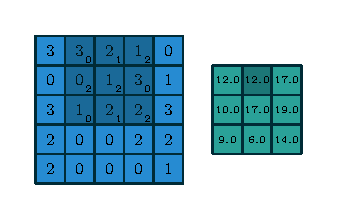
\includegraphics[width=0.32\textwidth]{pdf/numerical_no_padding_no_strides_01.pdf}
    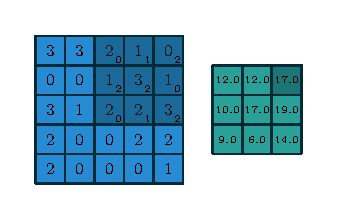
\includegraphics[width=0.32\textwidth]{pdf/numerical_no_padding_no_strides_02.pdf}
    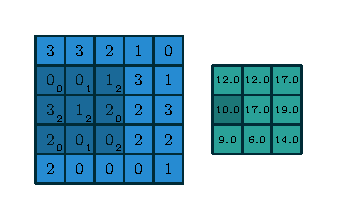
\includegraphics[width=0.32\textwidth]{pdf/numerical_no_padding_no_strides_03.pdf}
    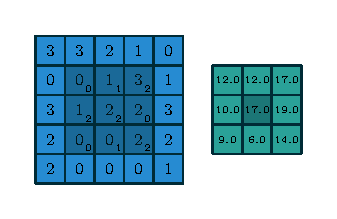
\includegraphics[width=0.32\textwidth]{pdf/numerical_no_padding_no_strides_04.pdf}
    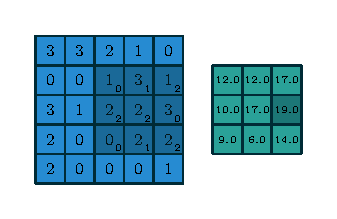
\includegraphics[width=0.32\textwidth]{pdf/numerical_no_padding_no_strides_05.pdf}
    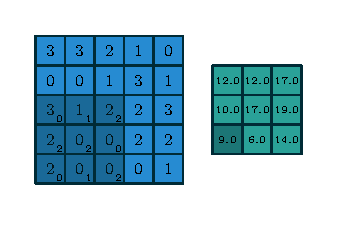
\includegraphics[width=0.32\textwidth]{pdf/numerical_no_padding_no_strides_06.pdf}
    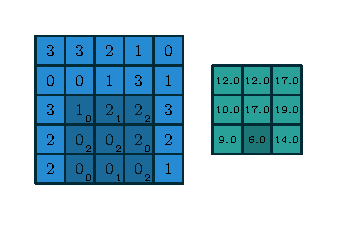
\includegraphics[width=0.32\textwidth]{pdf/numerical_no_padding_no_strides_07.pdf}
    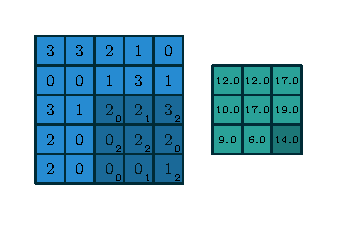
\includegraphics[width=0.32\textwidth]{pdf/numerical_no_padding_no_strides_08.pdf}
    \caption{\label{fig:numerical_no_padding_no_strides} Computing the output
        values of a discrete convolution.}
\end{figure}

\begin{figure}[p]
    \centering
    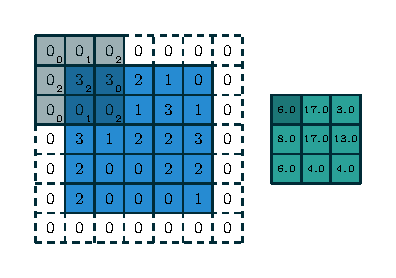
\includegraphics[width=0.32\textwidth]{pdf/numerical_padding_strides_00.pdf}
    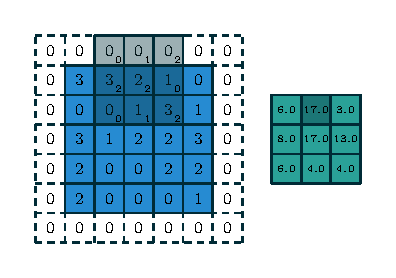
\includegraphics[width=0.32\textwidth]{pdf/numerical_padding_strides_01.pdf}
    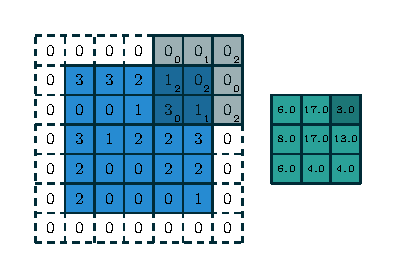
\includegraphics[width=0.32\textwidth]{pdf/numerical_padding_strides_02.pdf}
    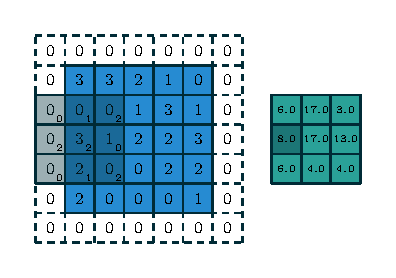
\includegraphics[width=0.32\textwidth]{pdf/numerical_padding_strides_03.pdf}
    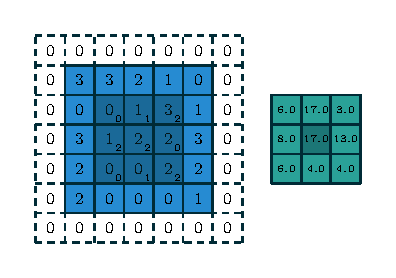
\includegraphics[width=0.32\textwidth]{pdf/numerical_padding_strides_04.pdf}
    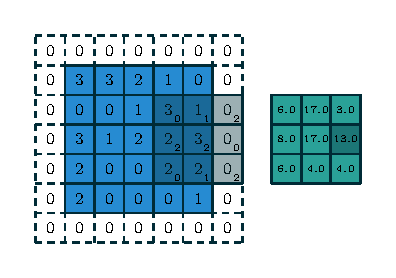
\includegraphics[width=0.32\textwidth]{pdf/numerical_padding_strides_05.pdf}
    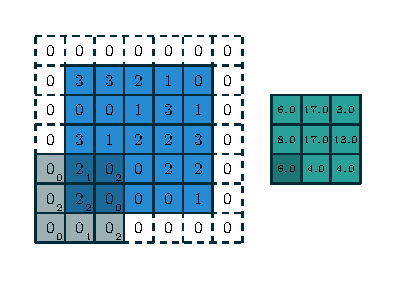
\includegraphics[width=0.32\textwidth]{pdf/numerical_padding_strides_06.pdf}
    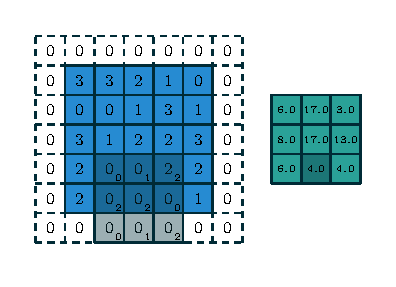
\includegraphics[width=0.32\textwidth]{pdf/numerical_padding_strides_07.pdf}
    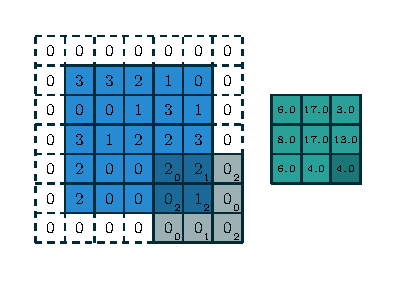
\includegraphics[width=0.32\textwidth]{pdf/numerical_padding_strides_08.pdf}
    \caption{\label{fig:numerical_padding_strides} Computing the output values
        of a discrete convolution for $N = 2$, $i_1 = i_2 = 5$, $k_1 = k_2 = 3$,
        $s_1 = s_2 = 2$, and $p_1 = p_2 = 1$.}
\end{figure}

\noindent slides across the input feature map. At each location, the product
between each element of the kernel and the input element it overlaps is computed
and the results are summed up to obtain the output in the current location. The
procedure can be repeated using different kernels to form as many output feature
maps as desired (\autoref{fig:full_picture}). The final outputs of this procedure
are called {\em output feature maps}.\footnote{%
    While there is a distinction between convolution and cross-correlation from
    a signal processing perspective, the two become interchangeable when the
    kernel is learned. For the sake of simplicity and to stay consistent with
    most of the machine learning literature, the term {\em convolution\/}
    will be used in this guide.}
If there are multiple input feature maps, the kernel will have to be
3-dimensional -- or, equivalently each one of the feature maps will be
convolved with a distinct kernel -- and the resulting feature maps will
be summed up elementwise to produce the output feature map.

The convolution depicted in \autoref{fig:numerical_no_padding_no_strides} is an
instance of a 2-D convolution, but it can be generalized to N-D convolutions.
For instance, in a 3-D convolution, the kernel would be a {\em cuboid\/} and
would slide across the height, width and depth of the input feature map.

The collection of kernels defining a discrete convolution has a shape
corresponding to some permutation of $(n, m, k_1, \ldots, k_N)$, where

\begin{equation*}
\begin{split}
    n &\equiv \text{number of output feature maps},\\
    m &\equiv \text{number of input feature maps},\\
    k_j &\equiv \text{kernel size along axis $j$}.
\end{split}
\end{equation*}

The following properties affect the output size $o_j$ of a convolutional layer
along axis $j$:

\begin{itemize}
    \item $i_j$: input size along axis $j$,
    \item $k_j$: kernel size along axis $j$,
    \item $s_j$: stride (distance between two consecutive positions of the
        kernel) along axis $j$,
    \item $p_j$: zero padding (number of zeros concatenated at the beginning and
        at the end of an axis) along axis $j$.
\end{itemize}

\noindent For instance, \autoref{fig:numerical_padding_strides} shows a $3
\times 3$ kernel applied to a $5 \times 5$ input padded with a $1 \times 1$
border of zeros using $2 \times 2$ strides.

Note that strides constitute a form of \emph{subsampling}. As an alternative to
being interpreted as a measure of how much the kernel is translated, strides
can also be viewed as how much of the output is retained. For instance, moving
the kernel by hops of two is equivalent to moving the kernel by hops of one but
retaining only odd output elements (\autoref{fig:strides_subsampling}).

\begin{figure}[p]
    \centering
    \begin{tikzpicture}[scale=.35,every node/.style={minimum size=1cm}, on grid]
        \begin{scope}[xshift=0cm,yshift=0cm]
            \begin{scope}[xshift=0cm,yshift=0cm]
                \draw[draw=base03,fill=violet,thick]
                    (0,0) grid (5,5) rectangle (0,0);
            \end{scope}
            \begin{scope}[xshift=0.5cm,yshift=0.5cm]
                \draw[draw=base03,fill=blue,thick]
                    (0,0) grid (5,5) rectangle (0,0);
            \end{scope}
        \end{scope}
        \foreach \x in {-10,1,11} {%
            \begin{scope}[xshift=\x cm,yshift=10cm]
                \begin{scope}[xshift=0cm,yshift=0cm]
                    \draw[draw=base03,fill=violet,thick]
                        (0,0) grid (3,3) rectangle (0,0);
                \end{scope}
                \begin{scope}[xshift=0.5cm,yshift=0.5cm]
                    \draw[draw=base03,fill=blue,thick]
                        (0,0) grid (3,3) rectangle (0,0);
                \end{scope}
            \end{scope}
            \begin{scope}[xshift=\x cm,yshift=20cm]\begin{scope}[xshift=0.5cm]
                \draw[draw=base03,fill=cyan,thick]
                    (0,0) grid (3,3) rectangle (0,0);
            \end{scope}\end{scope}
        }
        \begin{scope}[xshift=1cm,yshift=30cm]
            \foreach \s in {0.0,0.5,1.0} {%
                \begin{scope}[xshift=\s cm,yshift=\s cm]
                    \draw[draw=base03,fill=cyan,thick]
                        (0,0) grid (3,3) rectangle (0,0);
                \end{scope}
            }
        \end{scope}
        \draw[->, thick] (-0.5,2.5) to (-8.5,9.5);
        \draw[->, thick] (3,6) to (3,9.5);
        \draw[->, thick] (6,3.5) to (12.5,9.5);
        \draw[thick]  (-8,14.5) to (-8,16);
        \draw[->, thick]  (-8,18) to (-8,19.5);
        \node[thick] (p1) at (-8,17) {$+$};
        \draw[thick]  (3,14.5) to (3,16);
        \draw[->, thick]  (3,18) to (3,19.5);
        \node[thick] (p2) at (3,17) {$+$};
        \draw[thick]  (13,14.5) to (13,16);
        \draw[->, thick]  (13,18) to (13,19.5);
        \node[thick] (p3) at (13,17) {$+$};
        \draw[->, thick]  (-8,23.5) to (2,29.5);
        \draw[->, thick]  (3,23.5) to (2.5,29.5);
        \draw[->, thick]  (13,23.5) to (3,29.5);
    \end{tikzpicture}
    \caption{\label{fig:full_picture} A convolution mapping from two input
        feature maps to three output feature maps using a $3 \times 2 \times 3
        \times 3$ collection of kernels $\mathbf{w}$. In the left pathway, input
        feature map 1 is convolved with kernel $\mathbf{w}_{1,1}$ and input
        feature map 2 is convolved with kernel $\mathbf{w}_{1,2}$, and the
        results are summed together elementwise to form the first output feature
        map. The same is repeated for the middle and right pathways to form the
        second and third feature maps, and all three output feature maps are
        grouped together to form the output.}
\end{figure}

\begin{figure}[p]
    \centering
    \begin{tikzpicture}[scale=.35,every node/.style={minimum size=1cm}, on grid]
        \begin{scope}[xshift=0,yshift=0cm]
            \begin{scope}[xshift=0cm,yshift=0cm]
                \draw[draw=base03,fill=blue,thick] (0,0) grid (5,5) rectangle (0,0);
                \draw[fill=base02, opacity=0.4] (0,2) rectangle (3,5);
            \end{scope}
            \begin{scope}[xshift=7cm,yshift=1.5cm]
                \draw[draw=base03,fill=cyan,thick] (0,0) grid (2,2) rectangle (0,0);
            \end{scope}
        \end{scope}
        \draw[draw=base03, ->, thick] (2.6,3.5) to  (4.5,3.5);
        \draw[draw=base03, ->, thick] (1.5,2.4) to (1.5,0.5);
        \draw[draw=base03, ->, thick] (5.25, 2.5) to (6.75, 2.5);
        \begin{scope}[xshift=12cm,yshift=0cm]
            \begin{scope}[xshift=0cm,yshift=0cm]
                \draw[draw=base03,fill=blue,thick] (0,0) grid (5,5) rectangle (0,0);
                \draw[fill=base02, opacity=0.4] (0,2) rectangle (3,5);
            \end{scope}
            \begin{scope}[xshift=7cm,yshift=1cm]
                \draw[draw=base03,fill=cyan,thick] (0,0) grid (3,3) rectangle (0,0);
                \draw[draw=base03] (1,0) -- (2,1) -- (2,0) -- (1,1);
                \draw[draw=base03] (0,1) -- (1,2) -- (1,1) -- (0,2);
                \draw[draw=base03] (1,1) -- (2,2) -- (2,1) -- (1,2);
                \draw[draw=base03] (2,1) -- (3,2) -- (3,1) -- (2,2);
                \draw[draw=base03] (1,2) -- (2,3) -- (2,2) -- (1,3);
            \end{scope}
            \begin{scope}[xshift=12cm,yshift=1.5cm]
                \draw[draw=base03,fill=cyan,thick] (0,0) grid (2,2) rectangle (0,0);
            \end{scope}
        \end{scope}
        \draw[draw=base03, ->, thick] (14.6,3.5) to  (15.5,3.5);
        \draw[draw=base03, ->, thick] (15.6,3.5) to  (16.5,3.5);
        \draw[draw=base03, ->, thick] (13.5,2.4) to (13.5,1.5);
        \draw[draw=base03, ->, thick] (13.5,1.4) to (13.5,0.5);
        \draw[draw=base03, ->, thick] (17.25, 2.5) to (18.75, 2.5);
        \draw[draw=base03, ->, thick] (22.25, 2.5) to (23.75, 2.5);
    \end{tikzpicture}
    \caption{\label{fig:strides_subsampling} An alternative way of viewing
        strides. Instead of translating the $3 \times 3$ kernel by increments of
        $s = 2$ (left), the kernel is translated by increments of $1$ and only
        one in $s = 2$ output elements is retained (right).}
\end{figure}

\section{Pooling}

In addition to discrete convolutions themselves, {\em pooling\/} operations
make up another important building block in CNNs. Pooling operations reduce
the size of feature maps by using some function to summarize subregions, such
as taking the average or the maximum value.

Pooling works by sliding a window across the input and feeding the content of
the window to a {\em pooling function}. In some sense, pooling works very much
like a discrete convolution, but replaces the linear combination described by
the kernel with some other function. \autoref{fig:numerical_average_pooling}
provides an example for average pooling, and \autoref{fig:numerical_max_pooling}
does the same for max pooling.

The following properties affect the output size $o_j$ of a pooling layer
along axis $j$:

\begin{itemize}
    \item $i_j$: input size along axis $j$,
    \item $k_j$: pooling window size along axis $j$,
    \item $s_j$: stride (distance between two consecutive positions of the
        pooling window) along axis $j$.
\end{itemize}

\begin{figure}[p]
    \centering
    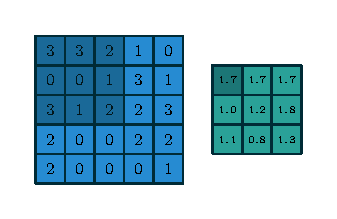
\includegraphics[width=0.32\textwidth]{pdf/numerical_average_pooling_00.pdf}
    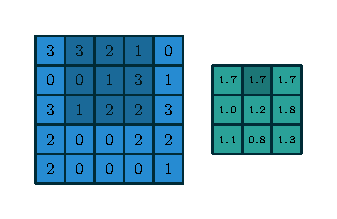
\includegraphics[width=0.32\textwidth]{pdf/numerical_average_pooling_01.pdf}
    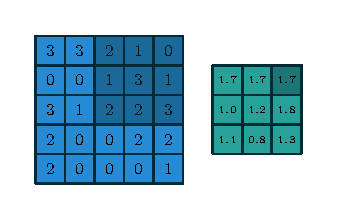
\includegraphics[width=0.32\textwidth]{pdf/numerical_average_pooling_02.pdf}
    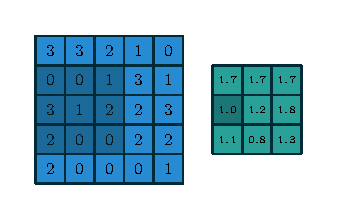
\includegraphics[width=0.32\textwidth]{pdf/numerical_average_pooling_03.pdf}
    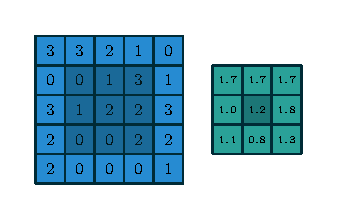
\includegraphics[width=0.32\textwidth]{pdf/numerical_average_pooling_04.pdf}
    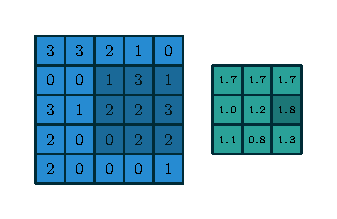
\includegraphics[width=0.32\textwidth]{pdf/numerical_average_pooling_05.pdf}
    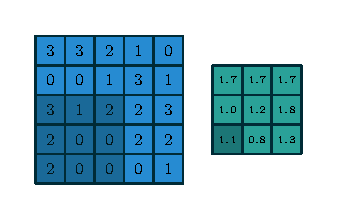
\includegraphics[width=0.32\textwidth]{pdf/numerical_average_pooling_06.pdf}
    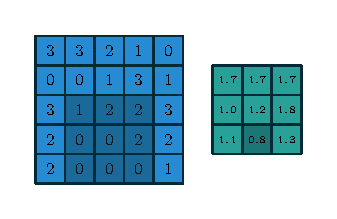
\includegraphics[width=0.32\textwidth]{pdf/numerical_average_pooling_07.pdf}
    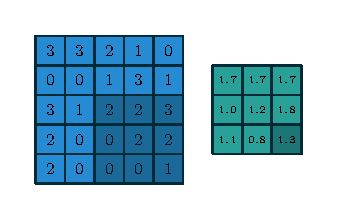
\includegraphics[width=0.32\textwidth]{pdf/numerical_average_pooling_08.pdf}
    \caption{\label{fig:numerical_average_pooling} Computing the output values
        of a $3 \times 3$ average pooling operation on a $5 \times 5$ input
        using $1 \times 1$ strides.}
\end{figure}

\begin{figure}[p]
    \centering
    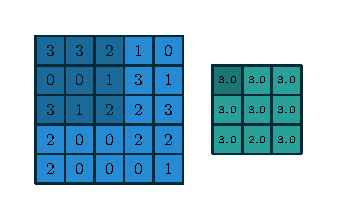
\includegraphics[width=0.32\textwidth]{pdf/numerical_max_pooling_00.pdf}
    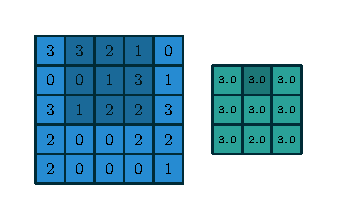
\includegraphics[width=0.32\textwidth]{pdf/numerical_max_pooling_01.pdf}
    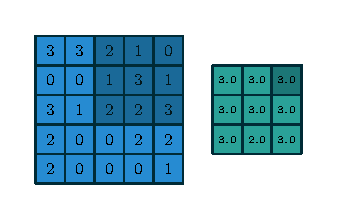
\includegraphics[width=0.32\textwidth]{pdf/numerical_max_pooling_02.pdf}
    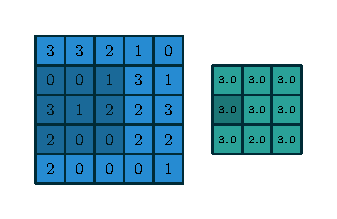
\includegraphics[width=0.32\textwidth]{pdf/numerical_max_pooling_03.pdf}
    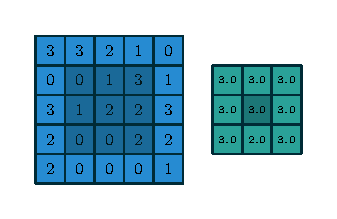
\includegraphics[width=0.32\textwidth]{pdf/numerical_max_pooling_04.pdf}
    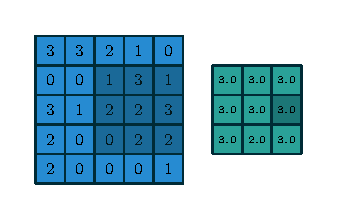
\includegraphics[width=0.32\textwidth]{pdf/numerical_max_pooling_05.pdf}
    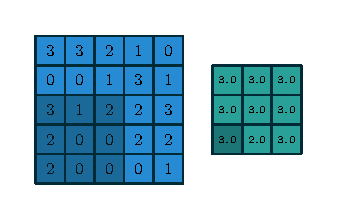
\includegraphics[width=0.32\textwidth]{pdf/numerical_max_pooling_06.pdf}
    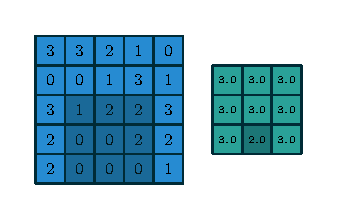
\includegraphics[width=0.32\textwidth]{pdf/numerical_max_pooling_07.pdf}
    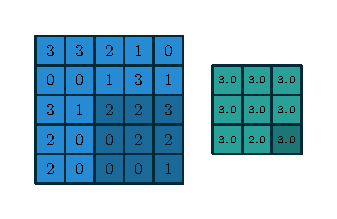
\includegraphics[width=0.32\textwidth]{pdf/numerical_max_pooling_08.pdf}
    \caption{\label{fig:numerical_max_pooling} Computing the output values of a
        $3 \times 3$ max pooling operation on a $5 \times 5$ input using $1
        \times 1$ strides.}
\end{figure}

\chapter{Convolution arithmetic}

The analysis of the relationship between convolutional layer properties is eased
by the fact that they don't interact across axes, i.e., the choice of kernel
size, stride and zero padding along axis $j$ only affects the output size of
axis $j$. Because of that, this chapter will focus on the following simplified
setting:

\begin{itemize}
    \item 2-D discrete convolutions ($N = 2$),
    \item square inputs ($i_1 = i_2 = i$),
    \item square kernel size ($k_1 = k_2 = k$),
    \item same strides along both axes ($s_1 = s_2 = s$),
    \item same zero padding along both axes ($p_1 = p_2 = p$).
\end{itemize}

This facilitates the analysis and the visualization, but keep in mind that the
results outlined here also generalize to the N-D and non-square cases.

\section{No zero padding, unit strides}

The simplest case to analyze is when the kernel just slides across every
position of the input (i.e., $s = 1$ and $p = 0$).
\autoref{fig:no_padding_no_strides} provides an example for $i = 4$ and $k =
3$.

One way of defining the output size in this case is by the number of possible
placements of the kernel on the input. Let's consider the width axis: the kernel
starts on the leftmost part of the input feature map and slides by steps of one
until it touches the right side of the input. The size of the output will be
equal to the number of steps made, plus one, accounting for the initial position
of the kernel (\autoref{fig:no_padding_no_strides_explained}). The same logic
applies for the height axis.

More formally, the following relationship can be inferred:

\begin{relationship}\label{rel:no_padding_no_strides}
For any $i$ and $k$, and for $s = 1$ and $p = 0$,
\begin{equation*}
    o = (i - k) + 1.
\end{equation*}
\end{relationship}

\begin{figure}[p]
    \centering
    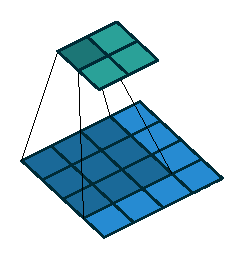
\includegraphics[width=0.24\textwidth]{pdf/no_padding_no_strides_00.pdf}
    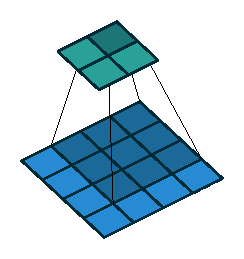
\includegraphics[width=0.24\textwidth]{pdf/no_padding_no_strides_01.pdf}
    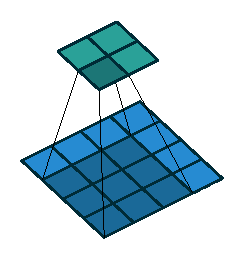
\includegraphics[width=0.24\textwidth]{pdf/no_padding_no_strides_02.pdf}
    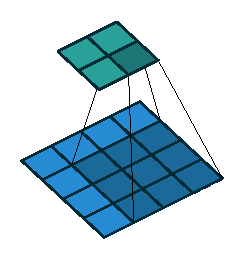
\includegraphics[width=0.24\textwidth]{pdf/no_padding_no_strides_03.pdf}
    \caption{\label{fig:no_padding_no_strides} (No padding, unit strides)
        Convolving a $3 \times 3$ kernel over a $4 \times 4$ input using unit
        strides (i.e., $i = 4$, $k = 3$, $s = 1$ and $p = 0$).}
\end{figure}

\begin{figure}[p]
    \centering
    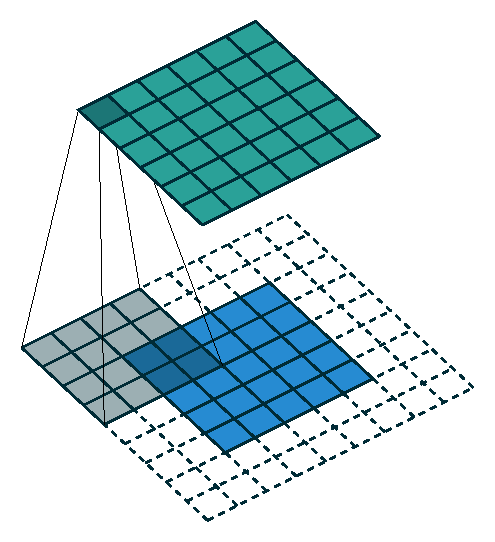
\includegraphics[width=0.24\textwidth]{pdf/arbitrary_padding_no_strides_00.pdf}
    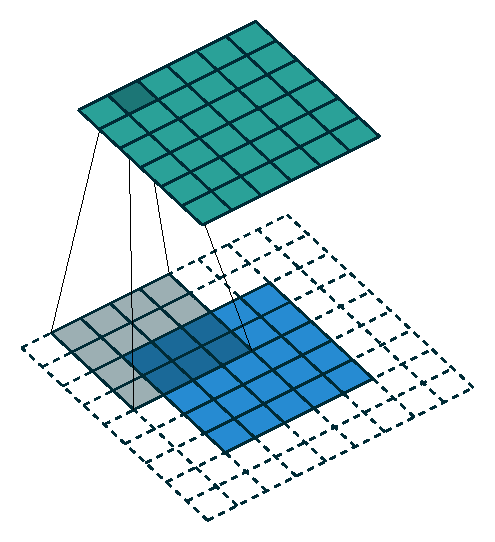
\includegraphics[width=0.24\textwidth]{pdf/arbitrary_padding_no_strides_01.pdf}
    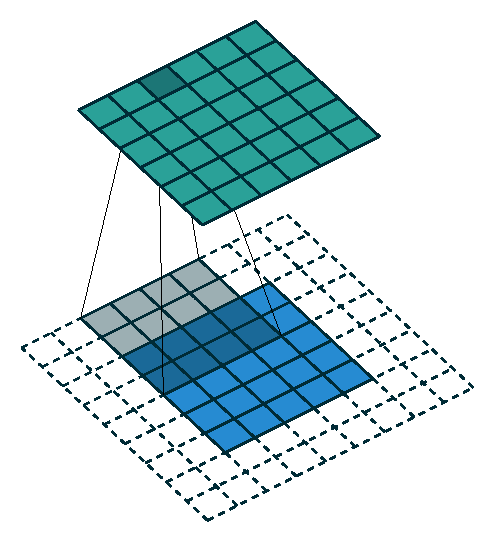
\includegraphics[width=0.24\textwidth]{pdf/arbitrary_padding_no_strides_02.pdf}
    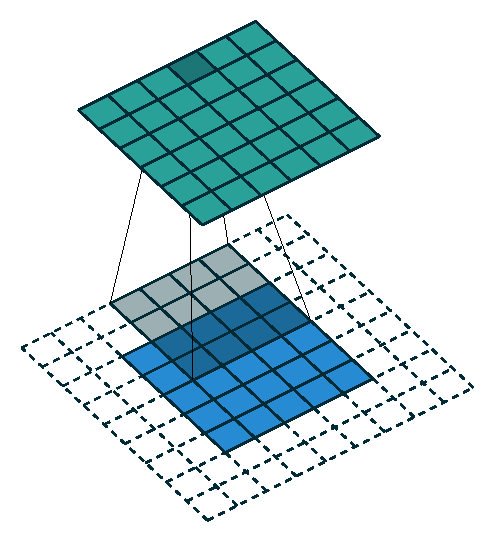
\includegraphics[width=0.24\textwidth]{pdf/arbitrary_padding_no_strides_03.pdf}
    \caption{\label{fig:arbitrary_padding_no_strides} (Arbitrary padding, unit
        strides) Convolving a $4 \times 4$ kernel over a $5 \times 5$ input
        padded with a $2 \times 2$ border of zeros using unit strides (i.e.,
        $i = 5$, $k = 4$, $s = 1$ and $p = 2$).}
\end{figure}

\begin{figure}[p]
    \centering
    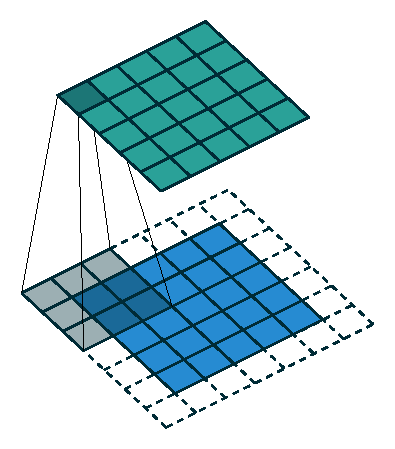
\includegraphics[width=0.24\textwidth]{pdf/same_padding_no_strides_00.pdf}
    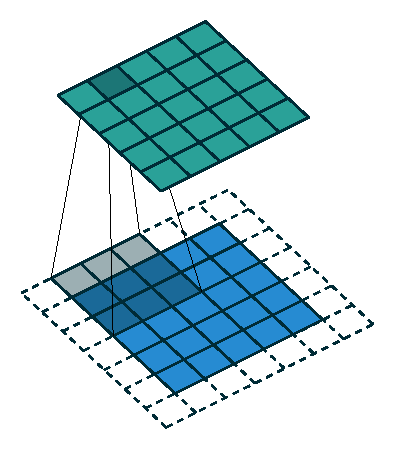
\includegraphics[width=0.24\textwidth]{pdf/same_padding_no_strides_01.pdf}
    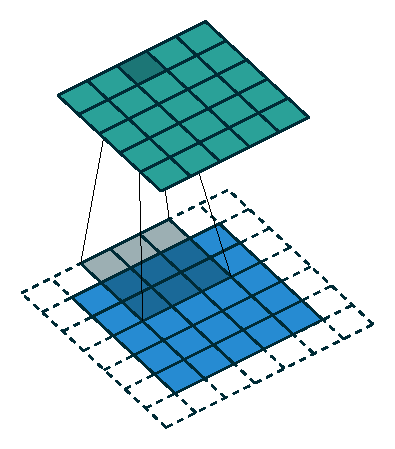
\includegraphics[width=0.24\textwidth]{pdf/same_padding_no_strides_02.pdf}
    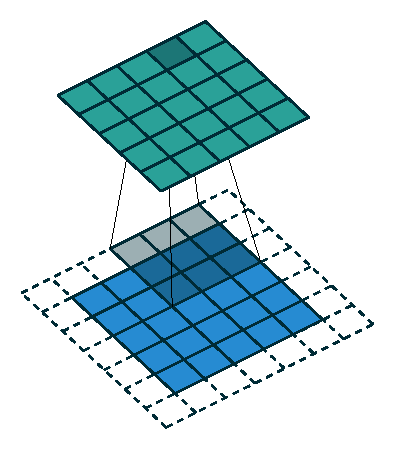
\includegraphics[width=0.24\textwidth]{pdf/same_padding_no_strides_03.pdf}
    \caption{\label{fig:same_padding_no_strides} (Half padding, unit strides)
        Convolving a $3 \times 3$ kernel over a $5 \times 5$ input using half
        padding and unit strides (i.e., $i = 5$, $k = 3$, $s = 1$ and $p = 1$).}
\end{figure}

\begin{figure}[p]
    \centering
    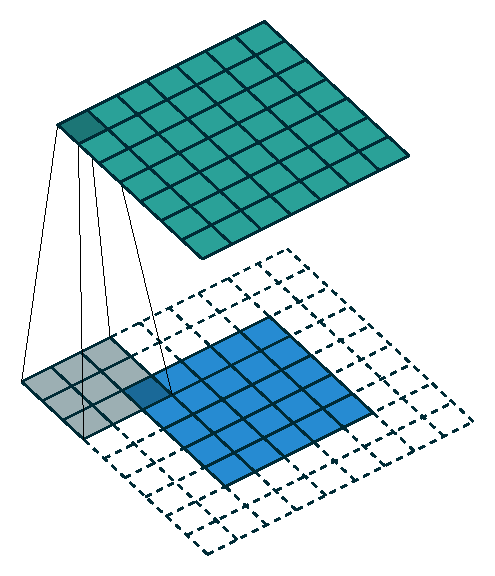
\includegraphics[width=0.24\textwidth]{pdf/full_padding_no_strides_00.pdf}
    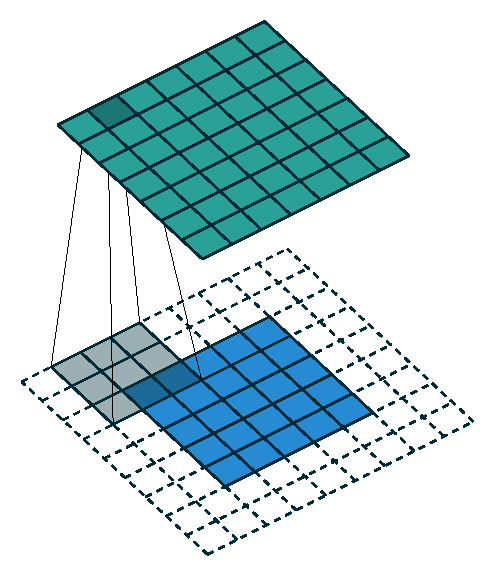
\includegraphics[width=0.24\textwidth]{pdf/full_padding_no_strides_01.pdf}
    \includegraphics[width=0.24\textwidth]{pdf/full_padding_no_strides_02.pdf}
    \includegraphics[width=0.24\textwidth]{pdf/full_padding_no_strides_03.pdf}
    \caption{\label{fig:full_padding_no_strides} (Full padding, unit strides)
        Convolving a $3 \times 3$ kernel over a $5 \times 5$ input using full
        padding and unit strides (i.e., $i = 5$, $k = 3$, $s = 1$ and $p = 2$).}
\end{figure}

\section{Zero padding, unit strides}

To factor in zero padding (i.e., only restricting to $s = 1$), let's consider
its effect on the effective input size: padding with $p$ zeros changes the
effective input size from $i$ to $i + 2p$. In the general case,
\autoref{rel:no_padding_no_strides} can then be used to infer the following
relationship:

\begin{relationship}\label{rel:arbitrary_padding_no_strides}
For any $i$, $k$ and $p$, and for $s = 1$,
\begin{equation*}
    o = (i - k) + 2p + 1.
\end{equation*}
\end{relationship}

\noindent \autoref{fig:arbitrary_padding_no_strides} provides an example for $i
= 5$, $k = 4$ and $p = 2$.

In practice, two specific instances of zero padding are used quite extensively
because of their respective properties. Let's discuss them in more detail.

\subsection{Half (same) padding}

Having the output size be the same as the input size (i.e., $o = i$) can be a
desirable property:

\begin{relationship}\label{rel:same_padding_no_strides}
For any $i$ and for $k$ odd ($k = 2n + 1, \quad n \in \mathbb{N}$), $s = 1$ and
$p = \lfloor k / 2 \rfloor = n$,
\begin{equation*}
\begin{split}
    o &= i + 2 \lfloor k / 2 \rfloor - (k - 1) \\
      &= i + 2n - 2n \\
      &= i.
\end{split}
\end{equation*}
\end{relationship}

\noindent This is sometimes referred to as {\em half\/} (or {\em same\/})
padding. \autoref{fig:same_padding_no_strides} provides an example for
$i = 5$, $k = 3$ and (therefore) $p = 1$.

\subsection{Full padding}

While convolving a kernel generally {\em decreases\/} the output size with
respect to the input size, sometimes the opposite is required. This can be
achieved with proper zero padding:

\begin{relationship}\label{rel:full_padding_no_strides}
For any $i$ and $k$, and for $p = k - 1$ and $s = 1$,
\begin{equation*}
\begin{split}
    o &= i + 2(k - 1) - (k - 1) \\
      &= i + (k - 1).
\end{split}
\end{equation*}
\end{relationship}

\noindent This is sometimes referred to as {\em full\/} padding, because in this
setting every possible partial or complete superimposition of the kernel on the
input feature map is taken into account. \autoref{fig:full_padding_no_strides}
provides an example for $i = 5$, $k = 3$ and (therefore) $p = 2$.

\section{No zero padding, non-unit strides}

All relationships derived so far only apply for unit-strided convolutions.
Incorporating non unitary strides requires another inference leap. To
facilitate the analysis, let's momentarily ignore zero padding (i.e., $s > 1$
and $p = 0$). \autoref{fig:no_padding_strides} provides an example for $i =
5$, $k = 3$ and $s = 2$.

Once again, the output size can be defined in terms of the number of possible
placements of the kernel on the input. Let's consider the width axis: the
kernel starts as usual on the leftmost part of the input, but this time it
slides by steps of size $s$ until it touches the right side of the input. The
size of the output is again equal to the number of steps made, plus one,
accounting for the initial position of the kernel
(\autoref{fig:no_padding_strides_explained}). The same logic applies for the
height axis.

From this, the following relationship can be inferred:

\begin{relationship}\label{rel:no_padding_strides}
For any $i$, $k$ and $s$, and for $p = 0$,
\begin{equation*}
    o = \left\lfloor \frac{i - k}{s} \right\rfloor + 1.
\end{equation*}
\end{relationship}

\noindent The floor function accounts for the fact that sometimes the last
possible step does {\em not\/} coincide with the kernel reaching the end of the
input, i.e., some input units are left out (see
\autoref{fig:padding_strides_odd} for an example of such a case).

\section{Zero padding, non-unit strides}

The most general case (convolving over a zero padded input using non-unit
strides) can be derived by applying \autoref{rel:no_padding_strides} on an
effective input of size $i + 2p$, in analogy to what was done for
\autoref{rel:arbitrary_padding_no_strides}:

\begin{relationship}\label{rel:padding_strides}
For any $i$, $k$, $p$ and $s$,
\begin{equation*}
    o = \left\lfloor \frac{i + 2p - k}{s} \right\rfloor + 1.
\end{equation*}
\end{relationship}

\noindent As before, the floor function means that in some cases a convolution
will produce the same output size for multiple input sizes. More specifically,
if $i + 2p - k$ is a multiple of $s$, then any input size $j = i + a, \quad a
\in \{0,\ldots,s - 1\}$ will produce the same output size. Note that this
ambiguity applies only for $s > 1$.

\autoref{fig:padding_strides} shows an example with $i = 5$, $k = 3$, $s = 2$
and $p = 1$, while \autoref{fig:padding_strides_odd} provides an example for
$i = 6$, $k = 3$, $s = 2$ and $p = 1$. Interestingly, despite having different
input sizes these convolutions share the same output size. While this doesn't
affect the analysis for {\em convolutions}, this will complicate the analysis
in the case of {\em transposed convolutions}.

\begin{figure}[p]
    \centering
    \includegraphics[width=0.24\textwidth]{pdf/no_padding_strides_00.pdf}
    \includegraphics[width=0.24\textwidth]{pdf/no_padding_strides_01.pdf}
    \includegraphics[width=0.24\textwidth]{pdf/no_padding_strides_02.pdf}
    \includegraphics[width=0.24\textwidth]{pdf/no_padding_strides_03.pdf}
    \caption{\label{fig:no_padding_strides} (No zero padding, arbitrary
        strides) Convolving a $3 \times 3$ kernel over a $5 \times 5$ input
        using $2 \times 2$ strides (i.e., $i = 5$, $k = 3$, $s = 2$ and
        $p = 0$).}
\end{figure}

\begin{figure}[p]
    \centering
    \includegraphics[width=0.24\textwidth]{pdf/padding_strides_00.pdf}
    \includegraphics[width=0.24\textwidth]{pdf/padding_strides_01.pdf}
    \includegraphics[width=0.24\textwidth]{pdf/padding_strides_02.pdf}
    \includegraphics[width=0.24\textwidth]{pdf/padding_strides_03.pdf}
    \caption{\label{fig:padding_strides} (Arbitrary padding and strides)
        Convolving a $3 \times 3$ kernel over a $5 \times 5$ input padded with
        a $1 \times 1$ border of zeros using $2 \times 2$ strides (i.e.,
        $i = 5$, $k = 3$, $s = 2$ and $p = 1$).}
\end{figure}

\begin{figure}[p]
    \centering
    \includegraphics[width=0.24\textwidth]{pdf/padding_strides_odd_00.pdf}
    \includegraphics[width=0.24\textwidth]{pdf/padding_strides_odd_01.pdf}
    \includegraphics[width=0.24\textwidth]{pdf/padding_strides_odd_02.pdf}
    \includegraphics[width=0.24\textwidth]{pdf/padding_strides_odd_03.pdf}
    \caption{\label{fig:padding_strides_odd} (Arbitrary padding and strides)
        Convolving a $3 \times 3$ kernel over a $6 \times 6$ input padded with
        a $1 \times 1$ border of zeros using $2 \times 2$ strides (i.e.,
        $i = 6$, $k = 3$, $s = 2$ and $p = 1$). In this case, the bottom row
        and right column of the zero padded input are not covered by the
        kernel.}
\end{figure}

\begin{figure}[p]
    \centering
    \begin{subfigure}[t]{0.48\textwidth}
        \centering
        \begin{tikzpicture}[scale=.35,every node/.style={minimum size=1cm},
                            on grid]
            \draw[fill=blue] (0,0) rectangle (5,5);
            \draw[draw=base03, thick] (0,0) grid (5,5);
            \draw[fill=base02, opacity=0.4] (0,2) rectangle (3,5);
            \draw[step=10mm, base03, thick] (0,2) grid (3,5);
            \draw[draw=base03, ->, thick] (2.6,3.5) to  (3.5,3.5);
            \draw[draw=base03, ->, thick] (3.6,3.5) to  (4.5,3.5);
            \draw[draw=base03, ->, thick] (1.5,2.4) to  (1.5,1.5);
            \draw[draw=base03, ->, thick] (1.5,1.4) to  (1.5,0.5);
        \end{tikzpicture}
        \caption{\label{fig:no_padding_no_strides_explained} The kernel has to
            slide two steps to the right to touch the right side of the input
            (and equivalently downwards).  Adding one to account for the
            initial kernel position, the output size is $3 \times 3$.}
    \end{subfigure}
    ~
    \begin{subfigure}[t]{0.48\textwidth}
        \centering
        \begin{tikzpicture}[scale=.35,every node/.style={minimum size=1cm},
                            on grid]
            \draw[fill=blue] (0,0) rectangle (5,5);
            \draw[draw=base03, thick] (0,0) grid (5,5);
            \draw[fill=base02, opacity=0.4] (0,2) rectangle (3,5);
            \draw[step=10mm, base03, thick] (0,2) grid (3,5);
            \draw[draw=base03, ->, thick] (2.5,3.5) to  (4.5,3.5);
            \draw[draw=base03, ->, thick] (1.5,2.5) to  (1.5,0.5);
        \end{tikzpicture}
        \caption{\label{fig:no_padding_strides_explained} The kernel has to
            slide one step of size two to the right to touch the right side of
            the input (and equivalently downwards).  Adding one to account for
            the initial kernel position, the output size is $2 \times 2$.}
    \end{subfigure}
    \caption{Counting kernel positions.}
\end{figure}

\chapter{Pooling arithmetic}

In a neural network, pooling layers provide invariance to small translations of
the input. The most common kind of pooling is \emph{max pooling}, which
consists in splitting the input in (usually non-overlapping) patches and
outputting the maximum value of each patch. Other kinds of pooling exist, e.g.,
mean or average pooling, which all share the same idea of aggregating the input
locally by applying a non-linearity to the content of some patches \citep{%
boureau-cvpr-10,boureau-icml-10,boureau-iccv-11,ICML2011Saxe_551}.

Some readers may have noticed that the treatment of convolution arithmetic only
relies on the assumption that some function is repeatedly applied onto subsets
of the input. This means that the relationships derived in the previous chapter
can be reused in the case of pooling arithmetic. Since pooling does not involve
zero padding, the relationship describing the general case is as follows:

\begin{relationship}\label{rel:pooling}
For any $i$, $k$ and $s$,
\begin{equation*}
    o = \left\lfloor \frac{i - k}{s} \right\rfloor + 1.
\end{equation*}
\end{relationship}

\noindent This relationship holds for any type of pooling.

\chapter{Transposed convolution arithmetic}

The need for transposed convolutions generally arises from the desire to use a
transformation going in the opposite direction of a normal convolution, i.e.,
from something that has the shape of the output of some convolution to
something that has the shape of its input while maintaining a connectivity
pattern that is compatible with said convolution. For instance, one might use
such a transformation as the decoding layer of a convolutional autoencoder or to
project feature maps to a higher-dimensional space.

Once again, the convolutional case is considerably more complex than the
fully-connected case, which only requires to use a weight matrix whose shape
has been transposed. However, since every convolution boils down to an
efficient implementation of a matrix operation, the insights gained from the
fully-connected case are useful in solving the convolutional case.

Like for convolution arithmetic, the dissertation about transposed convolution
arithmetic is simplified by the fact that transposed convolution properties
don't interact across axes.

The chapter will focus on the following setting:

\begin{itemize}
    \item 2-D transposed convolutions ($N = 2$),
    \item square inputs ($i_1 = i_2 = i$),
    \item square kernel size ($k_1 = k_2 = k$),
    \item same strides along both axes ($s_1 = s_2 = s$),
    \item same zero padding along both axes ($p_1 = p_2 = p$).
\end{itemize}

\noindent Once again, the results outlined generalize to the N-D and non-square
cases.

\section{Convolution as a matrix operation}

Take for example the convolution represented in
\autoref{fig:no_padding_no_strides}. If the input and output were to be unrolled
into vectors from left to right, top to bottom, the convolution could be
represented as a sparse matrix $\mathbf{C}$ where the non-zero elements are the
elements $w_{i,j}$ of the kernel (with $i$ and $j$ being the row and column of
the kernel respectively):
\begin{equation*}
\setcounter{MaxMatrixCols}{20}
\resizebox{.98\hsize}{!}{$%
    \begin{pmatrix}%
    w_{0,0} & w_{0,1} & w_{0,2} & 0       & w_{1,0} & w_{1,1} & w_{1,2} & 0       &
    w_{2,0} & w_{2,1} & w_{2,2} & 0       & 0       & 0       & 0       & 0       \\
    0       & w_{0,0} & w_{0,1} & w_{0,2} & 0       & w_{1,0} & w_{1,1} & w_{1,2} &
    0       & w_{2,0} & w_{2,1} & w_{2,2} & 0       & 0       & 0       & 0       \\
    0       & 0       & 0       & 0       & w_{0,0} & w_{0,1} & w_{0,2} & 0       &
    w_{1,0} & w_{1,1} & w_{1,2} & 0       & w_{2,0} & w_{2,1} & w_{2,2} & 0       \\
    0       & 0       & 0       & 0       & 0       & w_{0,0} & w_{0,1} & w_{0,2} &
    0       & w_{1,0} & w_{1,1} & w_{1,2} & 0       & w_{2,0} & w_{2,1} & w_{2,2} \\
    \end{pmatrix}$}
\end{equation*}

This linear operation takes the input matrix flattened as a 16-dimensional
vector and produces a 4-dimensional vector that is later reshaped as the $2
\times 2$ output matrix.

Using this representation, the backward pass is easily obtained by transposing
$\mathbf{C}$; in other words, the error is backpropagated by multiplying the
loss with $\mathbf{C}^T$. This operation takes a 4-dimensional vector as input
and produces a 16-dimensional vector as output, and its connectivity pattern is
compatible with $\mathbf{C}$ by construction.

Notably, the kernel $\mathbf{w}$ defines both the matrices $\mathbf{C}$ and
$\mathbf{C}^T$ used for the forward and backward passes.

\section{Transposed convolution}

Let's now consider what would be required to go the other way around, i.e., map
from a 4-dimensional space to a 16-dimensional space, while keeping the
connectivity pattern of the convolution depicted in
\autoref{fig:no_padding_no_strides}. This operation is known as a {\em
transposed convolution}.

Transposed convolutions -- also called {\em fractionally strided convolutions\/}
-- work by swapping the forward and backward passes of a convolution. One way to
put it is to note that the kernel defines a convolution, but whether it's a
direct convolution or a transposed convolution is determined by how the forward
and backward passes are computed.

For instance, although the kernel $\mathbf{w}$ defines a convolution whose
forward and backward passes are computed by multiplying with $\mathbf{C}$ and
$\mathbf{C}^T$ respectively, it {\em also\/} defines a transposed convolution
whose forward and backward passes are computed by multiplying with
$\mathbf{C}^T$ and $(\mathbf{C}^T)^T = \mathbf{C}$ respectively.\footnote{The
    transposed convolution operation can be thought of as the gradient of {\em
    some\/} convolution with respect to its input, which is usually how
    transposed convolutions are implemented in practice.}

Finally note that it is always possible to emulate a transposed convolution with
a direct convolution. The disadvantage is that it usually involves adding many
columns and rows of zeros to the input, resulting in a much less efficient
implementation.

Building on what has been introduced so far, this chapter will proceed somewhat
backwards with respect to the convolution arithmetic chapter, deriving the
properties of each transposed convolution by referring to the direct
convolution with which it shares the kernel, and defining the equivalent direct
convolution.

\section{No zero padding, unit strides, transposed}

The simplest way to think about a transposed convolution is by computing the
output shape of the direct convolution for a given input shape first, and then
inverting the input and output shapes for the transposed convolution.

Let's consider the convolution of a $3 \times 3$ kernel on a $4 \times 4$
input with unitary stride and no padding (i.e., $i = 4$, $k = 3$, $s = 1$ and
$p = 0$). As depicted in \autoref{fig:no_padding_no_strides}, this produces a
$2 \times 2$ output. The transpose of this convolution will then have an output
of shape $4 \times 4$ when applied on a $2 \times 2$ input.

Another way to obtain the result of a transposed convolution is to apply an
equivalent -- but much less efficient -- direct convolution. The example
described so far could be tackled by convolving a $3 \times 3$ kernel over a
$2 \times 2$ input padded with a $2 \times 2$ border of zeros using unit
strides (i.e., $i' = 2$, $k' = k$, $s' = 1$ and $p' = 2$), as shown in
\autoref{fig:no_padding_no_strides_transposed}. Notably, the kernel's and
stride's sizes remain the same, but the input of the transposed convolution is
now zero padded.\footnote{Note that although
    equivalent to applying the transposed matrix, this visualization adds a lot
    of zero multiplications in the form of zero padding.  This is done here for
    illustration purposes, but it is inefficient, and software implementations
    will normally not perform the useless zero multiplications.}

One way to understand the logic behind zero padding is to consider the
connectivity pattern of the transposed convolution and use it to guide the
design of the equivalent convolution. For example, the top left pixel of the
input of the direct convolution only contribute to the top left pixel of the
output, the top right pixel is only connected to the top right output pixel,
and so on.

To maintain the same connectivity pattern in the equivalent convolution it is
necessary to zero pad the input in such a way that the first (top-left)
application of the kernel only touches the top-left pixel, i.e., the padding
has to be equal to the size of the kernel minus one.

Proceeding in the same fashion it is possible to determine similar observations
for the other elements of the image, giving rise to the following relationship:

\begin{relationship}\label{rel:no_padding_no_strides_transposed}
A convolution described by $s = 1$, $p = 0$ and $k$ has an associated
transposed convolution described by $k' = k$, $s' = s$ and $p' = k - 1$ and its
output size is
\begin{equation*}
    o' = i' + (k - 1).
\end{equation*}
\end{relationship}

Interestingly, this corresponds to a fully padded convolution with unit
strides.

\section{Zero padding, unit strides, transposed}

Knowing that the transpose of a non-padded convolution is equivalent to
convolving a zero padded input, it would be reasonable to suppose that the
transpose of a zero padded convolution is equivalent to convolving an input
padded with {\em less\/} zeros.

It is indeed the case, as shown in
\autoref{fig:arbitrary_padding_no_strides_transposed} for $i = 5$, $k = 4$ and
$p = 2$.

Formally, the following relationship applies for zero padded convolutions:

\begin{relationship}\label{rel:arbitrary_padding_no_strides_transposed}
A convolution described by $s = 1$, $k$ and $p$ has an
associated transposed convolution described by $k' = k$, $s' = s$ and $p' = k -
p - 1$ and its output size is
\begin{equation*}
    o' = i' + (k - 1) - 2p.
\end{equation*}
\end{relationship}

\begin{figure}[p]
    \centering
    \includegraphics[width=0.24\textwidth]{pdf/no_padding_no_strides_transposed_00.pdf}
    \includegraphics[width=0.24\textwidth]{pdf/no_padding_no_strides_transposed_01.pdf}
    \includegraphics[width=0.24\textwidth]{pdf/no_padding_no_strides_transposed_02.pdf}
    \includegraphics[width=0.24\textwidth]{pdf/no_padding_no_strides_transposed_03.pdf}
    \caption{\label{fig:no_padding_no_strides_transposed} The transpose of
        convolving a $3 \times 3$ kernel over a $4 \times 4$ input using unit
        strides (i.e., $i = 4$, $k = 3$, $s = 1$ and $p = 0$). It is equivalent
        to convolving a $3 \times 3$ kernel over a $2 \times 2$ input padded
        with a $2 \times 2$ border of zeros using unit strides (i.e., $i' = 2$,
        $k' = k$, $s' = 1$ and $p' = 2$).}
\end{figure}

\begin{figure}[p]
    \centering
    \includegraphics[width=0.24\textwidth]{pdf/arbitrary_padding_no_strides_transposed_00.pdf}
    \includegraphics[width=0.24\textwidth]{pdf/arbitrary_padding_no_strides_transposed_01.pdf}
    \includegraphics[width=0.24\textwidth]{pdf/arbitrary_padding_no_strides_transposed_02.pdf}
    \includegraphics[width=0.24\textwidth]{pdf/arbitrary_padding_no_strides_transposed_03.pdf}
    \caption{\label{fig:arbitrary_padding_no_strides_transposed} The transpose
        of convolving a $4 \times 4$ kernel over a $5 \times 5$ input padded
        with a $2 \times 2$ border of zeros using unit strides (i.e., $i = 5$,
        $k = 4$, $s = 1$ and $p = 2$). It is equivalent to convolving a $4
        \times 4$ kernel over a $6 \times 6$ input padded with a $1 \times 1$
        border of zeros using unit strides (i.e., $i' = 6$, $k' = k$, $s' = 1$
        and $p' = 1$).}
\end{figure}

\begin{figure}[p]
    \centering
    \includegraphics[width=0.24\textwidth]{pdf/same_padding_no_strides_transposed_00.pdf}
    \includegraphics[width=0.24\textwidth]{pdf/same_padding_no_strides_transposed_01.pdf}
    \includegraphics[width=0.24\textwidth]{pdf/same_padding_no_strides_transposed_02.pdf}
    \includegraphics[width=0.24\textwidth]{pdf/same_padding_no_strides_transposed_03.pdf}
    \caption{\label{fig:same_padding_no_strides_transposed} The transpose of
        convolving a $3 \times 3$ kernel over a $5 \times 5$ input using half
        padding and unit strides (i.e., $i = 5$, $k = 3$, $s = 1$ and $p = 1$).
        It is equivalent to convolving a $3 \times 3$ kernel over a $5 \times 5$
        input using half padding and unit strides (i.e., $i' = 5$, $k' = k$, $s'
        = 1$ and $p' = 1$).}
\end{figure}

\subsection{Half (same) padding, transposed}

By applying the same inductive reasoning as before, it is reasonable to expect
that the equivalent convolution of the transpose of a half padded convolution
is itself a half padded convolution, given that the output size of a half
padded convolution is the same as its input size. Thus the following relation
applies:

\begin{relationship}\label{rel:half_padding_no_strides_transposed}
A convolution described by $k = 2n + 1, \quad n \in \mathbb{N}$, $s = 1$ and $p
= \lfloor k / 2 \rfloor = n$ has an associated transposed convolution described
by $k' = k$, $s' = s$ and $p' = p$ and its output size is
\begin{equation*}
\begin{split}
    o' &= i' + (k - 1) - 2p \\
       &= i' + 2n - 2n \\
       &= i'.
\end{split}
\end{equation*}
\end{relationship}

\autoref{fig:same_padding_no_strides_transposed} provides an example for $i =
5$, $k = 3$ and (therefore) $p = 1$.

\subsection{Full padding, transposed}

Knowing that the equivalent convolution of the transpose of a non-padded
convolution involves full padding, it is unsurprising that the equivalent of
the transpose of a fully padded convolution is a non-padded convolution:

\begin{relationship}\label{rel:full_padding_no_strides_transposed}
A convolution described by $s = 1$, $k$ and $p = k - 1$ has an
associated transposed convolution described by $k' = k$, $s' = s$ and $p' = 0$
and its output size is
\begin{equation*}
\begin{split}
    o' &= i' + (k - 1) - 2p \\
       &= i' - (k - 1)
\end{split}
\end{equation*}
\end{relationship}

\autoref{fig:full_padding_no_strides_transposed} provides an example for $i =
5$, $k = 3$ and (therefore) $p = 2$.

\section{No zero padding, non-unit strides, transposed}

Using the same kind of inductive logic as for zero padded convolutions, one
might expect that the transpose of a convolution with $s > 1$ involves an
equivalent convolution with $s < 1$. As will be explained, this is a valid
intuition, which is why transposed convolutions are sometimes called {\em
fractionally strided convolutions}.

\autoref{fig:no_padding_strides_transposed} provides an example for $i = 5$, $k
= 3$ and $s = 2$ which helps understand what fractional strides involve: zeros
are inserted {\em between\/} input units, which makes the kernel move around at
a slower pace than with unit strides.\footnote{Doing so is inefficient and
    real-world implementations avoid useless multiplications by zero, but
    conceptually it is how the transpose of a strided convolution can be
    thought of.}

For the moment, it will be assumed that the convolution is non-padded ($p = 0$)
and that its input size $i$ is such that $i - k$ is a multiple of $s$. In that
case, the following relationship holds:

\begin{relationship}\label{rel:no_padding_strides_transposed}
A convolution described by $p = 0$, $k$ and $s$ and whose input
size is such that $i - k$ is a multiple of $s$, has an associated transposed
convolution described by $\tilde{i}'$, $k' = k$, $s' = 1$ and $p' = k - 1$,
where $\tilde{i}'$ is the size of the stretched input obtained by adding
$s - 1$ zeros between each input unit, and its output size is
\begin{equation*}
\begin{split}
    o' = s (i' - 1) + k.
\end{split}
\end{equation*}
\end{relationship}

\begin{figure}[p]
    \centering
    \includegraphics[width=0.24\textwidth]{pdf/full_padding_no_strides_transposed_00.pdf}
    \includegraphics[width=0.24\textwidth]{pdf/full_padding_no_strides_transposed_01.pdf}
    \includegraphics[width=0.24\textwidth]{pdf/full_padding_no_strides_transposed_02.pdf}
    \includegraphics[width=0.24\textwidth]{pdf/full_padding_no_strides_transposed_03.pdf}
    \caption{\label{fig:full_padding_no_strides_transposed} The transpose of
        convolving a $3 \times 3$ kernel over a $5 \times 5$ input using full
        padding and unit strides (i.e., $i = 5$, $k = 3$, $s = 1$ and $p = 2$).
        It is equivalent to convolving a $3 \times 3$ kernel over a $7 \times 7$
        input using unit strides (i.e., $i' = 7$, $k' = k$, $s' = 1$ and $p' =
        0$).}
\end{figure}

\begin{figure}[p]
    \centering
    \includegraphics[width=0.24\textwidth]{pdf/no_padding_strides_transposed_00.pdf}
    \includegraphics[width=0.24\textwidth]{pdf/no_padding_strides_transposed_01.pdf}
    \includegraphics[width=0.24\textwidth]{pdf/no_padding_strides_transposed_02.pdf}
    \includegraphics[width=0.24\textwidth]{pdf/no_padding_strides_transposed_03.pdf}
    \caption{\label{fig:no_padding_strides_transposed} The transpose of
        convolving a $3 \times 3$ kernel over a $5 \times 5$ input using $2
        \times 2$ strides (i.e., $i = 5$, $k = 3$, $s = 2$ and $p = 0$). It is
        equivalent to convolving a $3 \times 3$ kernel over a $2 \times 2$ input
        (with $1$ zero inserted between inputs) padded with a $2 \times 2$
        border of zeros using unit strides (i.e., $i' = 2$, $\tilde{i}' = 3$, $k'
        = k$, $s' = 1$ and $p' = 2$).}
\end{figure}

\begin{figure}[p]
    \centering
    \includegraphics[width=0.24\textwidth]{pdf/padding_strides_transposed_00.pdf}
    \includegraphics[width=0.24\textwidth]{pdf/padding_strides_transposed_01.pdf}
    \includegraphics[width=0.24\textwidth]{pdf/padding_strides_transposed_02.pdf}
    \includegraphics[width=0.24\textwidth]{pdf/padding_strides_transposed_03.pdf}
    \caption{\label{fig:padding_strides_transposed} The transpose of convolving
        a $3 \times 3$ kernel over a $5 \times 5$ input padded with a $1 \times
        1$ border of zeros using $2 \times 2$ strides (i.e., $i = 5$, $k = 3$, $s
        = 2$ and $p = 1$). It is equivalent to convolving a $3 \times 3$ kernel
        over a $2 \times 2$ input (with $1$ zero inserted between inputs) padded
        with a $1 \times 1$ border of zeros using unit strides (i.e., $i' = 3$,
        $\tilde{i}' = 5$, $k' = k$, $s' = 1$ and $p' = 1$).}
\end{figure}

\section{Zero padding, non-unit strides, transposed}

When the convolution's input size $i$ is such that $i + 2p - k$ is a multiple
of $s$, the analysis can extended to the zero padded case by combining
\autoref{rel:arbitrary_padding_no_strides_transposed} and
\autoref{rel:no_padding_strides_transposed}:

\begin{relationship}\label{rel:padding_strides_transposed}
A convolution described by $k$, $s$ and $p$ and whose
input size $i$ is such that $i + 2p - k$ is a multiple of $s$ has an associated
transposed convolution described by $\tilde{i}'$, $k' = k$, $s' = 1$ and
$p' = k - p - 1$, where $\tilde{i}'$ is the size of the stretched input
obtained by adding $s - 1$ zeros between each input unit, and its output size
is
\begin{equation*}
\begin{split}
    o' = s (i' - 1) + k - 2p.
\end{split}
\end{equation*}
\end{relationship}

\autoref{fig:padding_strides_transposed} provides an example for $i = 5$, $k =
3$, $s = 2$ and $p = 1$.

The constraint on the size of the input $i$ can be relaxed by introducing
another parameter $a \in \{0, \ldots, s - 1\}$ that allows to distinguish
between the $s$ different cases that all lead to the same $i'$:

\begin{relationship}\label{rel:padding_strides_transposed_odd}
A convolution described by $k$, $s$ and $p$ has an
associated transposed convolution described by $a$, $\tilde{i}'$, $k' = k$, $s'
= 1$ and $p' = k - p - 1$, where $\tilde{i}'$ is the size of the stretched
input obtained by adding $s - 1$ zeros between each input unit, and $a = (i +
2p - k) \mod s$ represents the number of zeros added to the top and right edges
of the input, and its output size is
\begin{equation*}
\begin{split}
    o' = s (i' - 1) + a + k - 2p.
\end{split}
\end{equation*}
\end{relationship}

\autoref{fig:padding_strides_odd_transposed} provides an example for $i = 6$, $k
= 3$, $s = 2$ and $p = 1$.

\begin{figure}[p]
    \centering
    \includegraphics[width=0.24\textwidth]{pdf/padding_strides_odd_transposed_00.pdf}
    \includegraphics[width=0.24\textwidth]{pdf/padding_strides_odd_transposed_01.pdf}
    \includegraphics[width=0.24\textwidth]{pdf/padding_strides_odd_transposed_02.pdf}
    \includegraphics[width=0.24\textwidth]{pdf/padding_strides_odd_transposed_03.pdf}
    \caption{\label{fig:padding_strides_odd_transposed} The transpose of
        convolving a $3 \times 3$ kernel over a $6 \times 6$ input padded with a
        $1 \times 1$ border of zeros using $2 \times 2$ strides (i.e., $i = 6$,
        $k = 3$, $s = 2$ and $p = 1$). It is equivalent to convolving a $3
        \times 3$ kernel over a $2 \times 2$ input (with $1$ zero inserted
        between inputs) padded with a $1 \times 1$ border of zeros (with an
        additional border of size $1$ added to the top and right edges) using
        unit strides (i.e., $i' = 3$, $\tilde{i}' = 5$, $a = 1$, $k' = k$, $s' =
        1$ and $p' = 1$).}
\end{figure}

%================================== SECTION ==================================
\section{Recurrent networks}\label{sec:i}
Write something about RNNs, LSTMs, GRUs
 % uncomment if you want part I
\chapter{Object classification with Recurrent Neural Networks}\label{sec:renet}

\emph{Classification} is a broad task that consists in predicting to which
category an input belongs to, out of some $k$ given categories. The system is
usually required to compute a function $f: \RR \to {0, \dots, k-1}$ that
assigns each input to a class. This can be thought as a discrimination task,
where the algorithm is expected to learn similarities and differences between
categories in order to characterize each class.

Some examples of classification are spam detection (classify a message as being
spam or not), credit card fraud detection (identify if a transaction is legit
or not), optical character recognition (OCR) (convert hand-written text to an
electronic document, by classifying each character), speech understanding
(given an utterance from a user, detect the sentence that was pronounced),
medical diagnosis (given the symptoms predict the illness and suggest a cure),
stock trading (determine if a stock should be bought, help or sold, from
current and historical data), shape detection (classify a hand-drawn drawing
from, e.g., a touch screen, as a specific shape) and emotion recognition (given
a text, classify it as being positive, neutral or negative)

\emph{Object recognition} is an instance of this task that takes an image as an
input and is expected to return the id of the main class represented in the
image. This is usually achieved by computing the probability distribution over
the classes -- i.e. the confidence of the algorithm for each class to be the
main class in the scene -- and then picking the one with highest score.

One downside of this method is that small and big mistakes are penalized the
same, i.e., the prediction is considered wrong whether the right class is the
second most probable class in the distribution or is considered extremely
unlikely by the algorithm. For this reason, some competitions such as
e.g.,~ImageNet~\citep{imagenet_cvpr09, ILSVRCarxiv14}, propose multiple
challenges where the top-3 or top-5 guesses are considered, i.e., where an
image is considered correctly predicted if the correct class is in the top
$3$ or $5$ guesses of the network.

Traditionally the computer vision community used to address this task with
heavily hand-engineered systems that typically resorted to finding easily
detectable elements in the image -- such as e.g. edges or corners -- and
computing a descriptor of the surrounding patch. Many detectors~\cite{
dufournaud2000matching,harris1988combined,mikolajczyk2001indexing,
lowe2004distinctive,mikolajczyk2005performance} and descriptors~\cite{
lowe1999object,mikolajczyk2005performance,belongie2002shape} have been proposed
to this end, until in 2012 a deep convolutional neural network shifted the
balance toward learned ANNs indefinitely~\citep{Krizhevsky-2012}. Since then
CNN-based models dominated the object recognition scene.

This chapter presents ReNet, one of the main contributions of this thesis.
The ReNet model is a deep neural network architecture for object recognition,
based on recurrent neural networks. The main idea behind this project is to
propose an alternative to the typical CNN-based approach to object
classification problems. The ReNet model replaces in fact the ubiquitous
convolution+pooling layers of deep CNNs with four recurrent neural networks
that sweep horizontally and vertically in both directions across the image.

The following sections motivate the model in the context of the state of the
art at the time it was conceived, describe the ReNet model in detail and
present the results of its evaluation on three widely-used object recognition
benchmarks, namely  MNIST~\citep{Lecun99objectrecognition},
CIFAR-10~\citep{KrizhevskyHinton2009} and SVHN~\citep{Netzer-wkshp-2011}. The
experiments reveal that the ReNet model performs comparably to convolutional
neural networks on all these datasets, suggesting the potential of RNNs as a
competitive alternative to the conventional deep convolutional neural networks
for image related tasks.


\section{Rationale}
Convolutional neural networks~\cite[CNN,][]{Fukushima80,LeCun89} have become the
method of choice for object recognition after the impressive improvement on the
state of the art of~\cite{Krizhevsky-2012}. CNNs have proved to be successful
at a variety of benchmark problems including, but not limited to, handwritten
digit recognition~\citep[see, e.g.,][]{Ciresan-2012}, natural image
classification~\citep[see, e.g.,][]{Lin2014,Simonyan2015,szegedy2014going},
house number recognition~\citep[see, e.g.,][]{Goodfellow+et+al-ICLR2014a},
traffic sign recognition~\citep[see, e.g.,][]{Ciresan-et-al-2012}, as well as
for speech recognition~\citep[see, e.g.,][]{Hamid2012, sainath2013,
toth2014combining}.  Furthermore, image representations from CNNs trained to
recognize objects on a large set of more than one million
images~\citep{Simonyan2015,szegedy2014going} have been found to be extremely
helpful in performing other computer vision tasks such as image caption
generation~\citep[see, e.g.,][]{Vinyals-et-al-arxiv2014,Xu-et-al-arxiv2015},
video description generation~\citep[see, e.g.,][]{Li2015} and object
localization/detection~\citep[see, e.g.,][]{Sermanet14}.

While the CNN has been especially successful in computer vision, recurrent
neural networks (RNN) have become the method of choice for modeling sequential
data, such as text and sound. Natural language processing (NLP) applications
include language modeling~\citep[see, e.g.,][]{Mikolov-thesis-2012}, and
machine translation~\citep{Sutskever-et-al-NIPS2014,Cho2014,
bahdanau2014neural}. Other popular areas of application include offline
handwriting recognition/generation~\citep{Graves+Schmidhuber-2009,
Graves-et-al-NIPS2007,Graves-arxiv2013} and speech recognition~\citep{
Chorowski-et-al-arxiv2014,Graves+Jaitly-ICML2014}. RNNs have also been used
together with CNNs in speech recognition~\citep{sainath2015}. The recent
revival of RNNs has largely been due to advances in learning
algorithms~\citep{Pascanu+al-ICML2013-small,Martens+Sutskever-ICML2011} and
model architectures~\citep{Pascanu-et-al-ICLR2014,Hochreiter+Schmidhuber-1997,
Cho2014}.

The architecture of ReNet is related and inspired by this earlier work, but
relies on purely uni-dimensional RNNs coupled in a novel way, rather than on a
multi-dimensional RNN. The basic idea behind the ReNet model is to replace each
convolutional layer (with convolution+pooling making up a layer) in the CNN
with four RNNs that sweep over lower-layer features in different directions:
(1) bottom to top, (2) top to bottom, (3) left to right and (4) right to left.
The recurrent layer ensures that each feature activation in its output is an
activation at the specific location \emph{with respect to the whole image}, in
contrast to the usual convolution+pooling layer which only has a local context
window. The lowest layer of the model sweeps over the input image, with
subsequent layers operating on extracted representations from the layer below,
forming a hierarchical representation of the input.

\citet{Graves+Schmidhuber-2009} have demonstrated an RNN-based object
recognition system for offline Arabic handwriting recognition. The main
difference between ReNet and the model of \citet{Graves+Schmidhuber-2009} is
that it uses the usual sequence RNN, instead of the multidimensional RNN. The
way ReNet has been conceived allows in fact to capture the context of the
image without being forced to resort to multidimensional RNNs: the latter two
RNNs (or, equivalently, the last bidirectional RNN), work on the hidden states
computed by the first two RNNs (or the first bidirectional RNN). This allows
to use plain RNNs instead of the more complex multidimensional ones, while
making each output activation of the layer be computed with respect to the
whole input image.

One important consequence of the proposed approach compared to the
multidimensional RNN is that the number of RNNs at each layer scales linearly
with respect to the number of dimensions $d$ of the input image ($2d$). A
multidimensional RNN, on the other hand, requires an exponential number of RNNs
at each layer ($2^d$). Furthermore, the proposed variant is more easily
parallelizable, as each RNN is dependent only along a horizontal or vertical
sequence of patches. This architectural distinction results in the ReNet model
being much more amenable to distributed computing than that
of~\citet{Graves+Schmidhuber-2009}.

\vfill

\section{Model Description}\label{sec:renet_model}

\begin{figure}
    \centering
    \includegraphics[width=0.3\textwidth]{pdf/renet_first_layer.pdf}
    \caption{A one-layer ReNet}
    \label{fig:networklayer}
    \vspace{-3mm}
\end{figure}

Let us denote by $X=\left\{x_{i,j}\right\}$ the input image or the feature map
from the layer below, where $X \in \RR^{w \times h \times c}$ with $w$, $h$ and
$c$ the width, height and number of channels, or the feature dimensionality,
respectively. Given a receptive field (or patch) size of $w_p \times h_p$, we
split the input image $X$ into a set of $I \times J$ (non-overlapping) patches
$P = \left\{ p_{i,j} \right\}$, where $I = \frac{w}{w_p}$, $J = \frac{h}{h_p}$
and $p_{i,j} \in \RR^{w_p \times h_p \times c}$ is the $(i,j)$-th patch of the
input image. The first index $i$ is the horizontal index and the other index
$j$ is the vertical index.

First, the image is swept vertically with two RNNs, with one RNN working in
a bottom-up direction and the other working in a top-down direction.
Each RNN takes as an input one (flattened) patch at a time and updates its
hidden state, working \emph{along each column} $j$ of the split input image $X$.
\begin{align}
    v^F_{i,j} = f_{\text{VFWD}}(z^F_{i,j-1},p_{i,j}), &\text{ for
    }j=1,\cdots, J\\
    v^R_{i,j} = f_{\text{VREV}}(z^R_{i,j+1},p_{i,j}), &\text{ for
    }j=J,\cdots,1
\end{align}

Note that $f_{\text{VFWD}}$ and $f_{\text{VREV}}$ return the activation of the
recurrent hidden state, and may be implemented either as a simple $\tanh$ layer,
as a gated recurrent layer~\citep{Cho2014} or as a long short-term memory
layer~\citep{Hochreiter+Schmidhuber-1997}.

After this vertical, bidirectional sweep, the intermediate hidden states
$v^F_{i,j}$ and $v^R_{i,j}$ are concatenated at each location $(i,j)$ to get a
composite feature map $V= \left\{ v_{i,j} \right\}_{i=1,\ldots,I}^{
j=1,\ldots,J}$, where $v_{i,j} \in \RR^{2d}$ and $d$ is the number of recurrent
units.  Each $v_{i,j}$ is now the activation of a feature detector at the
location $(i,j)$ with respect to all the patches in the $j$-th column of the
original input ($p_{i, j}$ for all $i$).

Next, the obtained composite feature map $V$ is swept horizontally with two
different RNNs ($f_{\text{HFWD}}$ and $f_{\text{HREV}}$). In a similar manner
as for the vertical sweep, these RNNs work along each row of $V$ and produce an
output feature map $H = \left\{ h_{i,j} \right\}$, where $h_{i,j} \in
\RR^{2d}$. In this representation, each vector $h_{i,j}$ represents the
features of the original image patch $p_{i,j}$ \emph{in the context of the
whole image}.

This is a critical feature of this model, in fact just one layer (to be
precise, two sub-layers) allows to capture the full context of the image,
irrespective of the image size. This is possible thanks to the (potential)
ability of RNNs to store in their memory any information that is relevant to
retain the context of the part of the image that has been processed. The first
two RNNs capture the horizontal dependencies in both directions. By reading
their composite feature map, the second pair of RNNs has access in each
position to a "summary" of the corresponding row. This is processed vertically,
to capture the missing dependencies between rows. This intra- and inter-row
processing results in a final composite feature map where each position is
specific to a pixel (or patch) of the image but has information on the full
image. Conversely, to span over the whole image with CNN-based architectures
would require many more layers, whose number depend on the size of the input
image.

Even if each ReNet layer captures the full input context, it is clearly still
possible to stack multiple ReNet layers on top of each other into a deep
network. Let us denote by $\phi$ the function from the input image (or feature
map) $X$ of one ReNet layer to the output feature map $H$
(see~\autoref{fig:networklayer} for a graphical illustration). It is possible
to compute a composition of functions $\Phi = \phi_1(\phi_2(\phi_3(\dots)))$ by
stacking multiple ReNet layers, to capture increasingly complex features of the
input image.  After any number of recurrent layers are applied to an input
image, the activation at the last recurrent layer may be flattened and fed into
a differentiable classifier to solve an object recognition task. The
experiments on this model, presented in~\autoref{sec:renet_experiments}, used
several fully-connected layers followed by a softmax classifier, as shown
in~\autoref{fig:network}.

The deep ReNet is a smooth, continuous function, and the parameters (those from
the RNNs as well as from the fully-connected layers) can be estimated by the
stochastic gradient descent algorithm with the gradient computed by
backpropagation algorithm~\citep[see, e.g.,][]{BP86} to maximize the
log-likelihood.

\subsection{Differences between LeNet and ReNet}
\label{sec:lenetrenet}

\begin{figure}[h]
    \centering
    \includegraphics[width=0.9\textwidth]{img/lenet5.jpg}
    \caption{The LeNet network}
    \label{fig:lenet}
    \vspace{-3mm}
\end{figure}

This section will use LeNet (see~\autoref{fig:lenet}) to refer to the canonical
convolutional neural network as shown by \citet{LeCun89}. There are many
similarities and differences between the ReNet model and a convolutional neural
network. The main key points of comparison will be highlighted in what follows.

At each layer, both networks apply the same set of filters to patches of the
input image or of the feature map from the layer below. ReNet, however,
propagates information through lateral connections that span across the whole
image, while LeNet exploits local information only. The lateral connections
should help extract a more compact feature representation of the input image at
each layer, which can be accomplished by the lateral connections
removing/resolving redundant features at different locations of the image. This
should allow ReNet resolve small displacements of features across multiple
consecutive patches. Also, the lack of this type of lateral connection in LeNet
may lead to many more levels of convolution+pooling layers in order to detect
redundant features from different parts of the image.

LeNet max-pools the activations of each filter over a small region to achieve
local translation invariance. In contrast, the proposed ReNet does not use any
pooling due to the existence of learned lateral connections. The lateral
connection in ReNet can emulate the local competition among features induced by
the max-pooling in LeNet.  This does not mean that it is not possible to use
max-pooling in ReNet. The use of max-pooling in the ReNet could be helpful in
reducing the dimensionality of the feature map, resulting in lower computational
cost.

Max-pooling as used in LeNet may prove problematic when building a
convolutional autoencoder whose decoder is an inverse\footnote{
    All the forward arrows from the input to the output in the original LeNet
    are reversed.
}
of LeNet, as the max operator is not invertible. The proposed
ReNet is end-to-end smooth and differentiable, making it more suited to be used
as a decoder in the autoencoder or any of its probabilistic variants~\citep[see,
e.g.,][]{Kingma+Welling-ICLR2014}.

In some sense, each layer of the ReNet can be considered as a variant of a usual
convolution+pooling layer, where pooling is replaced with lateral connections,
and convolution is done without any overlap. Similarly, \citet{Springenberg2014}
recently proposed a variant of a usual LeNet which does not use any pooling.
They used convolution with a larger stride to compensate for the lack of
dimensionality reduction by pooling at each layer. However, this approach still
differs from the proposed ReNet in the sense that each feature activation at a
layer is only with respect to a subset of the input image rather than the whole
input image.

The main disadvantage of ReNet is that it is not easily parallelizable, due to
the sequential nature of the recurrent neural network (RNN). LeNet, on the other
hand, is highly parallelizable due to the independence of computing activations
at each layer. The introduction of sequential, lateral connections, however, may
result in more efficient parametrization, requiring a smaller number of
parameters with overall fewer computations, although this needs to be further
explored. Note that this limitation on parallelization applies only to model
parallelism, and any technique for data parallelism may be used for both the
proposed ReNet and the LeNet.

\section{Experiments}\label{sec:renet_experiments}

\subsection{Datasets}

The ReNet model has been evaluated on three widely-used benchmark datasets;
MNIST, CIFAR-10 and the Street View Housing Numbers (SVHN). This section
describes each dataset in detail.

\paragraph{MNIST}

\begin{figure}[h]
    \centering
    \includegraphics[width=0.5\textwidth]{img/mnist_digits.png}
    \caption{Some digits from the MNIST dataset}
    \label{fig:mnist_digits}
\end{figure}

The MNIST dataset~\citep{Lecun99objectrecognition} consists of 70,000
handwritten digits from 0 to 9, centered on a $28\times 28$ square
canvas~(see~\autoref{fig:mnist_digits} for some samples). Each pixel represents
the grayscale in the range of $\left[0, 255\right]$.\footnote{Each pixel has
been scaled to $[0, 1]$ by dividing it with $255$.} It is customary to split
this dataset into 50,000 training samples, 10,000 validation samples and 10,000
test samples. For a fair comparison, the results reported
in~\autoref{sec:renet_results} were obtained following the standard split.

\paragraph{CIFAR-10}

\begin{figure}[h]
    \centering
    \includegraphics[width=0.5\textwidth]{img/cifar-10.png}
    \caption{Some samples of the 10 classes of the CIFAR-10 dataset}
    \label{fig:cifar}
\end{figure}

The CIFAR-10 dataset~\citep{KrizhevskyHinton2009} is a curated subset of the 80
million tiny images dataset~(see~\autoref{fig:cifar} for some samples),
originally released by \citet{Torralba+Fergus+Freeman-2008}. CIFAR-10 contains
60,000 images each of which belongs to one of ten categories: airplane,
automobile, bird, cat, deer, dog, frog, horse, ship and truck. Each image is 32
pixels wide and 32 pixels high with 3 color channels (red, green and blue.)
Following the standard procedure, in the reported experiments the dataset
was split into 40,000 training, 10,000 validation and 10,000 test samples.
Furthermore, zero-phase component analysis (ZCA) was applied and the each pixel
was normalized to have zero-mean and unit-variance across the training samples,
as suggested by \citet{KrizhevskyHinton2009}.

\paragraph{Street View House Numbers}

\begin{figure}[h]
    \centering
    \includegraphics[width=0.5\textwidth]{img/SVHN.png}
    \caption{Some samples of housing numbers from the SVHN dataset}
    \label{fig:svhn}
\end{figure}

The Street View House Numbers (SVHN) dataset~\citep{Netzer-wkshp-2011} consists
of cropped images representing house numbers captured by Google StreetView
vehicles as a part of the Google Maps mapping process. These images consist of
digits 0 through 9 with values in the range of [0, 255] in each of 3
red-green-blue color channels~(see~\autoref{fig:svhn} for some samples). Each
image is 32 pixels wide and 32 pixels high giving a sample dimensionality (32,
32, 3). The number of samples used for the training, validation, and test sets
is 543,949, 60,439, and 26,032 respectively. Each pixel was normalized to have
zero-mean and unit-variance across the training samples.

\subsection{Data Augmentation}

It has been long known that augmenting training data often leads to better
generalization~\citep[see, e.g.,][]{Krizhevsky-2012}. The results reported
in~\autoref{sec:renet_results} were all obtained employing two primary data
augmentations: {\it flipping} and {\it shifting}.

For the flipping data augmentation, the model was presented with samples that
were either flipped horizontally with 25\% chance, or vertically with 25\%
chance, or left unchanged. This technique allows the model to observe ``mirror
images'' of the original images of the dataset during training, increasing the
amount of training data. On SVHN and MNIST only horizontal flipping was used
to prevent the case were an image labelled $6$ is flipped in both direction,
becoming a $9$.

In the case of shifting two policies were adopted. The images were either
shifted by 2 pixels to the left (25\% chance), 2 pixels to the right (25\%
chance) or left as they were. After this first processing, the images were
further shifted either by 2 pixels to the top (25\% chance), 2 pixels to the
bottom (25\% chance) or left as they were. This two-step procedure makes the
model more robust to slight shifting of an object in the image. The shifting
was done without pre-padding the borders of the image, but rather preserving
the original size by dropping the pixels which are shifted out of the input
and shifting in zeros on the opposite side.

The choice of whether to apply these augmentation procedures on each dataset
was chosen on a per-case basis in order to maximize validation performance.

\begin{figure}[t]
    \centering
    \includegraphics[height=.14\textheight,width=\columnwidth]{pdf/renet_svhn.pdf}
    \caption{The ReNet network used for SVHN classification}
    \label{fig:network}
\end{figure}

\subsection{Model Architectures}

The principal parameters that define the architecture of the ReNet model are
the number of ReNet layers ($N_{\text{RE}}$), their corresponding receptive
field sizes ($w_p \times h_p$) and feature dimensionality ($d_{\text{RE}}$),
the number of fully-connected layers ($N_{\text{FC}}$) and their corresponding
numbers ($d_{\text{FC}}$) and types ($f_{\text{FC}}$) of hidden units.

Table~\ref{tbl:architectures} summarizes the settings of these hyperparameters
that performed best on the validation set of the studied datasets.
\autoref{fig:network} is a graphical illustration of the model selected with
this metric for the SVHN dataset.

\begin{table}[t]
    \centering
    \begin{tabular}{l || c | c | c }
        & MNIST & CIFAR-10 & SVHN \\
        \hline
        \hline
    $N_{\text{RE}}$ & 2 & 3 & 3 \\
        \hline
        $w_p \times h_p$ & $[2\times 2]$--$[2 \times 2]$ & $[2\times 2]$--$[2 \times 2]$--$[2
        \times 2]$ & $[2\times 2]$--$[2 \times 2]$--$[2 \times 2]$ \\
        \hline
    $d_{\text{RE}}$ & 256--256 & 320--320--320 & 256--256--256 \\
        \hline
    $N_{\text{FC}}$ & 2 & 1 & 2 \\
        \hline
    $d_{\text{FC}}$ & 4096--4096 & 4096 & 4096--4096 \\
        \hline
    $f_{\text{FC}}$ & $\max(0, x)$ & $\max(0,x)$ & $\max(0,x)$ \\
        \hline
    Flipping & no & yes & no \\
        \hline
    Shifting & yes & yes & yes \\
    \end{tabular}
    \caption{Model architectures used in the experiments. Each row shows
             respectively the number of ReNet layers, the size of the patches,
             the number of neurons of each ReNet layer, the number of fully
             connected layers, the number of neurons of the fully connected
             layers, their activation function and the data augmentation
             procedure employed.}
    \label{tbl:architectures}
\end{table}

\subsubsection{Training}

All the networks have been trained using a recently proposed adaptive learning
rate algorithm, called Adam~\citep{Kingma2014}. In order to reduce overfitting
dropout~\citep{Srivastava14} was applied after each layer, including both the
ReNet layers (after the horizontal and vertical sweeps) and the fully-connected
layers. The input layer was also corrupted by masking out each pixel with
probability $0.2$. Finally, each optimization run was early stopped based
on validation error.

Note that the results reported in~\autoref{sec:renet_results} were obtained
without retraining on the joint training and validation sets. This is a common
technique exploited by many works in the literature to boost the performance
of the best model, selected after a full training on the training set early
stopping on the validation performance. There is no reason not to think that
this would further improve the reported results, but this work was mainly
conceived as a proof of concept rather than to stress on the absolute
performance. This, as well as e.g., ensembling multiple models, can be seen as
one of the many potential areas of exploration for further work in case maximum
performance is sought.

\begin{table}[ht]
    \centering

    \begin{minipage}{0.45\textwidth}
        \centering

        \begin{tabular}{l |  l}
            Test Error & Model  \\
            \hline
0.28\% & \citep{DBLP:conf/icml/WanZZLF13}$\star$ \\
0.31\% & \citep{DBLP:journals/corr/Graham14}$\star$ \\
0.35\% & \citep{DBLP:journals/corr/abs-1003-0358} \\
0.39\% & \citep{DBLP:conf/nips/MairalKHS14}$\star$ \\
0.39\% & \citep{DBLP:journals/corr/LeeXGZT14}$\star$ \\
0.4\% & \citep{DBLP:conf/icdar/SimardSP03}$\star$ \\
0.44\% & \citep{DBLP:journals/corr/Graham14a}$\star$ \\
0.45\% & \citep{Goodfellow2013}$\star$ \\
\bf{0.45\%} & \bf{ReNet} \\
0.47\% & \citep{Lin2014}$\star$ \\
0.52\% & \citep{DBLP:journals/pami/AzzopardiA13} \\
        \end{tabular}

        \vspace{2mm}
        (a) MNIST
    \end{minipage}
    \hfill
    \begin{minipage}{0.45\textwidth}
        \centering

        \begin{tabular}{l |  l}
            Test Error & Model  \\
            \hline
4.5\% & \citep{DBLP:journals/corr/Graham14a}$\star$ \\
6.28\% & \citep{DBLP:journals/corr/Graham14}$\star$ \\
8.8\% & \citep{Lin2014}$\star$ \\
9.35\% & \citep{Goodfellow2013}$\star$ \\
9.39\% & \citep{DBLP:journals/corr/SpringenbergR13}$\star$ \\
9.5\% & \citep{DBLP:conf/nips/SnoekLA12}$\star$ \\
11\% & \citep{Krizhevsky-2012}$\star$ \\
11.10\% & \citep{DBLP:conf/icml/WanZZLF13}$\star$ \\
\bf{12.35\%} & \bf{ReNet} \\
15.13\% & \citep{DBLP:journals/corr/abs-1301-3557}$\star$ \\
15.6\% & \citep{DBLP:journals/corr/abs-1207-0580}$\star$ \\
        \end{tabular}

        \vspace{2mm}
        (b) CIFAR-10
    \end{minipage}

    \vspace{4mm}
    \begin{minipage}{0.45\textwidth}
        \centering
        \begin{tabular}{l |  l}
            Test Error & Model  \\
            \hline
1.92\% & \citep{DBLP:journals/corr/LeeXGZT14}$\star$ \\
2.23\% & \citep{DBLP:conf/icml/WanZZLF13}$\star$ \\
2.35\% & \citep{Lin2014}$\star$ \\
\bf{2.38\%} & \bf{ReNet} \\
2.47\% & \citep{Goodfellow2013}$\star$ \\
2.8\% & \citep{DBLP:journals/corr/abs-1301-3557}$\star$ \\
        \end{tabular}

        \vspace{2mm}
        (c) SVHN
    \end{minipage}
    \hfill
    \begin{minipage}{0.51\textwidth}
        \caption{Generalization errors obtained by the proposed ReNet along
            with those reported by previous works on each of the three
            datasets. For a fair comparison, only results obtained by a single
            model are listed, i.e., no ensembling of multiple models. In the
            case of SVHN, only models trained on the Format 2 (cropped digits)
            dataset are reported. $\star$ denotes a convolutional neural
            network.}
        \label{tbl:result}
    \end{minipage}
\end{table}

\subsection{Results}\label{sec:renet_results}
Table~\ref{tbl:result}, presents the results of ReNet on three datasets, along
with previously reported results.

It is clear that ReNet performs comparably to deep convolutional neural
networks which are the {\it de facto} standard for object recognition. This
suggests that ReNet is a viable alternative to convolutional neural networks
(CNN), even on tasks where CNNs have historically dominated. However, it is
important to notice that ReNet does not outperform state-of-the-art
convolutional neural networks on any of the three benchmark datasets, which
calls for more research in the future.

\section{Conclusions/Discussion}

\paragraph{Choice of Recurrent Units}
Note that the proposed architecture is independent of the chosen recurrent
units. The preliminary experiments on this model showed that gated recurrent
units, either the GRU or the LSTM, outperform a usual sigmoidal unit (affine
transformation followed by an element-wise sigmoid function.) This indirectly
confirms that the model utilizes long-term dependencies across an input image,
and the gated recurrent units help capture these dependencies.

\paragraph{Analysis of the Trained ReNet}
In this paper, we evaluated the proposed ReNet only quantitatively. However, the
accuracies on the test sets do not reveal what kind of image structures the
ReNet has captured in order to perform object recognition. Due to the large
differences between ReNet and LeNet discussed in
Sec.~\ref{sec:lenetrenet}, we expect that the internal behavior of ReNet
will differ from that of LeNet significantly. Further investigation along
the line of \citep{ZeilerFergus14} will be needed, as well exploring ensembles
which combine RNNs and CNNs for bagged prediction.

\paragraph{Computationally Efficient Implementation}
As discussed in Sec.~\ref{sec:lenetrenet}, the proposed ReNet is less
parallelizable due to the sequential nature of the recurrent neural network
(RNN). Although this sequential nature cannot be addressed directly, our
construction of ReNet allows the forward and backward RNNs to be run
independently from each other, which allows for parallel computation.
Furthermore, we can use many parallelization tricks widely used for training
convolutional neural networks such as parallelizing fully-connected layers
~\citep{krizhevsky2014one}, having separate sets of kernels/features in
different processors~\citep{Krizhevsky-2012} and exploiting data parallelism.


% \begin{table}[h]
% \begin{tabular}{ll}
% 0.35\% & Deep Big Simple Neural Nets Excel on Handwritten Digit Recognition \citep{DBLP:journals/corr/abs-1003-0358} \\
% 0.39\% & Convolutional Kernel Networks \citep{DBLP:conf/nips/MairalKHS14} \\
% 0.39\% & Deeply-Supervised Nets \citep{DBLP:journals/corr/LeeXGZT14} \\
% 0.4\% & Best Practices for Convolutional Neural Networks Applied to Visual Document Analysis \citep{DBLP:conf/icdar/SimardSP03} \\
% 0.45\% & Maxout Networks \citep{Goodfellow2013} \\
% \bf{0.45\%} & \bf{ReNet} \\
% 0.47\% & Network in Network \citep{Lin2014} \\
% 0.52\% & Trainable COSFIRE filters for keypoint detection and pattern recognition \citep{DBLP:journals/pami/AzzopardiA13} \\
% \end{tabular}
% \end{table}
%
% MNIST (talk about why we don't compare to dropconnect/multicolumn?)
%
% CIFAR-10 (briefly mention ZCA, flipping, pixel shift)
% \begin{table}[h]
% \begin{tabular}{ll}
% 8.8\% & Network In Network \citep{Lin2014} \\
% 9.32\% & Regularization of Neural Networks using DropConnect \citep{DBLP:conf/icml/WanZZLF13} \\
% 9.35\% & Maxout Networks \citep{Goodfellow2013} \\
% 9.39\% & Improving Deep Neural Networks with Probabilistic Maxout Units \citep{DBLP:journals/corr/SpringenbergR13} \\
% 9.5\% & Practical Bayesian Optimization of Machine Learning Algorithms \citep{DBLP:conf/nips/SnoekLA12} \\
% 11\% & ImageNet Classification with Deep Convolutional Neural Networks \citep{Krizhevsky-2012} \\
% 11.21\% & Multi-Column Deep Neural Networks for Image Classification \citep{Ciresan-2012} \\
% \bf{12.35\%} & \bf{ReNet} \\
% 15.13\% & Stochastic Pooling for Regularization of Deep Convolutional Neural Networks \citep{DBLP:journals/corr/abs-1301-3557} \\
% 15.6\% & Improving neural networks by preventing co-adaptation of feature detectors \citep{DBLP:journals/corr/abs-1207-0580} \\
% \end{tabular}
% \end{table}
%
% SVHN (briefly mention flipping, pixel shift)
% \begin{table}[h]
% \begin{tabular}{ll}
% 1.92\% & Deeply Supervised Nets \citep{DBLP:journals/corr/LeeXGZT14} \\
% 1.94\% & Regularization of Neural Networks using DropConnect \citep{DBLP:conf/icml/WanZZLF13} \\
% 2.16\% & Multi-digit Number Recognition from Street View Imagery using Deep Convolutional Neural Networks \citep{Goodfellow+et+al-ICLR2014a} \\
% 2.35\% & Network in Network \citep{Lin2014} \\
% \bf{2.38\%} & \bf{ReNet} \\
% 2.47\% & Maxout Networks \citep{Goodfellow2013} \\
% 2.8\% & Stochastic Pooling for Regularization of Deep Convolutional Neural Networks \citep{DBLP:journals/corr/abs-1301-3557} \\
% \end{tabular}
% \end{table}
 % uncomment if you want part I
\chapter{Recurrent Neural Networks for Semantic Segmentation}\label{sec:reseg}

\autoref{sec:renet} introduced the ReNet model, an RNN-based model for object
recognition. The ReNet model scans the image horizontally and vertically with
$4$ RNNs at each layer and is able to capture the full context of the input
with just one layer thanks to a sophisticated interaction of the inner RNNs.
This allows activations to be local yet conditioned on global information, an
ideal setting for semantic segmentation.

% Intro to semantic segmentation
\emph{Semantic segmentation} is the task of labeling each pixel of an image
with the class it belongs to. In an urban scene scenario, this would mean,
e.g., to label all the pixels of all the cars in the image as belonging to the
"car class", every pixel of all the pedestrians in the image as belonging to
the pedestrian class, and so on.

This is a very difficult task for many reasons: classifying pixels requires to
acquire both a global understanding of the scene, as well as a very detailed
and spatially precise characterization of each object; drawing segmentation
masks is very time consuming, which makes it difficult and expensive to collect
big datasets; labels are often subject to personal judgement, in fact different
people tend to have different degrees of accuracy on small details and
contours and at the same time, it is hard to define a clear separation path
between the object and the background sometimes (e.g., the leafs of a tree)

Segmentation is of paramount importance in many fields that range from
autonomous driving -- where the objects in the scene have to be correctly and
precisely detected to allow the navigation in the environment -- to medical
applications such as magnetic resonance (MR) images analysis, ultrasonography,
surgery robots control or polyps detection in colonoscopies.

% Kinds of semantic segmentation problems
Semantic segmentation is a broad area of research that encompasses many
subtasks, which depend on the kind of images at hand as well as on the domain
of application. The input is usually an image that can be in grayscale or
colors.  In some cases it is required to segment a single image, while
sometimes the task is simplified by the presence of stereo pairs of images that
allow to exploit the disparity information, i.e., the difference between the
two images due to the displacement of the cameras. This extra information can
be used to compute a (usually noisy) depth map that can be very helpful to
distinguish between objects that are overlapping in the 2D image, but can be
easily separated on the depth axis. Similarly, depth sensors that produce RGB-D
data can be used in this fashion to improve the segmentation in some domains.
An analogous but slightly different case is that of sparse 3D data, where the
depth information of some points is provided but the measurements are not
densely placed in the input space.
Finally, a related yet distinct setting is the one of cosegmentation, where
multiple images of the same scene have to be segmented. Ideally one would want
the segmentation masks to be consistent across different images. This extra
constraint can be used as a prior to improve those parts that are difficult to
segment in one image but trivial in another.

% How tackled historically
Historically the computer vision community tackled this problem by building
very specialized hand-engineered algorithms that relied heavily on very
specific domain knowledge. Many of these methods addressed the segmentation
problem looking for highly discriminative local and global features, such as
pixel color (possibly in multiple color spaces, see e.g.,~\cite{
cheng2001color}); histogram of oriented gradients (HoG)~\citep{Dalal05,
bourdev2010detecting,felzenszwalb2010object} -- where the input space is
described with a discrete function that maps locations to colors and the
gradient on the two axes is used to produce a histogram representation of each
patch -- or the similar bag of visual words (BOV)~\citep{csurka2004visual}; the
many local patch descriptors such as SIFT~\citep{lowe2004distinctive},
SURF~\citep{bay2008speeded}, Kaze~\citep{alcantarilla2012kaze}, CenSurE~\citep{
agrawal2008censure}, BRISK~\citep{leutenegger2011brisk}; poselets~\citep{
brox2011object,bourdev2010detecting} that annotate keypoints of the object to
be detected; dimensionality reduction methods (see e.g., principal components
analysis (PCA)~\cite{smith2002tutorial,shlens2014tutorial,chen2011pixel} and
ZCA whitening~(see e.g.,~\cite{KrizhevskyHinton2009} for a good introduction)).

Other classical methods for semantic segmentation include clustering
algorithms~\citep[see e.g.,~][]{hartigan1975clustering,chen1998image}, that
group pixel in clusters based on some metrics; graph-based
methods that build a graph with pixels as nodes and some measure of
dissimilarity as weight for the edges~\citep[see e.g.,~][]{
carreira2010constrained,felzenszwalb2004efficient}; active contour models
(ACMs) that segment the image roughly along edges and minimize an energy
function that imposes a smoothness prior on the segmentation~\citep[see
e.g.,~][]{atkins1998fully,kass1988snakes}; watershed segmentation, that takes
the intensity values of grayscale images as a height map and imagines to drop
water on it, filling regions with similar heights until the rise of the water
connects two basins and a watershed is found~\citep[see e.g.,~][]{
roerdink2000watershed}. Finally, many segmentation strategies base on two very
well known and studied algorithms in the literature, namely random decision
forests~\citep{ho1995random,shotton2008semantic} and support vector machines
(SVMs)~\citep{burges1998tutorial,yang2012layered}.

Many of these methods rely on a sliding-window approach, i.e., a classifier
that segments a window of fixed size that moves across the image processing it
in every location. The downside of this approach is that the classification is
performed locally and the full context is usually not captured easily.

The typical strategy to contrast this lack of high level consistency is to pair
the segmentation algorithm with a Markov Random Field (MRF)~\citep[see
e.g.,~][]{ blake2011markov,MurphyBook2012,moser2012markov} or a Conditional
Random Field (CRF)~\citep[see e.g.,~][]{russell2009associative,
he2004multiscale, shotton2006textonboost}. These methods can be implemented in
several ways, but usually impose a local prior on each location and consistency
constraints on pairs or sets of positions. The underlying intuition of these
methods is that the prediction in every location should be consistent with the
one of the neighbouring locations. The pattern of these dependencies can vary
across different implementations and is usually defined based on specific
domain knowledge. For a complete survey on segmentation,
see~\cite{thoma2016survey}.

This chapter introduces the second main contribution of this work. The ReSeg
model~\citep{Visin_2016_CVPR_Workshops} builds on
ReNet~(see~\autoref{sec:renet}) to tackle the task of semantic segmentation.
The primary motivation behind ReSeg is to exploit the peculiar structure of
ReNet in order to capture the underlying semantic of the input image and use it
to drive the prediction in each location. Thanks to the strong lateral
connections built in the model, ReSeg is able to capture the \emph{global}
scene depicted in the image and exploit it to perform fine, high resolution,
semantic segmentation focusing on \emph{local} details.

This work extends the preliminary results of~\cite{visin2015renet} modifying
and extending the ReNet model to the more ambitious task of object
segmentation. The performance of the proposed model are tested on some of the
historically most used datasets in this field, namely the Weizmann~Horse
dataset~\citep{Borenstein04combiningtop-down}, the Oxford~Flowers~17
dataset~\citep{Nilsback06} and the more recent and challenging Camvid
dataset~\citep{Brostow2010semantic,BrostowECCV08}. The first two are
tackled in a foreground/background segmentation setting as a proof of concept
for the proposed ReSeg architecture. The performance of the model is then
tested on the full segmentation task on Camvid, a standard benchmark of urban
scenes.

The experiments show that the proposed adaptation of the ReNet for pixel-level
object segmentation performs successfully on the object segmentation task
achieving state-of-the-art in all three datasets and may have further
applications in other structured prediction problems.\footnote{
    Subsequent but independent work~\citep{DBLP:journals/corr/YanZJBY16}
    further confirmed the effectiveness of ReSeg, combining a variation of it
    with CRFs and reporting state of the art results on Pascal
    VOC~\citep{Everingham15}.}
Furthermore, the ReNet and ReSeg architectures could be easily merged into a
joint network to perform both tasks at the same time, sharing most of the
computation. This could be interesting in application domains where object
classification and segmentation have to be performed simultaneously, such as,
e.g., autonomous driving and object retrieval.

In the following of this chapter, \autoref{sec:reseg_rationale} motivates the
model in the context of the state of the art at the time it was conceived,
\autoref{sec:reseg_model} describe the ReSeg model in detail and
\autoref{sec:reseg_experiments} presents the results of the experiments.


\section{Motivation}\label{sec:reseg_rationale}

In recent years, CNNs have become the {\em de facto} standard in many computer
vision tasks, such as image classification and object detection
\citep{Krizhevsky-2012,Erhan2014}. Top performing image classification
architectures usually involve {\em very} deep CNN trained in a supervised
fashion on large datasets~\citep{Lin2014,Simonyan2015, szegedy2014going} and
have been shown to produce generic hierarchical visual representations that
perform well on a wide variety of vision tasks.

Similarly, in the semantic segmentation panorama there is a tendency to convert
the standard deep CNN classifier into Fully Convolutional Networks (FCN) (see
e.g.,~\cite{long2014fully,noh2015learning, badrinarayanan2015segnet,
Ronneberger2015}) to obtain coarse image representations, which are
subsequently upsampled to recover the lost resolution. However, these deep CNNs
heavily reduce the input resolution through successive applications of pooling
or subsampling layers. While these layers seem to contribute significantly to
the desirable invariance properties of deep CNNs, they also make it challenging
to use these pre-trained CNNs for tasks such as semantic segmentation, where a
per pixel prediction is required.

%% Upsampling
The information recovery problem has been tackled in a large variety of ways.
For instance, \cite{Eigen2015} proposed a multi-scale architecture that
extracts coarse predictions, which are then refined using finer scales.
\cite{Farabet:2013} introduced a multi-scale CNN architecture;
\cite{Hariharan2015} combine the information distributed over all layers to
make accurate predictions. Other methods such
as~\cite{long2014fully,badrinarayanan2015segnet} use simple bilinear
interpolation to upsample the feature maps of increasingly abstract layers and
\cite{Ronneberger2015} concatenate the feature maps of the downsampling layers
with the feature maps of the upsampling layers to help recover finer
information. Finally, more sophisticated upsampling methods, such as
unpooling~\citep{noh2015learning,badrinarayanan2015segnet} or
deconvolution~\citep{long2014fully} are now well established in the literature.

One common issue of all these methods is that they are not specifically
designed to take into account and preserve both \emph{local} and \emph{global}
contextual dependencies, which have shown to be useful for semantic
segmentation tasks~\citep{Singh2013,Gatta14-deepvision}. Rather, these models
often employ Conditional Random Fields (CRFs) as a post-processing step to
locally smooth the model predictions, but how to tackle long-range contextual
dependencies remains relatively unexplored.

%% What we propose
Recurrent neural networks have been used in a variety of tasks for years and
have been particularly successful in natural language processing~\citep[see,
e.g.,][]{Mikolov-thesis-2012,Sutskever-et-al-NIPS2014,Cho2014}, handwriting
recognition and generation~\citep[see, e.g.,][]{Graves+Schmidhuber-2009,
Graves-et-al-NIPS2007,Graves-arxiv2013} and speech recognition~\citep[see,
e.g.,][]{Chorowski-et-al-arxiv2014,Graves+Jaitly-ICML2014}. Only recently RNN
and RNN-like models have become popular in the semantic segmentation literature
to capture long distance pixel dependencies with the goal to improve semantic
segmentation~\citep{Pinheiro:2014,Gatta14-deepvision,chen2015semantic,
byeon2015scene,stollenga2015parallel}.

For instance, in~\cite{Pinheiro:2014} and \cite{Gatta14-deepvision}, CNN are
unrolled through different time steps to include semantic feedback connections.
In~\cite{byeon2015scene}, 2-dimensional Long Short Term Memory, which
consist of 4 LSTM blocks scanning all directions of an image (left-bottom,
left-top, right-top, right-bottom), are introduced to learn long range spatial
dependencies. Following a similar direction, in~\cite{stollenga2015parallel},
multi-dimensional LSTM are swept along different image directions; however, in
this case, computations are re-arranged in a pyramidal fashion for efficiency
reasons. Finally, in~\cite{visin2015renet}, ReNet is proposed to model pixel
dependencies in the context of image classification. It is worth noting that
an important consequence of the adoption of the ReNet spatial sequences is
that they are even more easily parallelizable, as each RNN is dependent only
along a horizontal or vertical sequence of pixels; i.e., all rows/columns of
pixels can be processed at the same time.

The ReSeg model, that is the subject of this chapter, aims to be an {\em
efficient} application of recurrent Neural networks to retrieve contextual
information from images. The goal of this model is to extend the ReNet
architecture~\cite{visin2015renet}, originally designed for image
classification, to deal with the more ambitious task of semantic segmentation.

As explained in~\autoref{sec:renet} the ReNet layers can efficiently
capture contextual dependencies from images by first sweeping the image
horizontally, and then sweeping vertically the feature maps produced by the
horizontal processing. The output of a ReNet layer is therefore implicitly
encoding the local features at each pixel position with respect to the whole
input image, providing a rich feature map of local features conditioned on
global information. The intuition behind the proposed ReSeg model is that this
can be exploited for more fine detailed tasks than the object recognition
originally proposed in ReNet, such as to address the pixel-level task of
semantic segmentation.

To decrease the training time and benefit from generic local features, the
ReSeg model first preprocesses the input with a FCN, i.e.\ the intermediate
convolutional output of VGG-16~\citep{Simonyan2015}. Multiple ReNet layers then
work on this generic feature map to extract meaningful local and global pixel
dependencies.
% Each ReNet layer is composed of four RNN that sweep the image
% horizontally and vertically in both directions, encoding patches or
% activations, and providing relevant global information.
The resulting structured prediction architecture exploits the local generic
features extracted by the CNNs and the ability of RNNs to retrieve distant
dependencies to produce a rich encoding of the input. Finally, one or more
transposed convolutional layer are stacked on top of the ReNet layers to
upsample the intermediate feature maps back to the image size, in order to
allow predictions at the pixel level.

The ReSeg architecture is efficient, flexible and suitable for a variety of
pixel-level, fine grained tasks, e.g., detecting road signs, cars, pedestrians,
in autonomous navigation settings; detecting tumors in fMRI scans or surgical
videos; guide autonomous surgical robots by detecting medical instruments in
operations; detect faces and other parts of the human body for end users
applications such as interactive games or camera autofocus.
%The model is evaluated on the semantic segmentation tasks on several
%widely-used datasets: Weizmann~Horse, Oxford~Flower, and CamVid; achieving
%state-of-the-art performance in all of them.
%Results show that ReSeg can act as a suitable architecture for semantic
%segmentation tasks,
The source code and model hyperparameters are available on
\href{https://github.com/fvisin/reseg}{https://github.com/fvisin/reseg}.


\section{Model Description}\label{sec:reseg_model}

The architecture of the ReSeg model, motivated in~\autoref{%
sec:reseg_rationale}, will be described in detail in this section.

ReSeg builds on top of ReNet, described in \autoref{sec:renet} and
extends it to address the task of semantic segmentation. The model pipeline
involves multiple stages. First, the input image is processed with the
VGG-16~\citep{Simonyan2015} network, pre-trained on
ImageNet~\citep{imagenet_cvpr09} without further fine-tuning. By design, only
the first layers of VGG-16 have been used to prevent the resolution of the
intermediate feature maps to become too small.  The result of this
preprocessing is then fed into one or more \emph{ReNet layers} that sweep over
the image horizontally and vertically. Finally, one or more \emph{upsampling
layers} are employed to resize the last feature maps to the same resolution as
the input and a softmax non-linearity is applied to predict the probability
distribution over the classes for each pixel.

The following sections analyze in detail each component of the processing
pipeline

\subsection{ReNet layer}

As in the ReNet model, each recurrent layer is composed by 4 RNNs coupled
together in such a way to capture the local and global spatial structure of the
input data. Specifically, the model takes as an input an image (or the feature
map of the previous layer) $\mathbf{X}$ of elements $x \in \RR^{H \times W
\times C}$, where $H$, $W$ and $C$ are respectively the height, width and
number of channels (or features) and splits it into $I \times J$ patches
$p_{i,j} \in \RR^{H_p \times W_p \times C}$. It then sweeps along each of its
columns $p_{i,\cdot}$ vertically a first time with two RNNs $f^{\downarrow}$
and $f^{\uparrow}$, with $U$ recurrent units each, that move top-down and
bottom-up respectively. Note that the processing of each column is independent
and can be done in parallel. This is a very important performance difference of
the ReSeg model with respect to other architectures in the literature that
enforce to handle the data in a more constrainedly sequential nature.

\begin{figure}[t]
    \advance\leftskip-0.2\textwidth
    \centering
    \makebox[\textwidth][c]{\includegraphics
    	[height=.135\textheight,width=\textwidth]{img/reseg/reseg_base.pdf}}
    \caption{The ReSeg network. For space reasons the pretrained VGG-16
        convolutional layers used to preprocess the input to ReSeg are
        not represented. The first 2 RNNs (blue and green) are applied on
        2x2x3 patches of the image, their 16x16x256 feature maps are
        concatenated and fed as input to the next two RNNs (red and yellow)
        which read 1x1x512 patches and emit the output of the first ReNet
        layer. Two similar ReNet layers are stacked, followed by an upsampling
        layer and a softmax nonlinearity.}
    \label{fig:ReSeg}
\end{figure}

At every time step each RNN reads the next non-overlapping patch $p_{i,j}$ and,
based on its previous state, emits a projection $o_{i,j}^{\star}$ and updates
its state $C_{i,j}^{\star}$:
\begin{align}
    o^{\downarrow}_{i,j} = f^{\downarrow}(C^{\downarrow}_{i-1,j},p_{i,j}),
        &\text{ for }i=1,\cdots, I\\
    o^{\uparrow}_{i,j} = f^{\uparrow}(C^{\uparrow}_{i+1,j},p_{i,j}),
        &\text{ for }i=I,\cdots,1
\end{align}
It has to be stressed that the decision to read non-overlapping patches is a
modeling choice to increase the image scan speed and lower the memory usage,
but is not a limitation of the architecture.

Once the first two vertical RNNs have processed the whole input $X$, their
projections $o^{\downarrow}_{i,j}$ and $o^{\uparrow}_{i,j}$ are concatenated to
obtain a composite feature map $\mathbf{O^{\updownarrow}}$ whose elements
$o^{\updownarrow}_{i,j} \in \RR^{2U}$ can be seen as the activation of a
feature detector at the location $(i,j)$ with respect to all the patches in the
$j$-th column of the input. For simplicity, in the rest of this manuscript
this part of the model will be referred to as \emph{vertical recurrent
sublayer}.

After obtaining the concatenated feature map $\mathbf{O^{\updownarrow}}$, the
model sweeps over each of its rows with a pair of new RNNs $f^{\rightarrow}$
and $f^{\leftarrow}$. Each element of $\mathbf{O^{\updownarrow}}$ is processed
individually, rather than grouping them into patches as was done in the
vertical recurrent sublayer. This was chosen so that the second recurrent
sublayer has the same spatial granularity as the first one, but this is not a
constraint of the model and different architectures can be explored.

With a similar procedure as the one adopted for the first sublayer, but in the
horizontal direction, the network reads one element of the intermediate feature
map $o^\updownarrow_{i,j}$ at each step and emits two activations coming from
two new RNNs that are concatenated into a unique feature map
$\mathbf{O^\leftrightarrow}~=~\left\{ h^\leftrightarrow_{i,j} \right\}
_{i=1\dots I}^{j=1\dots J}$, with $o^\leftrightarrow_{i,j} \in
\RR^{2U}$. Each element $o^\leftrightarrow_{i,j}$ of this \emph{horizontal
recurrent sublayer} represents the features of one of the input image patches
$p_{i,j}$ \emph{with contextual information from the whole image}.

It is trivial to note that it is possible to concatenate many recurrent layers
$\mathbf{O^{(1 \cdots L)}}$ one after the other and train them with any
optimization algorithm that performs gradient descent, as the composite model
is a smooth, continuous function.

The recurrent layers that are the core of this architecture, can be either
implemented as vanilla $\tanh$ RNN layers, Gated Recurrent Unit~(GRU)
layers~\cite{Cho2014} or LSTM~layers~\cite{Hochreiter+Schmidhuber-1997}.
Previous work has shown that the ReNet model can perform well with little
concern for the specific recurrent unit used~\cite{visin2015renet}. The ReSeg
model was tested choosing GRU units over alternative implementations, as
they strike a good balance between memory usage and computational power, but
nothing prevents from using different kinds of RNN layers.

\subsection{Upsampling layer}\label{sec:upsampling}

Since by design each recurrent layer processes non-overlapping patches, the
size of the last composite feature map is smaller than the size of the
initial input $\mathbf{X}$, whenever the patch size is greater than one. To be
able to compute a segmentation mask at the same resolution as the ground truth,
the prediction has to be expanded back before applying the softmax
non-linearity.

Several different methods can be used to this end, e.g., fully connected
layers, full convolutions and transposed convolutions. The first is not a good
candidate in this domain as it does not take into account the topology of the
input, which is essential for this task; the second is not optimal either, as
it would require large kernels and stride sizes to upsample by the required
factor. Transposed convolutions are both memory and computation efficient, and
are the ideal method to tackle this problem.

Transposed convolutions -- also known as \emph{fractionally strided
convolutions} -- have been employed in many works in recent
literature~\cite{Zeiler-ICCV2011,ZeilerFergus14,long2015fully,
radford2015unsupervised,im2016generating}. This method is based on the
observation that direct convolutions can be expressed as a dot product between
the flattened input and a sparse matrix, whose non-zero elements are elements
of the convolutional kernel. The equivalence with the convolution is granted by
the connectivity pattern defined by the matrix.

Transposed convolutions apply the transpose of this transformation matrix to
the input, resulting in an operation whose input and output shapes are inverted
with respect to the original direct convolution. A very efficient
implementation of this operation can be obtained exploiting the gradient
operation of the convolution -- whose optimized implementation can be found in
many of the most popular libraries for neural networks. For an in-depth and
comprehensive analysis of each alternative,
%we refer the interested reader to~\cite{dumoulin2016guide}.
see~\autoref{sec:transposed_conv}.


\section{Experiments}\label{sec:reseg_experiments}

\subsection{Datasets}

The ReSeg architecture has been evaluated on several benchmark datasets. The
model has been first tested on the easier case of background/foreground
segmentation, where the algorithm is only requested to distinguish between the
main subject in the scene and the rest of the image. These preliminary
experiments were conducted on the Weizmann Horse and the Oxford Flowers
datasets, to then focus on the full task of semantic segmentation on the more
challenging Camvid dataset. The rest of this section proceeds as follows: each
dataset is briefly introduced, the settings of each experiment are then
outlined and finally the results are presented and discussed.

\subsubsection{Weizmann Horse}
The Weizmann Horse dataset, introduced in~\cite{Borenstein04combiningtop-down}
\footnote{http://www.msri.org/people/members/eranb/},
is an image segmentation dataset consisting of 329 variable size images in both
RGB and gray scale format, matched with an equal number of groundtruth
segmentation images, of the same size as the corresponding image. The
groundtruth segmentations contain a foreground/background mask of the focused
horse, encoded as a real-value between 0 and 255. To convert this into a
boolean mask, the data has been thresholded in the center of the range setting
all smaller values to 0, and all greater values to 1. See~\autoref{%
fig:reseg_samples_horses} for some segmentation samples.

% \subsubsection{Fashionista}
% The Fashionista dataset from ~\cite{Fashionista} contains 685 RGB images of
% fashion models wearing a variety of different clothing.
% Each image and its corresponding mask are 400 pixels in width by 600 pixels
% in height, with encoded values for 53 clothing items. In this work we focus
% on foreground/background segmentation, and build the appropriate
% masks from the more complex maps provided by the dataset by creating a new map
% which preserves the background class as 0, and sets pixels which belong to all
% other classes to 1. This appears to be the same procedure undertaken in
% ~\cite{yang2015patchcut} to create a foreground/background task for this dataset.

\subsubsection{Oxford Flowers 17}
The Oxford Flowers 17 class dataset from~\cite{Nilsback06}\footnote{%
http://www.robots.ox.ac.uk/~vgg/data/flowers/} contains 1363
variable size RGB images, with 848 image segmentations maps associated with
a subset of the RGB images. There are 8 unique segmentation classes defined
over all maps, including flower, sky, and grass. To build a
foreground/background mask, the original segmentation maps have been merged
together setting any pixel not marked as class 38 (the flower class) to 0, and
setting all the flower class pixels to 1. This binary segmentation task for
Oxford Flowers 17 is described in detail in~\cite{Xiaomeng14}.
%A larger 102 class Oxford Flowers dataset is available from the same authors.
See~\autoref{fig:reseg_samples_flowers} for some segmentation samples.

\subsubsection{CamVid Dataset}\label{sec:reseg+camvid}
The Cambridge-driving Labeled Video Database (CamVid)~\cite{
Brostow2010semantic}~\footnote{%
http://mi.eng.cam.ac.uk/research/projects/VideoRec/CamVid/}
is a real-world dataset which consists of images recorded from a car with an
internally mounted camera, capturing frames of $960 \times 720$ RGB pixels per
frame, with a recording frame rate of 30 frames per second.  A total of ten
minutes of video was recorded, and approximately one frame per second has been
manually annotated with per pixel class labels, from one of 32 possible
classes. A small number of pixels were labelled as void in the original
dataset. These do not belong to any of the 32 classes prescribed in the
original data, and are ignored during evaluation. The CamVid dataset is split
into 367 training, 101 validation and 233 test images for a total of 701 images
with corresponding annotations. The results presented in this section used the
same subset of 11 class categories as~\cite{badrinarayanan2015segnet} and in
order to make the experimental setup fully comparable to~\cite{
badrinarayanan2015segnet}, were obtained downsampling all the images by a
factor of 2 resulting in a final $480 \times 360$ resolution.
See~\autoref{fig:reseg_samples_camvid} for some segmentation samples.

\subsection{Data augmentation and preprocessing}\label{sec:data_preprocessing}

The ReNet model adopted some data augmentation methods to enlarge the dataset
by adding synthetic data randomly flipping and shifting the images. In ReSeg
instead, this kinds of data augmentation were not employed.

The only data augmentation technique exploited was to randomly invert the
colors by changing darker colors into lighter colors with probability 0.5, and
vice-versa. This kind of data augmentation technique is only meaningful when
working with gray-scale images and was employed for the Weizmann Horse dataset
only to improve the segmentation performance on light coloured horses, that in
that dataset are much less represented than darker ones. This allowed to
significantly improve the performance on Weizmann Horse, probably due to the
very limited number of images that caused the loss due to even a single image
misclassification to be significant. The same technique would probably not be
as effective on bigger and more balanced datasets.

The only other data manipulation technique adopted was to resize the
\emph{training} images to allow for training on batches of multiple images with
the effect of speeding up the training. The performance loss due to the
difference in training and validation/test size was negligible, probably thanks
to the adoption of the pretrained VGG-16 layers that can extract meaningful
features from the typical image sizes of the adopted datasets.

On the contrary, training benefitted a little from resizing the images on some
of the datasets, probably because eliminating unnecessary and easily explained
variance can help the model focus on harder characteristics, which generally
leads to better performance on the task at hand.
%especially in the case of segmentation where object scale between images has little
%impact on the class category.

A common choice for resizing is to resize every image to the mean width and
height, calculated over the entire dataset of variable size images. This was
the strategy adopted for the Weizmann Horse and Oxford Flowers dataset, while
for the Camvid dataset the standard~\cite{badrinarayanan2015segnet}
downsampling factor of 2 was adopted, resulting in a final $480 \times 360$
resolution.

It should be noted that all transformations that involve changes in
dimensionality or position must also be applied in the same form to the
segmentation mask, and great care must be taken (especially during
resizing/shifting) not to introduce unexpected errors. It is particularly
important to resize the network prediction to the original size of the ground
truth and not the opposite, not to misrepresent the segmentation accuracy.
This is not a problem for validation and test, as the images are not resized in
those cases.

\subsection{Experimental settings}

% HORSES
\begin{table}[t]
    \centering{
        \small
        \begin{tabular}{l|c||c}
            Method & Global & \textbf{Avg IoU}\\ \hline

            All foreground baseline & 25.4 & 79.9 \\
            All background baseline & 74.7 & 0.0 \\
            Kernelized structural SVM \cite{bertelli2011kernelized} & 94.6 & 80.1 \\
            ReSeg (no VGG) & 94.9 & 79.9 \\
            CRF learning \cite{liu2015crf} & 95.7 & 84.0 \\
            PatchCut \cite{yang2015patchcut} & 95.8 & 84.0 \\
            \textbf{ReSeg} & 96.8 & \textbf{91.6} \\
        \end{tabular}
    }
    \caption{Weizmann Horses. Per pixel accuracy and average IoU are reported
        (higher is better).}
    \label{tbl:WeizmannHorses_SOTA}
\end{table}

% FLOWERS
\begin{table}[t]
    \centering{
    \small
        \begin{tabular}{l|c||c}
            Method & Global & \textbf{Avg IoU}\\ \hline

            All background baseline & 71.0 & 0.0 \\
            All foreground baseline & 29.0 & 29.2 \\
            % \textbf{ReSeg (no VGG)} & 86.9 & \textbf{65.8} \\
            GrabCut \cite{rother2004grabcut} & 95.9 & 89.3 \\
            Tri-map \cite{Xiaomeng14} & 96.7 & 91.7 \\
            \textbf{ReSeg} & 98 & \textbf{93.7} \\
        \end{tabular}
    }
    \caption{Oxford Flowers. Per pixel accuracy and average IoU are reported
        (higher is better).}
    \label{tbl:OxfordFlowers_SOTA}
\end{table}

% CAMVID RESULTS
\begin{table}[t]
	\resizebox{\textwidth}{!}{%
		\small{%
            \begin{tabular}{c|c|c|c|c|c|c|c|c|c|c|c||c|c|c}

                \multicolumn{1}{c}{Method} & \multicolumn{1}{c}{\rotatebox{90}{Building}} & \multicolumn{1}{c}{\rotatebox{90}{Tree}} & \multicolumn{1}{c}{\rotatebox{90}{Sky}} & \multicolumn{1}{c}{\rotatebox{90}{Car}} & \multicolumn{1}{c}{\rotatebox{90}{Sign-Symbol}} & \multicolumn{1}{c}{\rotatebox{90}{Road}} & \multicolumn{1}{c}{\rotatebox{90}{Pedestrian}} & \multicolumn{1}{c}{\rotatebox{90}{Fence}} & \multicolumn{1}{c}{\rotatebox{90}{Column-Pole}} & \multicolumn{1}{c}{\rotatebox{90}{Side-walk}} & \multicolumn{1}{c}{\rotatebox{90}{Bicyclist}} & \multicolumn{1}{c}{\rotatebox{90}{Avg class acc}} & \multicolumn{1}{c}{\rotatebox{90}{Global acc}} & \multicolumn{1}{c}{\rotatebox{90}{\textbf{Avg IoU}}}\\ \hline \hline

				\multicolumn{15}{c}{\emph{Segmentation models}} \\ \hline
                Super Parsing   \cite{tighe2013superparsing} & \textbf{87.0} & 67.1 & \textbf{96.9} & 62.7 & 30.1 & 95.9 & 14.7 & 17.9 & 1.7 & 70.0 & 19.4 & 51.2 & 83.3 & n/a \\ \hline
				Boosting+Higher order \cite{sturgess2009combining} & 84.5 & 72.6 & \textbf{97.5} & 72.7 & 34.1 & 95.3 & 34.2 & 45.7 & 8.1 & 77.6 & 28.5 & 59.2 & 83.8 & n/a \\ \hline
				Boosting+Detectors+CRF \cite{ladicky2010and} & 81.5 & 76.6 & 96.2 & 78.7 & 40.2 & 93.9 & 43.0 & 47.6 & 14.3 & 81.5 & 33.9 & 62.5 & 83.8 & n/a \\ \hline

				\multicolumn{15}{c}{\emph{Neural Network based segmentation models}} \\ \hline
				SegNet-Basic (layer-wise training \cite{badrinarayanan2015segnetlayerwise}) & 75.0 & 84.6 & 91.2 & 82.7 & 36.9 & 93.3 & 55.0 & 37.5 & 44.8 & 74.1 & 16.0 & 62.9 & 84.3 & n/a \\ \hline
                SegNet-Basic \cite{badrinarayanan2015segnet} & 80.6 & 72.0 & 93.0 & 78.5 & 21.0 & 94.0 & 62.5 & 31.4 & 36.6 & 74.0 & 42.5 & 62.3 & 82.8 & 46.3 \\ \hline
                SegNet \cite{badrinarayanan2015segnet} & \textbf{88.0 } & \textbf{87.3} & 92.3 & 80.0 & 29.5 & \textbf{97.6} & 57.2 & \textbf{49.4} & 27.8 & 84.8 & 30.7 & 65.9 & 88.6 & 50.2 \\ \hline
                \emph{ReSeg + Class Balance} & 70.6 & 84.6 & 89.6 & 81.1 & \textbf{61.0} & 95.1 & \textbf{80.4} & 35.6 & \textbf{60.6} & \textbf{86.3} & \textbf{60.0} & 73.2 & 83.5 & 53.7 \\ \hline
                \textbf{ReSeg} & 86.8 & 84.7 & 93.0 & \textbf{87.3} & 48.6 & \textbf{98.0} & 63.3 & 20.9 & 35.6 & \textbf{87.3} & 43.5 & 68.1 & 88.7 & \textbf{58.8} \\ \hline

				\multicolumn{15}{c}{\emph{Sub-model averaging}} \\ \hline
                \emph{Bayesian SegNet-Basic} \cite{Kendall2015bayesiansegnet} & 75.1 & 68.8 & 91.4 & 77.7 & 52.0 & 92.5 & 71.5 & 44.9 & 52.9 & 79.1 & 69.6 & 70.5 & 81.6 & 55.8 \\ \hline
                \emph{Bayesian SegNet} \cite{Kendall2015bayesiansegnet} & 80.4 & 85.5 & 90.1 & 86.4 & 67.9 & 93.8 & 73.8 & 64.5 & 50.8 & 91.7 & 54.6 & 76.3 & 86.9 & 63.1 \\ \hline

			\end{tabular}
		}
    }
	\vspace*{0.1cm}
    \caption{%
        CamVid. The table reports the per-class accuracy, the average per-class
        accuracy, the global accuracy and the average intersection over union
        (higher is better). The best values and the values within $1$ point
        from the best are highlighted in bold for each column. For completeness
        the Bayesian Segnet models are reported even if they are not directly
        comparable to the others as they perform a form of model averaging.}
    \label{tbl:camvid_SOTA}
\end{table}

% CAMVID PARAMS
\begin{table}[t]
    \resizebox{\textwidth}{!}{%
        \small{%
            \begin{tabular}{c|c|c|c|c|c|c|c|c|c|c|c|c|c|c|c||c|c|c}
                \multicolumn{1}{c}{Model} & \multicolumn{1}{c}{${ps}_{\text{RE}}$}& \multicolumn{1}{c}{$d_{\text{RE}}$} & \multicolumn{1}{c}{${fs}_{\text{UP}}$}& \multicolumn{1}{c}{$d_{\text{UP}}$} & \multicolumn{1}{c}{\rotatebox{90}{Building}} & \multicolumn{1}{c}{\rotatebox{90}{Tree}} & \multicolumn{1}{c}{\rotatebox{90}{Sky}}  & \multicolumn{1}{c}{\rotatebox{90}{Car}}  & \multicolumn{1}{c}{\rotatebox{90}{Sign-Symbol}} & \multicolumn{1}{c}{\rotatebox{90}{Road}} & \multicolumn{1}{c}{\rotatebox{90}{Pedestrian}} & \multicolumn{1}{c}{\rotatebox{90}{Fence}} & \multicolumn{1}{c}{\rotatebox{90}{Column-Pole}} & \multicolumn{1}{c}{\rotatebox{90}{Side-walk}} & \multicolumn{1}{c}{\rotatebox{90}{Bicyclist}} & \multicolumn{1}{c}{\rotatebox{90}{Avg class acc}} & \multicolumn{1}{c}{\rotatebox{90}{Global acc}} & \multicolumn{1}{c}{\rotatebox{90}{\textbf{Avg IoU}}}\\ \hline \hline

                ReSeg + LCN & $(2 \times 2), (1 \times 1)$ & (100, 100) & $(2 \times 2)$ & (50, 50) & 81.5 & 80.3 & \textbf{94.7} & 78.1 & 42.8 & \textbf{97.4} & 53.5 & 34.3 & 36.8 & 68.9 & 47.9 & 65.1 & 84.8 & 52.6 \\ \hline
                ReSeg + Class Balance & $(2 \times 2), (1 \times 1)$ & (100, 100) & $(2 \times 2)$ & (50, 50) & 70.6 & \textbf{84.6} & 89.6 & 81.1 & \textbf{61.0} & 95.1 & \textbf{80.4} & \textbf{35.6} & \textbf{60.6} & \textbf{86.3} & \textbf{60.0} & 73.2 & 83.5 & 53.7 \\ \hline
                \textbf{ReSeg} & $(2 \times 2), (1 \times 1)$ & (100, 100) & $(2 \times 2)$ & (50, 50) & \textbf{86.8} & \textbf{84.7} & 93.0 & \textbf{87.3} & 48.6 & \textbf{98.0} & 63.3 & 20.9 & 35.6 & \textbf{87.3} & 43.5 & 68.1 & 88.7 & \textbf{58.8} \\ \hline
            \end{tabular}%
        }
    }
    \vspace*{0.1cm}
    \caption{%
        Comparison of the performance of different hyperparameter on CamVid.
    }
    \label{tbl:camvid_params}
\end{table}

To gain confidence with the sensitivity of the model to the different
hyperparameters, ReSeg was first evaluated on the Weissman Horse and Oxford
Flowers datasets on a binary foreground/background segmentation task. Once a
good initial setting of the hyperparameters was found, most of the efforts were
spent on the more challenging semantic segmentation task on the CamVid dataset.

The number of hyperparameters of this model is potentially very high, as for
each ReNet layer different implementations are possible (namely vanilla RNN,
GRU or LSTM), each one with its specific parameters. Furthermore, the number of
features, the size of the patches and the initialization scheme have to be
defined for each ReNet layer as well as for each transposed convolutional
layer. To make it feasible to explore the hyperparameter space, some of the
hyperparameters have been fixed by design and the remaining have been
finetuned.
In the rest of this section, the architectural choices for both
sets of parameters will be detailed.

Initial experiments on upsampling showed that transposed convolutional layers
seem to provide a better performance with respect to less sophisticated (not
learned) tiling strategies such as nearest neighbor tiling or bilinear
interpolation when there is enough data to learn the transformation.

All the transposed convolution upsampling layers were followed by a
ReLU~\cite{Krizhevsky2012-alexnet} non-linearity and initialized with the
fan-in plus fan-out initialization scheme described
in~\cite{glorot2010understanding}. The recurrent weight matrices were instead
initialized to be orthonormal, following the procedure defined
in~\cite{Saxe2014}. Finally, the stride of the upsampling transposed
convolutional layers was constrained to be tied to their filter size.

One peculiarity of the segmentation task is that each training image carries
classification information for all of its pixels. Differently from the image
classification task, small batch sizes already provide the model with a good
amount of information with sufficient variance to learn and generalize well.
The ReSeg model was tested with various values of batch size, going as low as
processing a single image at the time, obtaining comparable results in terms of
performance. Many experiments were performed using a minibatch size of 1. When
computational constraints allowed, larger batch sizes were used, e.g., 5, 10,
20, 35, and 50. Larger batch sizes smoothed learning (as expected), and removed
some issues related to spurious occurrences in the datasets such as misaligned
or poorly segmented groundtruth masks. This had a bigger impact on the smaller
datasets than on Camvid, where the batch size was kept fixed to the value of
$5$, as a compromise between train speed and memory usage.

All the experiments, used L2 regularization~\cite{Krogh92asimple}, also known
as weight decay, set to $0.001$ to avoid instability at the end of training.
Also, all the models were trained with the Adadelta~\cite{Zeiler-2012}
optimization algorithm, for its desired property of not requiring a specific
hyperparameter tuning. The effect of Batch Normalization in RNNs has been a
focus of attention~\cite{Laurent2015}, but it does not seem to provide a
reliable improvement in performance, so it was not adopted.

The adaptive learning rate algorithm known as Adam~\cite{Kingma2014} was a
key ingredient to stable learning, though others such as ~\cite{Zeiler-2012}
were useful during model development. In addition, gradient norm rescaling was
also utilized to help with the problems described in~\cite{bengio2013advances}.

Regularization proved to be another important part of the process on the
smaller Weizmann Horse and Oxford flowers datasets. For those two, weight
noise, as described in~\cite{Graves2011}, with a scale 0.075 was applied to all
weight matrices before each forward pass in all the experiments.
Dropout~\cite{Srivastava14} on each forward connection with drop probability of
$0.2$ on the input, and/or with drop probability of $0.5$ on the hidden
projections was applied too.

The experiments mainly focused on varying the number of ReNet layers and the
number of upsampling transposed convolutional layers, as well as tuning their
respective parameters, such as the number of features $d_{\text{RE}}(l)$ and
$d_{\text{UP}}(l)$ respectively, and the size of the input patches (or
equivalently of the filters) ${ps}_{\text{RE}}(l)$ and ${fs}_{\text{UP}}(l)$.
The best parameters are reported in~\autoref{tbl:camvid_params}.

% \begin{table}[t]
%     \centering{
%         \small
%         \begin{tabular}{l|c|c|c|c|c|c}
%             Dataset & $b$ & $d_{\text{RE}}$ & $w_p$ & $h_p$ & $a_c$ & upscaling\\
%
%             Weissman horses & 1 & [1100, 1300] & 2 & 2 & tanh & grad \\
%             Fashonista & 1 & [400, 400] & 2 & 2 & tanh & linear \\
%             Oxford Flowers & 5 & [150, 150] & 2 & 2 & tanh & linear \\
%         \end{tabular}
%     }
%     \caption{Hyperparameters.}
%     \label{tbl:hyperparams}
% \end{table}


\subsection{Results}\label{sec:reseg_results}

\autoref{tbl:WeizmannHorses_SOTA} reports the results on the Weizmann
Horse dataset. On this dataset, the assumption that processing the input image
with some pre-trained convolutional layers from VGG-16 could ease the learning
was verified. Specifically, the experiments were restricted to only using the
first $7$ convolutional layers from VGG, as the goal was to extract some
low-level generic features only and learn the task-specific high-level features
with the ReNet layers. The results indeed show an increase in terms of average
Intersection over Union (\emph{IoU}) when these layers are being used,
confirming that the ReNet layers can learn good high-level features from
generic convolutional features detected by a pretrained VGG model.

\begin{figure}[t]
    \centering
    \includegraphics[width=\textwidth]{img/reseg/reseg_interm_pred.pdf}
    \caption{A ReSeg network with intermediate predictions.}
    \label{fig:reseg_intermediate_pred}
\end{figure}

Another variant of the network that was tested on the Weizmann Horse dataset
used intermediate predictions to help the gradient flow in the early layers
of the network as depicted in~\autoref{fig:reseg_intermediate_pred}. In this
scenario, the feature maps of some of the intermediate layers were passed to an
upsampling layer followed by a softmax and the corresponding classification
error was backpropagated to improve the learning of the early layers. The
experiments with this setup were not conclusive, as in some cases the
intermediate layers helped the training while in others they did not seem to
help or were even harmful. Overall, the potential performance improvement was
not significant enough in the positive cases to justify the increase of
complexity and of training time, so it was decided not to employ them in the
following experiments. Recent techniques, such as the use of residual
connections~\citep{he2015deep,srivastava2015training} are most probably more
effective at speeding up the training of early layers of the network.

\autoref{tbl:OxfordFlowers_SOTA} shows the results for Oxford Flowers dataset,
when using the full ReSeg architecture (i.e., including VGG convolutional
layers).  As shown in the table, this method clearly outperforms the
state-of-the-art both in terms of global accuracy and average IoU.

Finally, \autoref{tbl:camvid_SOTA} presents the results on CamVid dataset using
the full ReSeg architecture. This model exhibits state-of-the-art performance
in terms of IoU when compared to both standard segmentation methods and neural
network based methods, showing an increase of $17\%$ with respect to the recent
SegNet model. It is worth highlighting that incorporating sub-model averaging
to SegNet model, as in \cite{Kendall2015bayesiansegnet}, boosts the original
model performance, as expected. Therefore, introducing sub-model averaging to
ReSeg would also presumably result in significant performance increase.
However, this remains to be tested.

% There are number of difficulties in directly comparing our performance with the
% reported scores, some of which are intrinsic to using neural based models for
% segmentation, while others are specific to the evaluation datasets or competing
% methodologies.

\begin{figure}[t!]
    \centering
    \includegraphics[width=\textwidth]{img/reseg/samples/horse1.pdf}\\
    \vspace{0.1em}
    \includegraphics[width=\textwidth]{img/reseg/samples/horse2.pdf}
    \caption{ReSeg Weizmann Horse segmentation samples.
        Left: Input image, Center: Ground truth segmentation,
        Right: ReSeg predicted segmentation.}
    \label{fig:reseg_samples_horses}
\end{figure}

\begin{figure}[t!]
    \centering
    \includegraphics[width=0.5\textwidth]{img/reseg/samples/flowers1.jpg}\\
    \vspace{0.1em}
    \includegraphics[width=0.5\textwidth]{img/reseg/samples/flowers2.jpg}
    \caption{ReSeg Oxford Flowers segmentation samples.
        Left: Input image, Center: Ground truth segmentation,
        Right: ReSeg predicted segmentation.}
    \label{fig:reseg_samples_flowers}
\end{figure}

\begin{figure}[t!]
    \centering
    \includegraphics[width=\textwidth]{img/reseg/samples/camvid1.png}\\
    \vspace{0.1em}
    \includegraphics[width=\textwidth]{img/reseg/samples/camvid2.png}
    \caption{ReSeg CamVid segmentation samples.
        Left: Input image, Center: Ground truth segmentation,
        Right: ReSeg predicted segmentation.}
    \label{fig:reseg_samples_camvid}
\end{figure}


\section{Discussion}

As pointed out earlier, the experiments on the Weizmann Horse dataset were
treated as a test playground to acquire knowledge on the sensitivity of the
model with respect to the preprocessing and the hyperparameters. The
preliminary experiments show that processing the input images with the first
layers of the VGG-16 pre-trained network improves the results. Other image
manipulation techniques, such as pre-processing the input with Local Contrast
Normalization (LCN), do not seem to improve the performance of the model
(see~\autoref{tbl:camvid_params}) and were therefore not used in the following
experiments.

While the Weizmann Horse and the Oxford Flowers datasets were tackled in a
binary background/foreground segmentation setting, on the CamVid dataset the
full semantic segmentation task was addressed. In this setting, when the
dataset is highly imbalanced, the segmentation performance of some classes can
drop significantly as the network tries to maximize the score on the
high-occurrence classes, {\em de facto} ignoring the low-occurrence ones. To
overcome this behaviour, a class-balancing term was added to the cross-entropy
loss to bias the prediction towards the low-occurrence classes. Specifically,
\emph{median frequency balancing}~\cite{Eigen2015,eigen2015predicting} was
employed, which re-weights the class predictions by the ratio between the
median of the frequencies of the classes (computed on the training set) and the
frequency of each class:

\begin{equation*}
    \alpha(c) = median\_frequency / f(c),
\end{equation*}

\noindent where the frequency of the class $c$, $f(c)$, is computed dividing
the number of pixels of the class $c$ divided by the total number of pixels in
the images where $c$ is present, and $median\_frequency$ is the median of the
frequencies of all the classes.

This increases the score of the low frequency classes (see~\autoref{%
tbl:camvid_params}) at the price of a more noisy segmentation mask, as the
probability of the underrepresented classes is overestimated and can lead to
an increase in misclassified pixels in the output segmentation mask. This
behavior is clearly visible in~\autoref{fig:camvid_class_balance}.

The metrics reported on all the datasets are the per-pixel accuracy~(\emph{%
Global acc}), computed as the percentage of true positives with respect to the
total number of pixels in the image, as well as the average per-class
Intersection over Union (\emph{Avg IoU}), computed on each class as true
positive divided by the sum of true positives, false positives and false
negatives and then averaged. In the full semantic segmentation setting the
per-class accuracy and the average per-class accuracy (\emph{Avg class acc})
are also reported.

\begin{figure}[t]
    \centering
    \includegraphics[width=\textwidth]{img/reseg/samples/camvid_classbal_diff.png}
    \caption{Camvid segmentation example with and without class balancing. From
        the left: input image, ground truth segmentation, ReSeg segmentation,
        ReSeg segmentation with class balancing. Class balancing improves the
        low frequency classes as e.g., the street lights, at the price of a
        worse overall segmentation.}
    \label{fig:camvid_class_balance}
\end{figure}

% \section{Conclusion}
% We introduced the ReSeg model, an extension of the ReNet model for image
% semantic segmentation. The proposed architecture shows state-of-the-art
% performances on CamVid, a widely used dataset for urban scene semantic
% segmentation, as well as on the much smaller Oxford Flowers dataset. We also
% report state-of-the-art performances on the Weizmann Horses.
%
% In our analysis, we discuss the effects of applying some layers of VGG-16 to
% process the input data, as well as those of introducing a class balancing
% term in the cross-entropy loss function to help the learning of
% under-represented classes.
Notably, it is sufficient to process the input images with just a few layers of
VGG-16 for the ReSeg model to gracefully handle the semantic segmentation task,
confirming its ability to encode contextual information and long term
dependencies.

The experiments prove the flexibility of ReSeg in the foreground-background
segmentation as well as the full semantic segmentation tasks on multiple
datasets. The model achieves state of the art in all the datasets and generates
convincing segmentation masks, as shown in~\autoref{fig:reseg_samples_horses},
\autoref{fig:reseg_samples_flowers}, \autoref{fig:reseg_samples_camvid} and
\autoref{fig:camvid_class_balance}.
 % uncomment if you want part I
\chapter{Convolutional RNNs for Video Semantic Segmentation}\label{sec:video_segmentation}

The previous chapter introduced the task of semantic segmentation, where the
model is requested to produce a semantic mask, i.e., to classify every pixel of
an input image. Rather than presenting the algorithm with a single image, a
variant of the segmentation task, called cosegmentation, provides it with
multiple images usually taken at different locations in the same scene
(potentially by different cameras). In this setting the model can exploit the
information that the images potentially share to improve the single image
prediction and consequently improve the global score at the same time.

In many ways, \emph{video segmentation} can be seen as an extreme version of
cosegmentation, where the model is asked to segment multiple frames of a video.
As opposed to cosegmentation, where the images depict the same scene from
different angles and in moments potentially very far away in time, in videos
images come in a seamless fashion and their correlation through time can be
exploited to increase the performance.

The main problem of this task is that, if labeling images for semantic
segmentation is expensive, the time required to label all the frames of a
video is even more dramatic. One typical way to alleviate this issue is to
label only a subset of the frames, either by dropping most of the frames and
providing only a few of them with their corresponding mask, or by providing all
the input frames with only a subset of them annotated. Another way to reduce
the labeling effort is to just label the main subject of each frame or to
reduce the number of classes (to the limit case of foreground/background
separation).

Applying machine learning techniques to this class of problems is challenging
due to the lack of large amounts of labeled data, as well as the huge amount of
time required to train these kind of models; this calls for non-trivial
technological solutions. For instance, the time spent on operations that are
not strictly related to training, such as loading and preprocessing the data,
saving the weights on disk, saving samples and generating plots to monitor the
progress of the algorithm, has to be minimized. Furthermore, a recent trend in
this field is to resort to multi-GPU training; this introduces an almost linear
speedup (up to a certain numbers of GPUs)~\citep{theano2016short,ma2016theano},
but increases the complexity of the algorithm, is often subject to constraints
(e.g., the GPUs might have to be hosted by the same machine or node of a
cluster), and makes debugging much less cumbersome in many cases.

\autoref{sec:reseg} introduced ReSeg~\citep{Visin_2016_CVPR_Workshops}, an
RNN-based model for image semantic segmentation. One of the main strengths of
ReSeg comes from the coupling of fast general-purpose CNN feature extractors
with stateful RNNs able to carry the information extracted by the CNNs through
various steps of computation, showing the effectiveness of RNNs applied to the
spatial domain. This approach can be taken a step further, allowing the RNNs
to jointly process space and time information in videos by placing the CNNs
directly into the inner computation of the recursive layer. This chapter
introduces a novel architecture that aims to overcome the task separation
traditionally enforced by the CNN-RNN dichotomy. This is achieved by processing
the temporal and the spatial information jointly, mixing the two architectures
at each layer of the recurrent-convolutional hierarchy.


\section{Motivation}

% Intro
In the last few years, convolutional neural networks have been
successfully applied to address many computer vision tasks, such as image
classification~\citep{Krizhevsky2012-alexnet,Simonyan2015,
Szegedy-et-al-arxiv2014} and object detection~\citep{Girshick-et-al-arxiv2013,
Sermanet13overfeat} and their application has become ubiquitous in many widely
used commercial products, such as face and smile detectors in digital cameras,
people recognition in social networks and street signals recognition in cars.

Recently, pixel-wise prediction of still images has enjoyed the attention
of the computer vision community. In contrast to image classification and
object detection this \emph{structured prediction} problem requires each
pixel to be classified, which demands for a more detailed understanding of
the image, as well as consistency in the prediction. In this domain, many
state of the art architectures successfully coupled classification models
trained on ImageNet~\citep{Simonyan14vgg,Szegedy15googlelenet} with various
upsampling strategies, to address the challenging image segmentation and scene
parsing task~\citep[see e.g.,~][]{long2014fully,noh2015learning} in a trainable
end-to-end fashion.

The success witnessed on still images has rapidly reached the video domain,
achieving remarkable results in tasks such as video action recognition~\citep{
simonyan2014two,karpathy2014large}, event detection in videos~\citep{
yeung2015end} and video captioning~\citep{yao2015describing}. Along this
direction, some effort has been devoted lately to address the more
challenging task of end to end video semantic segmentation~\citep{Tran16v2v}.

While many computer vision video-related tasks involve predicting only a single
or a few output per video, some of them -- such as video semantic
segmentation, change detection, and object tracking -- require a
\emph{per temporal "voxel"} prediction. As an analogy to 3D voxels, where a
volumetric pixel (or voxel) is used to describe a local portion of the data
that extends across space in three dimensions, temporal voxels refer to 3D
portions of the data that span over a contiguous two-dimensional space and over
a one-dimensional sequence in the temporal domain.
Works in this direction usually define a fixed \emph{a priori} window on the
temporal dimension to obtain a voxel-wise prediction~\citep{Tran16v2v}.

The most common way to address video related tasks with neural network
approaches is to combine CNNs with RNNs in a sequential fashion, by first
applying a (possibly pre-trained) CNN on each frame and then interpreting the
resulting feature maps in a temporal consistent way by processing them with an
RNN~\citep{Donahue-et-al-arxiv2014,Vinyals-et-al-CVPR2015,Karpathy+Li-CVPR2015,
Venugopalan_2015_ICCV}. While this is an effective way to exploit the temporal
information, the two pipelines do not completely benefit from each other, since
the temporal consistency is enforced only in the last step. Furthermore, the
spatial relations are mostly ignored by the state of the RNN as they are taken
into account only through the encoding coming from the CNNs.

On this note, \cite{ShiCWYWW15} propose an interesting approach that deeply
entangles the convolution operator with the state-to-state and input-to-state
transitions of the RNN itself, rather than encoding each frame independently
with CNNs and then processing the spatial encodings timewise with an RNN. The
model presented in this chapter, called Decoder Encoder Convolutional LSTM
(DEConvLSTM), builds on top of~\cite{ShiCWYWW15} and extends their work in two
ways: i) replacing the convolution operator in input-to-state transitions with
a full multi-layer convolutional subnetwork ii) introducing a novel
recurrent-convolutional-upsampling layer that learns how to leverage the
spatio-temporal dimensions jointly to produce an upsampled feature map that
respects the 2D topology of the input feature map and at the same time
maintains its time consistency. The full model mimics the conventional 2D
semantic segmentation encoder-decoder architecture, but is able to jointly
capture spatio-temporal information, using the internal memory of RNNs instead
of a fixed window over time.

% We demonstrate the effectiveness of recurrent-convolutional LSTM for video
% semantic segmentation task.
% We provide and in-depth analysis on the importance of the temporal dimension
% for this kind of task.
% - how temporal dimension is important for the task


\section{Model description}\label{sec:deconvlstm_model}

Videos can be interpreted as a set of frames that interlace spatial information
through time. The supporting idea of the proposed DEConvLSTM model builds on
this, with the claim that space and time cannot be processed sequentially -- as
done by much of the past ML literature -- but rather the two should be mixed
together in a coherent and joint architecture. The DEConvLSTM intertwines space
with time at each step of the hierarchy~(see~\autoref{fig:deconvlstm_model}),
taking inspiration from the convolutional LSTM (ConvLSTM) model described
by~\citep{ShiCWYWW15}.
% and pushing that intuition further.
As many successful models for semantic segmentation on static images, the
DEConvLSTM couples an encoding and a decoding pathway, that respectively shrink
the resolution of the intermediate feature maps, encoding a rich representation
of the input, and upsample it to recover the resolution of the input video.

This section will introduce the novelties of the DEConvLSTM model, starting
with a description of the encoding pathway that builds on the ConvLSTM model
and then building on that to uncover the novelties of the proposed model.

\begin{figure}[t]
    \centering
    \includegraphics[width=0.8\columnwidth]{img/deconvLSTM/DEConvLSTM.png}
    \caption{The DEConvLSTM architecture. The input (bottom) to the model is a
        sequence of video frames and the output (top) is a sequence of
        segmentation maps. The rectangles represent ConvLSTM and TransConvLSTM
        layers. The inner convolutions of these layers are not represented for
        space reasons. The black solid arrows represent connections between
        layers in the hierarchy, the dashed arrows represent the recursive
        connections in the time domain. Finally the yellow arrows are the skip
        connections.}\label{fig:deconvlstm_model}
\end{figure}


\subsection{Convolutional LSTM}

In~\citep{ShiCWYWW15} the authors propose the ConvLSTM model that is a
modification of the well-known LSTM with peephole connections. To allow for a
more convenient comparison, the equations of the vanilla LSTM with peephole
connections (that were defined in~\autoref{eq:LSTM_peepholes}) are reported
here

\begin{equation*}\tag{\ref{eq:LSTM_peepholes} revisited}
\begin{split}
    \mathbf{i}_t &= \sigma\left(
        \mathbf{W}_{ih} \cdot \mathbf{h}_{t-1} +
        \mathbf{W}_{ix} \cdot \mathbf{x}_t +
        \mathbf{W}_{ic} \hadamard \mathbf{c}_{t-1} +
        \mathbf{b}_i \right),\\
    \mathbf{f}_t &= \sigma\left(
        \mathbf{W}_{fh} \cdot \mathbf{h}_{t-1} +
        \mathbf{W}_{fx} \cdot \mathbf{x}_t +
        \mathbf{W}_{fc} \hadamard \mathbf{c}_{t-1} +
        \mathbf{b}_f \right),\\
    \mathbf{\tilde c}_t &= tanh \left(
        \mathbf{W}_{ch} \cdot \mathbf{h}_{t-1} +
        \mathbf{W}_{cx} \cdot \mathbf{x}_t +
        \mathbf{b}_c \right),\\
    \mathbf{c}_t &= \mathbf{f}_t \hadamard \mathbf{c}_{t-1} + \mathbf{i}_t
        \hadamard \mathbf{\tilde c}_t,\\
    \mathbf{o}_t &= \sigma\left(
        \mathbf{W}_{oh} \cdot \mathbf{h}_{t-1} +
        \mathbf{W}_{ox} \cdot \mathbf{x}_t +
        \mathbf{W}_{oc} \hadamard \mathbf{c}_{t-1} +
        \mathbf{b}_o \right),\\
    \mathbf{h}_t &= \mathbf{o}_t \hadamard tanh \left(\mathbf{c}_t\right),
\end{split}
\end{equation*}

\noindent where $\mathbf{x}_t$ and $\mathbf{h}_t$ are the input and output
feature maps respectively at time $t$; $\mathbf{c}_t$ is the state of the cell
(or memory) of the recurrent unit at time $t$; $\mathbf{i}_t$, $\mathbf{f}_t$,
$\mathbf{o}_t$ are respectively the states of the input gate, the forget gate,
and the output gate, i.e., the gates that control the behavior of the recurrent
unit given the input and its state at each time step $t$. $\sigma$ is the
logistic function, $\mathbf{W}_{\star}$\footnote{
    The $\star$ notation here is used as a placeholder to represent any letter
    or string. In this particular case it takes the place of \textit{i, f, c}
    and \textit{o}.},
the weights and $\hadamard$ the Hadamard product.

The convolutional LSTM of~\citep{ShiCWYWW15} replaces the dot products with
convolutions, leading to the following formulation

\begin{equation}
\begin{split}
    \mathbf{i}_t &= \sigma\left(
        \mathbf{W}_{ih} * \mathbf{h}_{t-1} +
        \mathbf{W}_{ix} * \mathbf{x}_t +
        \mathbf{W}_{ic} \hadamard \mathbf{c}_{t-1} +
        \mathbf{b}_i \right),\\
    \mathbf{f}_t &= \sigma\left(
        \mathbf{W}_{fh} * \mathbf{h}_{t-1} +
        \mathbf{W}_{fx} * \mathbf{x}_t +
        \mathbf{W}_{fc} \hadamard \mathbf{c}_{t-1} +
        \mathbf{b}_f \right),\\
    \mathbf{\tilde c}_t &= tanh \left(
        \mathbf{W}_{ch} * \mathbf{h}_{t-1} +
        \mathbf{W}_{cx} * \mathbf{x}_t +
        \mathbf{b}_c \right),\\
    \mathbf{c}_t &= \mathbf{f}_t \hadamard \mathbf{c}_{t-1} + \mathbf{i}_t
        \hadamard \mathbf{\tilde c}_t,\\
    \mathbf{o}_t &= \sigma\left(
        \mathbf{W}_{oh} * \mathbf{h}_{t-1} +
        \mathbf{W}_{ox} * \mathbf{x}_t +
        \mathbf{W}_{oc} \hadamard \mathbf{c}_{t-1} +
        \mathbf{b}_o \right),\\
    \mathbf{h}_t &= \mathbf{o}_t \hadamard tanh \left(\mathbf{c}_t\right),
\end{split}
\end{equation}

\noindent where $*$ is the convolution operator. Notably, as opposed to
classical recurrent architectures, all gates and states here have \emph{spatial
dimensions} as they are the result of the application of convolutions on the
input of the layer.

The encoding pathway of our DeconvLSTM model builds on this, with two
modifications: i) it introduces a full, multi-layered, CNN, in place of the
convolution operator; ii) it replaces the Hadamard product with a convolution.
This is expressed in~\autoref{eq:deconvLSTM_enc}
%resulting in the following equations

\begin{equation}\label{eq:deconvLSTM_enc}
\begin{split}
    \mathbf{i}_t &= \sigma\left(
        \mathbf{W}_{ix}^{(L)} * \dots * \rho \mathbf{W}_{ix}^{(1)} *
            \rho \mathbf{W}_{ix}^{(0)} * \mathbf{x}_t +
        \mathbf{W}_{ih} * \mathbf{h}_{t-1} +
        \mathbf{W}_{ic} * \mathbf{c}_{t-1} +
        \mathbf{b}_i \right),\\
    \mathbf{f}_t &= \sigma\left(
        \mathbf{W}_{fx}^{(L)} * \dots * \rho \mathbf{W}_{fx}^{(1)} *
            \rho \mathbf{W}_{fx}^{(0)} * \mathbf{x}_t +
        \mathbf{W}_{fh} * \mathbf{h}_{t-1} +
        \mathbf{W}_{fc} * \mathbf{c}_{t-1} +
        \mathbf{b}_f \right),\\
    \mathbf{\tilde c}_t &= tanh \left(\mathbf{W}_{cx}^{(L)} * \dots *
            \rho \mathbf{W}_{cx}^{(1)} * \rho \mathbf{W}_{cx}^{(0)} *
            \mathbf{x}_t +
        \mathbf{W}_{ch} * \mathbf{h}_{t-1} + \mathbf{b}_c \right),\\
    \mathbf{c}_t &= \mathbf{f}_t \hadamard \mathbf{c}_{t-1} + \mathbf{i}_t
        \hadamard \mathbf{\tilde c}_t,\\
    \mathbf{o}_t &= \sigma\left(
        \mathbf{W}_{ox}^{(L)} * \dots * \rho \mathbf{W}_{ox}^{(1)} *
            \rho \mathbf{W}_{ox}^{(0)} * \mathbf{x}_t +
        \mathbf{W}_{oh} * \mathbf{h}_{t-1} +
        \mathbf{W}_{oc} * \mathbf{c}_{t-1} +
        \mathbf{b}_o \right),\\
    \mathbf{h}_t &= \mathbf{o}_t \hadamard tanh \left(\mathbf{c}_t\right).
\end{split}
\end{equation}

\noindent A $ReLU$ nonlinearity $\rho$ follows every convolution on the input
$\mathbf{W}_{\star x}^{(l \in {1,\dots,L})}$ apart from the last ones
$\mathbf{W}_{\star x}^{(L)}$, since the usual $\sigma$ nonlinearity is already
applied to the output of the layer to keep the typical LSTM behavior intact.
The last convolutions $\mathbf{W}_\star^{(L)}$ are also followed by a pooling
layer (not expressed in the equations) to reduce the dimensionality of the
intermediate feature maps before the nonlinearity is applied.

The substitution of the Hadamard products with convolutions reduces the number
of parameters and is consistent with the idea of retaining the spatial
structure in the internal state and gates of the LSTM. It also allows the
network to process videos with a different resolution than the one it was
trained on, which is often a convenient property.


\subsection{Transposed Convolutional LSTM}

It has become common to address the problem of segmenting still images with
architectures that first shrink the resolution of the feature maps to produce a
lower-dimensionality yet rich encoding, and then upsample the intermediate
feature maps back to the original image size in order to emit a per-pixel
prediction~(see~\autoref{sec:reseg}). This kind of structure has proven to be
very effective to segment 2D images.

Transferring this knowledge to the video segmentation task, the DEConvLSTM
model introduces a novel Transposed Convolutional LSTM (TransConvLSTM) layer
that exploits transposed convolutions to recover the resolution lost due to the
pooling layers. In the same fashion as for the ConvLSTM layer, the
TransConvLSTM layer inserts a transposed CNN~\emph{inside} the state update
function of an LSTM with peephole connections

\begin{equation}\label{eq:deconvLSTM_dec}
\begin{split}
    \mathbf{i}_t &= \sigma\left(
        \mathbf{W}_{ix}^{(L)} \circledast \dots \circledast \rho
            \mathbf{W}_{ix}^{(1)} \circledast \rho \mathbf{W}_{ix}^{(0)}
            \circledast \mathbf{x}_t +
        \mathbf{W}_{ih} * \mathbf{h}_{t-1} +
        \mathbf{W}_{ic} * \mathbf{c}_{t-1} +
        \mathbf{b}_i \right),\\
    \mathbf{f}_t &= \sigma\left(
        \mathbf{W}_{fx}^{(L)} \circledast \dots \circledast \rho
            \mathbf{W}_{fx}^{(1)} \circledast \rho \mathbf{W}_{fx}^{(0)}
            \circledast \mathbf{x}_t +
        \mathbf{W}_{fh} * \mathbf{h}_{t-1} +
        \mathbf{W}_{fc} * \mathbf{c}_{t-1} +
        \mathbf{b}_f \right),\\
    \mathbf{\tilde c}_t &= tanh \left(
        \mathbf{W}_{cx}^{(L)} \circledast \dots \circledast \rho
            \mathbf{W}_{cx}^{(1)} \circledast \rho \mathbf{W}_{cx}^{(0)}
            \circledast \mathbf{x}_t +
        \mathbf{W}_{ch} * \mathbf{h}_{t-1} +
        \mathbf{b}_c \right),\\
    \mathbf{c}_t &= \mathbf{f}_t \hadamard \mathbf{c}_{t-1} + \mathbf{i}_t
        \hadamard \mathbf{\tilde c}_t,\\
    \mathbf{o}_t &= \sigma\left(
        \mathbf{W}_{ox}^{(L)} \circledast \dots \circledast \rho
            \mathbf{W}_{ox}^{(1)} \circledast \rho \mathbf{W}_{ox}^{(0)}
            \circledast \mathbf{x}_t +
        \mathbf{W}_{oh} * \mathbf{h}_{t-1} +
        \mathbf{W}_{oc} * \mathbf{c}_{t-1} +
        \mathbf{b}_o \right),\\
    \mathbf{h}_t &= \mathbf{o}_t \hadamard tanh \left(\mathbf{c}_t\right).
\end{split}
\end{equation}

\noindent The TransConvLSTM applies multiple layers of transposed convolutions
($\circledast$) with unit stride and "same" padding, followed by a last
transposed convolution whose stride is a hyperparameter of the model and whose
output shape is fixed to be the same as the one of the corresponding ConvLSTM
in the encoding pathway (when stride $> 1$ multiple output shapes are possible,
see the $a$ parameter in~\autoref{rel:padding_strides_transposed_odd}
in~\autoref{sec:background}). Finally, as was done for the encoding pathway,
every convolution on the input apart from the last one is followed by a $ReLU$
nonlinearity to keep the typical LSTM behavior intact.

\subsection{Bidirectional RNNs}\label{deconvLSTM_biRNN}
Bidirectional RNNs (Bi-RNNs)~\citep{Schuster1997bidirecrnn} have been
successfully employed in the literature for image and video related
tasks~\citep{Graves+Schmidhuber-2009,visin2015renet,Du2015_CVPR,
Visin_2016_CVPR_Workshops}. Given an input sequence, Bi-RNNs move over it in
both directions at the same time, i.e., from the first element forwards and
from the last element backwards. This allows them to integrate information
coming from previous and following elements at each position of the sequence.
In videos, this ensures a smoother temporal consistency in the predictions. In
contrast with~\citep{ShiCWYWW15}, the DEConvLSTM model exploits bidirectional
LSTMs to enforce temporal coherence in the predictions.

The forward and backward passes can be combined at each time step either via
concatenation over the feature maps axis, as initially suggested by~\citep{
Schuster1997bidirecrnn}, or by summing them elementwise. Both alternatives have
been explored in the early exploratory experiments for the DEConvLSTM model,
including a variant of the sum that learns the parameters of a weighted sum
rather than performing an arithmetic mean

\begin{equation}
    RNN_t^{\leftrightarrow} = \alpha_t RNN_t^{\leftarrow} +
        (1 - \alpha_t) RNN_t^{\rightarrow}, \quad\text{for $\forall t$ in
        sequence},
\end{equation}

\noindent and an alternative variant with the same parameter $\alpha$ shared
across all the time steps. Concatenation seems to give slightly better
performance and has therefore been selected as combination method for the
rest of the experiments. However, as a future work, it could be interesting to
assess whether the accuracy gain justifies the higher memory consumption.
% Due to memory constraints, we don't follow the trend of concatenating the B-RNN
% outputs \citep{}, but rather sum them


\subsection{Skip Connections}\label{sec:deconvLSTM_skip_connections}
One very popular component of many recent ANN-based architectures are skip
connections~\citep[see e.g.,~][]{sermanet-cvpr-13,liu2015parsenet,
long2015fully,Srivastava-et-al-arxiv2015,bell2015inside,he2015deep,
hariharan2015hypercolumns,honari2016recombinator}, which add a connection
between earlier layers in the hierarchy and downstream layer~\emph{skipping}
the intermediate ones. This has the desirable property of ensuring a gradient
flow to the early layers of the architecture even in very deep models and has
been proven to improve the performance of many tasks. Furthermore, skip
connections are especially useful when high resolution spatial information is
needed in the last stages. When it comes to images and videos semantic
segmentation this is a crucial element to recover detailed informations on
where the objects are, and this improves the upsampling precision of the
decoding pathway.

The DEConvLSTM model follows this well-established practice as well. The
TransConvLSTM layers are parametrized so that they emit a feature map of the
same resolution as the corresponding encoding layer~(see~\autoref{%
fig:deconvlstm_model}). The skip connections reflect this shape pattern linking
the encoding layers to the decoding layers with the same resolution. Similarly
to the case of bidirectional RNNs~(see~\autoref{deconvLSTM_biRNN}),
concatenating the skipped feature maps with the corresponding upsampled feature
maps rather than summing them together seems to give the best results. The
reason for this might be that the elementwise sum of the feature maps
constrains the model to be conservative in the upsampling pathway not to
overcome the information coming from the early layers. On the contrary, by
concatenating the feature maps together the model has complete freedom on the
values and the magnitude of the upsampled feature maps and the information
coming from the skipped connections is always preserved.


\section{Experiments}\label{sec:deconvLSTM_experiments}
% \subsection{FCN8}
% FCN8 network achieved state of the art results on semantic segmentation tasks
% \citep{DBLP:conf/cvpr/LongSD15}. The FCN8 network is divided into two parts : a
% contracting part and a decontracting part, so that the output of the network
% has the same size than the input. The contracting part is adapted from vgg
% \citep{Simonyan14vgg}. The decontracting part is made of 3 transposed
% convolutions, to what paper meaning, add citation, which output a slighty
% larger map than the input. A crop layer then reshape the output to the exact
% same size of the input. Two skip connections are added between layers in the
% contracting path and the corresponding one in decontracting path.
%
% We reused the weights of the contrating path without retraining them. However,
% we retrain all the decontracting path when used.
%
% This FCN8 network is used a baseline in 3 configurations :
% \begin{itemize}
%     \item As is. No modification to the network is done. Only the decontracting
%         path is trained. The network has no temporality taken into account.
%     \item We add a convolutional LSTM layer on top of the network. The time is
%         taken into account only at the top scale.
%     \item The transposed convolutions of the decontracting path are replaced by
%         upsampling LSTM layers. The temporality is taken into account at
%         different scales in the decontracting path. Like in the previous point
%         convolutional LSTM layer is added on top. The skip connections of the
%         original FCN8 are removed.
% \end{itemize}

\subsection{Datasets}\label{sec:deconvLSTM_datasets}

\subsubsection{CamVid: Motion-based Video Segmentation}
\label{sec:deconvLSTM_camvid}
The Cambridge-driving Labeled Video Database (CamVid)~\citep{
Brostow2010semantic}~\footnote{%
http://mi.eng.cam.ac.uk/research/projects/VideoRec/CamVid/}
has been introduced in~\autoref{sec:reseg+camvid}. It is a motion based video
segmentation dataset composed by three sequences captured from the perspective
of a person driving a vehicle, with resolution $960 \times 720$ pixels, at 30
frames per second. The dataset contains 32 classes and a small number of pixels
have been labeled as "void", when it was not possible to find a proper match
with any of the 32 classes. The CamVid dataset consists of 367 training, 101
validation, and 233 test images, for a total of 701 images and corresponding
annotations The DEConvLSTM model has been trained on the same variant of the
dataset as the one used by~\citep{badrinarayanan2015segnet}, that consists of a
subset of 11 class categories and downsamples the images by a factor of 2
resulting in a final $480 \times 360$ resolution. The dataset contains video
sequences, but in the literature it has mostly been used for still image
semantic segmentation. See~\autoref{fig:deconvlstm_camvid_gt} for a sample with
ground truth from each of the three sequences.

\begin{figure}[t]
    \centering
    \includegraphics[width=0.8\columnwidth]{img/deconvLSTM/camvid_gt.jpg}
    \caption{An example of ground truth segmentation for the CamVid dataset.}
    \label{fig:deconvlstm_camvid_gt}
\end{figure}

\begin{figure}[t!]
    \centering
    \includegraphics[width=\columnwidth]{img/deconvLSTM/gatech_gt.png}
    \caption{An example of ground truth segmentation for the Gatech dataset.}
    \label{fig:deconvLSTM_gatech_gt}
\end{figure}

\subsubsection{Gatech: Geometric Context Video Segmentation}
\label{sec:deconvLSTM_gatech}
The Gatech dataset~\citep{VideoGeometricContext2013}~\footnote{%
http://www.cc.gatech.edu/cpl/projects/videogeometriccontext/}
is a geometric scene understanding dataset, which consists of 63 videos for
training/validation and 38 for testing. Each video has between 50 and 300
frames (with an average of 190). A pixel-wise segmentation map is provided for
each frame. There are 8 classes in the dataset: \textit{sky}, \textit{ground},
\textit{buildings}, \textit{porous}, \textit{humans}, \textit{cars},
\textit{vertical mix} and \textit{general mix}. The dataset was originally built
to learn 3D geometric structure of outdoor video scenes. A sample with ground
truth segmentation taken from the Gatech dataset can be seen
in~\autoref{fig:deconvLSTM_gatech_gt}.

\begin{figure}[t]
    \centering
    \includegraphics[width=0.3\columnwidth]{img/deconvLSTM/davis_gt1.jpg}
    \includegraphics[width=0.3\columnwidth]{img/deconvLSTM/davis_gt2.jpg}
    \includegraphics[width=0.3\columnwidth]{img/deconvLSTM/davis_gt3.jpg}\\
    \includegraphics[width=0.3\columnwidth]{img/deconvLSTM/davis_gt4.jpg}
    \includegraphics[width=0.3\columnwidth]{img/deconvLSTM/davis_gt5.jpg}
    \includegraphics[width=0.3\columnwidth]{img/deconvLSTM/davis_gt6.jpg}\\
    \includegraphics[width=0.3\columnwidth]{img/deconvLSTM/davis_gt7.jpg}
    \includegraphics[width=0.3\columnwidth]{img/deconvLSTM/davis_gt8.jpg}
    \includegraphics[width=0.3\columnwidth]{img/deconvLSTM/davis_gt9.jpg}\\
    \caption{An example of ground truth segmentation for the DAVIS dataset.}
    \label{fig:deconvlstm_davis_gt}
\end{figure}

\subsubsection{DAVIS: Densely Annotated Video Segmentation}
\label{sec:deconvLSTM_davis}
The DAVIS dataset~\citep{Perazzi2016}~\footnote{
https://graphics.ethz.ch/~perazzif/davis/} has been made publicly available
very recently. It contains 50 high-resolution Full HD video sequences, with
all the frames densely labeled. The sequences have been carefully chosen to
contain the typical major challenges of video segmentation and the dataset
comes with a comprehensive benchmark of many state-of-the-art methods on
three complementary metrics that measure the spatial accuracy of the
segmentation, the quality of the silhouette and the temporal coherence. Due to
memory restrictions, these tests were run on a version of the dataset
downsampled at 480p resolution. To make it possible to compare with this
state-of-the-art, the DEConvLSTM has been trained on the resized version too.
Finally, the videos are annotated with attributes such as \textit{occlusion},
\textit{non-linear deformation} and \textit{motion blur}. These annotations
were not taken into account when training the DEConvLSTM model on this dataset.
A ground truth segmentation example for the DAVIS dataset can be seen
in~\autoref{fig:deconvlstm_davis_gt}.

% \subsubsection{Change Detection}
% \label{sssec:changedet}
% Change Detection dataset (CDnet) comes after 2 successful benchmarks
% \citep{wang2014cdnet,goyette2012changedetection}. CDnet contains over 160,000
% frames obtained from 31 videos and manually annotated. This dataset covers a
% variety of semantic segmentation scenarios. The categories include Challenging
% weather, Air turbulence, camera jitter, dynamic background, low resolution
% traffic videos, intermittent object motion, shadow, thermal, bad weather, low
% frame rate, night videos, pan-tilt-zoom and turbulence. The official evaluation
% metrics are Recall (Re), Specificity (Sp), False Positive Rate (FPR), False
% Negative Rate (FNR), Percentage of Wrong Classifications (PWC), Precision (Pr)
% and F-Measure (FM).


\subsection{Data augmentation and preprocessing}
%it has affine transformation, flipping, cropping, warping, etc...
Training on video semantic segmentation datasets is very time consuming, in
fact the prediction of a segmentation mask requires to densely process a
temporal window for each frame. This limits the size of the batches that can
be processed and slows down training.

With the goal of collecting a preliminary assessment of the performance of the
model and of its flexibility in tackling different kinds of datasets, we chose
to keep the training time as contained as possible without resorting to data
augmentation techniques. However, it has to be pointed out that some degree of
improvement can be expected from the introduction of some data augmentation,
e.g., by distorting the frames with affine transformations, by flipping and
rotating them or by shifting the intensity values of all the pixels by a random
value.

In the same spirit, the only preprocessing technique adopted -- apart from
resizing the videos to allow a comparison with the state-of-the-art
(see~\autoref{sec:deconvLSTM_datasets}) -- was to crop the frames randomly
selecting an image patch of $(224, 224)$ resolution during training to reduce
the memory usage and speed up the training.

\subsection{Experimental settings}\label{sec:deconvLSTM_settings}
% In this section, we study the effectiveness of involving the temporal
% information on the task of video spatial segmentation. Our experiments with
% regarding to our pipeline are designed to find an optimum way of involving the
% temporal information.
% Toward this end, we compare our end to end segmentation method with two
% following baselines:
% \begin{itemize}
%     \item Segmentation over each frame independently using CNNs. In this
%         case, we don't involve any temporal information.
%     \item Employing the temporal information only on half of the network. (TODO:
%         why are we using this as a baseline?)
% \end{itemize}
% As explained earlier we employ the temporal information on every layers of the
% network and have a recursion over time at each layer. Therefore, we have both
% convolutional LSTM and upsampling LSTM. (TODO: requires more explanation)

% \subsubsection{Configuration of the layers}
% The convolutional and upsampling layers respectively consist of 70 and 100
% units. We apply batch normalization on each scale.
A first exploratory phase allowed to test several different architectures on
the relatively small CamVid dataset in order to select a suitable starting
point for the rest of the experiments. The principal hyperparameters of the
DEConvLSTM model are the number of encoding and decoding layers, as well as the
depth of their inner convolutions. As explained in~\autoref{%
sec:deconvLSTM_skip_connections}, we chose to constrain, by design, the number
of decoding layers to be the same as the number of encoding layers, to allow
for the skip connections structure to be symmetrical with respect to the middle
feature map resolution of the network. The number of encoding (and therefore
decoding) layers that empirically appeared to be optimal is 5, and has been
used consistently throughout the experiments.  Similarly, the number of inner
convolutions and transposed convolutions has been set to 2 (per layer) and
their hyperparameters -- namely the number of filters per
sublayer~(\textbf{nf}), filters size per sublayer~(\textbf{fs}) and stride per
sublayer~(\textbf{st}) -- have been fixed as shown in~\autoref{%
tbl:deconvLSTM_enc_hyperparams} and \autoref{tbl:deconvLSTM_dec_hyperparams}.

\begin{table}[t]
    \centering{
        \small
        \begin{tabular}{c|c|c|c|c|c}
            \textbf{Layers} & 1 & 2 & 3 & 4 & 5\\ \hline
            \textbf{nf} & [64, 64] & [128, 128] & [256, 256] & [384, 384] &
                [512, 512]\\
            \textbf{fs} & [1x1, 3x3] & [1x1, 3x3] & [1x1, 3x3] & [1x1, 3x3] &
                [1x1, 3x3]\\
            \textbf{st} & [2, 2] & [2, 2] & [2, 2] & [2, 2] & [2, 2]\\
        \end{tabular}
    }
    \caption{ConvLSTM hyperparameters. Number of filters per
        sublayer~(\textbf{nf}), filters size per sublayer~(\textbf{fs}) and
        stride per sublayer~(\textbf{st}).}
    \label{tbl:deconvLSTM_enc_hyperparams}
\end{table}

\begin{table}[t]
    \centering{
        \small
        \begin{tabular}{c|c|c|c|c|c}
            \textbf{Layers} & 1 & 2 & 3 & 4 & 5\\ \hline
            \textbf{nf} & [384, 384] & [256, 256] & [128, 128] & [64, 64] &
                [64, 64]\\
            \textbf{fs} & [1x1, 3x3] & [1x1, 3x3] & [1x1, 3x3] & [1x1, 3x3] &
                [1x1, 3x3]\\
            \textbf{st} & [2, 2] & [2, 2] & [2, 2] & [2, 2] & [2, 2]\\
        \end{tabular}
    }
    \caption{TransConvLSTM hyperparameters. Number of filters per
        sublayer~(\textbf{nf}), filters size per sublayer~(\textbf{fs}) and
        stride per sublayer~(\textbf{st}).}
    \label{tbl:deconvLSTM_dec_hyperparams}
\end{table}

Throughout the experiments a light Dropout~\citep{Srivastava14} with drop
probability $0.2$ was used as regularization technique, as well as a
regularization of magnitude $0.0001$ for both the neural network weights and
the batch normalization. Optimization was carried out with
RMSProp~\citep{tieleman2012lecture} with learning rate $1e^{-4}$ and gradient
clipping of $10$. Finally, feature-wise batch normalization was applied before
each layer with an amount of momentum that varied from dataset to dataset.


\subsection{Results}\label{sec:deconvLSTM_results}

The DEConvLSTM model has been studied on three different datasets. A first
set of experiments was run on CamVid to fix some of the hyperparameters of the
model. Afterwards, the bigger Gatech and DAVIS datasets were taken into
account.

%%%% CAMVID %%%%%
All the experiments on CamVid were run with batch size $5$, training on cropped
patches of $224 \times 224$. The learning procedure was interrupted with early
stopping on the average Intersection over Union (IoU) of the validation set.
The main goal of these experiments was not to reach state-of-the-art
performance, but rather to assess the sensitivity of the model to different
hyperparameters. \autoref{tbl:deconvLSTM_camvid_overfit} reports the results of
some of these preliminary experiments with different optimizers and various
sequence lengths. The models suffer from some generalization issues on this
dataset. This is not too surprising given the limited number of images in the
CamVid dataset, as will be discussed in more detail
in~\autoref{sec:deconvLSTM_discussion}.

The results of the DEConvLSTM model with sequences of length $3$, fine-tuned
for 100 epochs on images at full resolution is compared
in~\autoref{tbl:deconvLSTM_camvid} with the state-of-the-art on CamVid. The
model performs comparably to the state-of-the-art of the last year; there is a
margin for improvement, which could be probably gained, at least in part, by
reducing the generalization issues with stronger regularization and relying on
data augmentation to diminish the overfitting. However not too much effort was
spent on hyperparameters tuning on this dataset, as the main goal was to gain
confidence with the model rather than to reach the state-of-the-art.

\begin{table}[t]
    \centering{\small
        \begin{tabular}{l|c||c}
            Method & Global accuracy & Avg IoU\\ \hline

            SegNet-Basic \citep{badrinarayanan2015segnet} & 82.8 & 46.3 \\
            SegNet \citep{badrinarayanan2015segnet} &  88.6 & 50.2 \\
            ReSeg \citep{Visin_2016_CVPR_Workshops} & 88.7 & 58.8 \\
            Dilation \citep{yu2015multi} & n/a & 65.3 \\
            \textbf{Dilation + FSO - DiscreteFlow} \citep{kundu2016feature} & n/a & \textbf{66.1} \\
            \emph{DEConvLSTM (finetuned)} & 87.0 & 53.9
        \end{tabular}
    }
    \caption{Results on the CamVid dataset. Pixel accuracy and average
        Intersection over Union (IoU) are reported. Higher is better.}
    \label{tbl:deconvLSTM_camvid}
\end{table}

\begin{table}[t]
    \centering{\small
        \begin{tabular}{c|c||c|c|c||c|c|c}
            & & \multicolumn{3}{c||}{Global accuracy} & \multicolumn{3}{c}{Avg IoU}\\
            Optimizer & Sequence length & Test & Validation & Train & Test & Validation & Train\\ \hline
            RMSProp & 3 & 78.0 & 90.2 & 91.5 & 37.8 & 58.4 & 60.3\\
            Adam & 3 & 78.8 & 90.3 & 91.4 & 38.2 & 58.3 & 59.8\\
            RMSProp & 1 & 84.5 & 94.2 & 96.5 & 50.7 & 72.1 & 84.7
        \end{tabular}
    }
    \caption{The results of the experiments on the effects of time correlation
        on the CamVid dataset. Pixel accuracy and average Intersection over
        Union (Avg. IoU) are reported. The model seems to fail to generalize
        properly.}
    \label{tbl:deconvLSTM_camvid_overfit}
\end{table}

% ADAM seq_len 3
% =============================
% test_acc: 0.788309417551
% test_jaccard: 0.38183944114
% valid_acc: 0.903313517338
% valid_jaccard: 0.582879679893
% train_acc: 0.914322370271
% train_jaccard: 0.597896683484

% RMSProp seq_len 3
% =============================
% test_acc: 0.780264451
% test_jaccard: 0.377975928479
% valid_acc: 0.901692251912
% valid_jaccard: 0.58374693901
% train_acc: 0.915286386415
% train_jaccard: 0.602986412809


%%%%%%%%% GATECH %%%%%%%%%
\begin{figure}[t]
    \captionsetup[subfigure]{justification=centering}
    \begin{minipage}[c]{.95\textwidth}
        \begin{subfigure}{.47\textwidth}
            \centering
            \includegraphics[trim={13 10mm 25mm 10mm},clip,width=\linewidth]{img/deconvLSTM/gatech_10_204-0.png}
            \caption{}\label{fig:deconvlstm_gatech_samples:a}
        \end{subfigure}%
        \begin{subfigure}{.47\textwidth}
            \centering
            \includegraphics[trim={13 10mm 25mm 10mm},clip,width=\linewidth]{img/deconvLSTM/gatech_10_339-2.png}
            \caption{}\label{fig:deconvlstm_gatech_samples:b}
        \end{subfigure}
        \begin{subfigure}{.47\textwidth}
            \centering
            \includegraphics[trim={13 10mm 25mm 5mm},clip,width=\linewidth]{img/deconvLSTM/gatech_24_99-0.png}
            \caption{}\label{fig:deconvlstm_gatech_samples:c}
        \end{subfigure}
        \begin{subfigure}{.47\textwidth}
            \centering
            \includegraphics[trim={13 10mm 25mm 5mm},clip,width=\linewidth]{img/deconvLSTM/gatech_29_69-1.png}
            \caption{}\label{fig:deconvlstm_gatech_samples:d}
        \end{subfigure}
    \end{minipage}%
    \begin{minipage}[c]{.1\textwidth}
        \includegraphics[width=.7\textwidth]{img/deconvLSTM/gatech_barra.png}
    \end{minipage}%
    \caption{Segmentation samples on the Gatech dataset.}
	\label{fig:deconvlstm_gatech_samples}
\end{figure}

Most of the training effort was spent on the Gatech dataset, a well known
dataset for structured prediction. The performance of the DEConvLSTM model on
this dataset is remarkable, as reported in \autoref{tbl:deconvLSTM_gatech}. The
model aligns with the state-of-the-art without resorting to data augmentation
techniques, or finetuning on full resolution (i.e., without cropping the
frames), which can be expected to further improve the result, setting a new
state-of-the-art for this dataset. \autoref{fig:deconvlstm_gatech_samples}
presents some samples on the Gatech dataset. Although the model is usually able
to produce precise segmentation even on fine-grained details of the most
represented classes, such as sky and solid (the buildings), it can suffer on
the less frequent ones, such as humans and cars. A more in-depth discussion on
this issue will be provided in the following section.

The research carried out on this dataset allowed to evaluate the effectiveness
of the proposed architecture in non-trivial settings where the time component
has to be exploited to obtain convincing predictions. The results on the Gatech
dataset show that the proposed architecture can address successfully the video
segmentation task and suggest to carry on experimentation, e.g., adding data
augmentation and finetuning the network on full resolution sequences, to
further improve the state of the art.

\begin{table}[t]
    \centering{\small
        \begin{tabular}{l||c}
            Method & Global accuracy\\ \hline

            2D-V2V \citep{Tran16v2v} & 55.7 \\
            V2V-0 \citep{Tran16v2v} & 66.7 \\
            Conv3b + Up \citep{Tran16v2v} & 69.7 \\
            Conv4b + Up \citep{Tran16v2v} & 72.7 \\
            Conv5b + Up \citep{Tran16v2v} & 72.1 \\
            \textbf{V2V} \citep{Tran16v2v} & \textbf{76.0} \\
            \textbf{DEConvLSTM} & \textbf{76.1}
        \end{tabular}
    }
    \caption{Results on the Gatech dataset. Pixel accuracy is reported (higher
        is better). IoU is not reported as customary in the literature for this
        dataset.}
    \label{tbl:deconvLSTM_gatech}
\end{table}


%%%%%% DAVIS %%%%%%%%%%
\afterpage{
\begin{table}[t]
    \centering{\small
        \begin{tabular}{l||c}
            Method & Avg IoU\\ \hline

            Temporal superpixels \citep{chang2013video} & 35.8 \\
            SeamSeg \citep{ramakanth2014seamseg} & 55.6 \\
            Efficient hierarchical graph-based video segmentation \citep{
                grundmann2010efficient} & 59.6 \\
            Jumpcut \citep{fan2015jumpcut} & 60.7 \\
            Fully Connected Object Proposals for Video Segmentation \citep{
                perazzi2015fully} & 63.1 \\
            \textbf{Bilateral space video segmentation} \citep{
            marki2016bilateral} & \textbf{66.5} \\
                \emph{DEConvLSTM} & 56.8
        \end{tabular}
    }
    \caption{Results on the Davis dataset. Average Intersection over Union
        (IoU) is reported. We compare to~\protect\footnotemark, where pixel accuracy is
        not reported.}
    \label{tbl:deconvLSTM_davis}
\end{table}
\footnotetext{\url{https://graphics.ethz.ch/~perazzif/davis/soa_compare.php}}
}

Encouraged by the good results on Gatech, we also tested the network on the
recently introduced DAVIS dataset for dense semantic segmentation. With only
cursory hyperparameter search around the settings that worked best on the
Gatech dataset, the DEConvLSTM obtains results comparable with the
state-of-the-art of a few years ago. \autoref{tbl:deconvLSTM_davis} reports the
results of the initial experiments with the DEConvLSTM model on this dataset
and \autoref{fig:deconvlstm_davis_sample} shows an example of prediction made
by the model.

\begin{figure}[t!]
    \centering
    \includegraphics[trim={0 15mm 0 0},width=0.9\columnwidth]{img/deconvLSTM/paragliding-0.png}\\
    \caption{An example of proper segmentation produced by the DEConvLSTM model
        on the DAVIS dataset.}
    \label{fig:deconvlstm_davis_sample}
\end{figure}

\begin{figure}[t!]
    \centering
    \includegraphics[trim={0 15mm 0 0},width=0.8\columnwidth]{img/deconvLSTM/drift-0.png}\\
    \includegraphics[trim={0 15mm 0 0},width=0.8\columnwidth]{img/deconvLSTM/bmx-trees-0.png}
    \caption{A frequent failure mode of the model on the DAVIS dataset is to
        focus on segmenting the background rather than the main element in the
        scene.}
    \label{fig:deconvlstm_davis_failure}
\end{figure}


The experiments conducted on this dataset are not enough to draw final
conclusions, but one failure mode of the DEConvLSTM model on this task seems to
be not to recognize the goal properly. The task in DAVIS is to segment only the
main element in the scene and by inspecting the segmentation samples (see,
e.g.,~\autoref{fig:deconvlstm_davis_failure}) it appears that sometimes
the network has a hard time identifying what to segment and what to ignore and
ends up focusing too much on the background, heavily decreasing the overall
segmentation performance. More experiments have to be conducted to address this
issue; one option could be to
% impose a stronger spatial prior with, e.g., a CRF, to focus more on the
% central part of the frame where the objects of interest are usually placed.
% Alternatively,
increase the capacity of the temporal pathway to rely more on the temporal
information to segment the main element of the scene that in these datasets is
usually the one that moves and changes the most. This early result is very
encouraging and calls for more thorough experiments on this dataset.


\section{Discussion}\label{sec:deconvLSTM_discussion}
One of the first goals of the experiments with the DEConvLSTM model was to
assess its effectiveness in exploiting the temporal correlation among frames in
the task of video spatial segmentation. To this end, several tests were run on
CamVid, training the same model with different lengths of the sequence.

CamVid has been mostly used in the literature in a single image
segmentation setting, rather than considering the frames altogether as a video.
Indeed, on this dataset the model performed better when the sequence length was
set to 1, i.e., when the temporal correlation was not taken into account. This
is not too surprising, since this dataset is composed by frames captured at 30
fps, but only one frame out of approximately 30 is annotated and available for
training. The experiments show that trying to exploit temporal correlation at 1
Hz is very non-trivial, and results in a massive drop of performance as
emerges clearly from the results reported
in~\autoref{tbl:deconvLSTM_camvid_overfit}. Another aspect that clearly emerges
from the results is the performance drop between the test set and the other
sets. Overfitting is an important problem when training on the CamVid dataset,
due to the size of the training set that is quite small, especially for big
models like the DEConvLSTM.

On the contrary, there is evidence in the literature that exploiting the
temporal correlation between frames improves performance on the Gatech
dataset~\citep{Tran16v2v}. The results reported in \autoref{%
tbl:deconvLSTM_gatech} show that the DEConvLSTM model is an interesting
architecture for the video semantic segmentation task. Furthermore,
generalization seems to be much better on Gatech with respect to CamVid, in
fact the drop in performance between the validation and the test set is
remarkably contained around $2\%$, as opposed to the $10-15\%$ drop typically
experienced in CamVid.

By analyzing some of the segmentation samples (see
\autoref{fig:deconvlstm_gatech_samples}) it is evident that the model learns a
good representation of the most represented objects of the dataset (e.g., the
buildings (labeled as solid) and the sky), and is able to segment fine-grained
details such as the leaves of the trees
(\autoref{fig:deconvlstm_gatech_samples:a}) and, although not perfectly, far
away people (such as those in ~\autoref{fig:deconvlstm_gatech_samples:d}).
There are still some imperfections in the segmentation which could be caused by
misleading ground truth labels that could be making it less clear for the model
to distinguish between some of the classes. Take for
example~\Autoref{fig:deconvlstm_gatech_samples:a,
fig:deconvlstm_gatech_samples:b}, where the ground truth label for some of the
trees is "porous" and for some other is "vertical mix"; similarly in
\autoref{fig:deconvlstm_gatech_samples:c} part of the street is labeled as
"ground" and some of it as "general mix", even if there is no apparent
difference between the two parts of the street in the image. These kind of
unclear semantic is a probable cause for the uncertainty of the model in some
cases, such as the mixed segmentation of the building in the background
in~\autoref{fig:deconvlstm_gatech_samples:d}.

Unfortunately the model did not perform as well when trained \emph{using the
same hyperparameters} on the Davis dataset. The results on this dataset are not
conclusive as the dataset is fairly new and not enough experimentation has been
conducted to draw any conclusion. It seems that the model could benefit from an
exploration of the hyperparameters that best push it to focus more on the main
object of the scene. This could of course also be obtained by more invasive
modifications of the model, e.g., the addition of an attention mechanism or of
a spatial prior that could be learned by a CRF, or in a more trivial way just
by adding a hand-engineered spatial prior, as the object of interest tends to
be centered in the frames. Nevertheless, since our interest lies more in
assessing the learning capabilities of the model rather than in obtaining the
absolute performance value, we plan to focus mostly on the study of variations
of the current architecture rather than on relying on hand engineered solutions
to improve the final score.

One interesting discovery, valid for all the experiments ran so far, is that
using the per-batch statistics for batch normalization at test time (rather
than the more common strategy of re-using the running statistics collected
during training) significantly improved the results on all the three datasets.
In this setting the statistics to perform the feature-wise normalization of the
activations of the network are computed on the test minibatch under exam,
as opposed to using the statistics collected on the whole training set. This
seems to suggest a difference in the distributions of the data in the training
and the test set or, more likely, a higher-than-usual variance of the images
of the dataset. Bigger dataset would likely not suffer from this issues.

Another crucial factor to achieve a good optimization is to select the right
amount of momentum in the computation of the batch normalization statistics. We
argue that the reason for both behaviors lies in the high variance of the input
data. The datasets are in fact composed by sequences of frames coming from
different videos that can vary consistently in terms of, e.g., brightness,
scale and noise. Relying too heavily on past statistics in this setting can be
harmful.

Video semantic segmentation is a hard task to tackle. CNNs are known to be
data hungry, as proved by the great performance leap that followed the
introduction of large datasets for object classification~\citep{ILSVRCarxiv14}.
The next milestone for computer vision research is reaching a good
understanding of videos in structured prediction related tasks. Good datasets
with large amounts of densely annotated video data are still missing, even if
the community is beginning to make an effort to fill in the gap~\citep[%
see~e.g.,~][]{Perazzi2016,lin2014microsoft}. More work is needed to speed up
the models, study new loss functions that allow to optimize more closely
non-derivable metrics such as IoU and reuse computation exploiting similarity
in consecutive frames. Nonetheless it is already possible to challenge
non-neural methods and reach reasonable results - when not state-of-the-art
performance.  Indeed the results obtained with DEConvLSTM show that coupling
CNNs, transposed CNNs and LSTMs can be an effective way to tackle structured
prediction problems in video, building on the speed of CNNs to process spatial
information and on the ability of RNNs to retain information through several
steps of computation.

%to handle variable size images we could just have used something like SPP
% the argument is that TIME really has to make a difference
%FCN8, FCN8 with convLSTM, our model

%/data/lisa/exp/romerosa/deconvRNN/tmp/
%/data/lisatmp4/romerosa/deconvRNN
 % uncomment if you want part I
\chapter{ReSeg}

%============================= INTRODUCTION =================================
\section{Introduction}\label{sec:i}
Write something about ReSeg

%============================= SECTIONS =================================

%\section{New section}
 % uncomment if you want part I
\chapter{DeconvRNN}

%============================= INTRODUCTION =================================
\section{Introduction}\label{sec:i}
Write something about video segmentation

%============================= SECTIONS =================================

%\section{New section}
 % uncomment if you want part I

%\cleardoublepage
%\listoffigures
%\listoftables

\cleardoublepage
\phantomsection
\addcontentsline{toc}{chapter}{\bibname}
\small
\bibliographystyle{plain}
\bibliography{thesis}

\end{document}
